

\documentclass{scrartcl}

\usepackage[colorlinks]{hyperref}
\usepackage{fontspec}
\usepackage{abstract}
\usepackage{listings}
\usepackage{titling}
\usepackage{scrpage2}
\usepackage{graphicx}
\usepackage{titlesec}
\usepackage{float}
\usepackage{tabularx}
\usepackage{booktabs}
\usepackage{wrapfig}
\usepackage{cite}
\usepackage{subcaption}
\usepackage{linegoal}

% Main font
\setmainfont{Baskerville}

% Listings font
\lstset{basicstyle=\footnotesize\ttfamily,breaklines=true}
\lstset{framextopmargin=50pt}

% Section numbers
\titleformat*{\section}{\Large\centering}

% Margins
\usepackage[top=3cm, left=3cm, right=3cm, bottom=3cm]{geometry}

\pagestyle{scrheadings}
\ohead{McClure}

% Image scaling
\makeatletter
\def\maxwidth{\ifdim\Gin@nat@width>\linewidth\linewidth\else\Gin@nat@width\fi}
\def\maxheight{\ifdim\Gin@nat@height>\textheight\textheight\else\Gin@nat@height\fi}
\makeatother
\setkeys{Gin}{width=\maxwidth,height=7cm,keepaspectratio}

% Paragraph indents
\setlength{\parskip}{6pt plus 2pt minus 1pt}
\setlength{\parindent}{0pt}

% Footnotes
\usepackage[hang,flushmargin]{footmisc}
\interfootnotelinepenalty=10000
\setlength{\footnotesep}{0.5cm}

% Close quotes
\usepackage[english]{babel}
\usepackage[autostyle, english = american]{csquotes}
\MakeOuterQuote{"}

\hypersetup{linkcolor=blue,urlcolor=blue,citecolor=blue}

\newfontfamily\hlfont{Menlo}

\usepackage[tocflat]{tocstyle}
\usetocstyle{standard}
\setcounter{tocdepth}{1}

\makeatletter
\renewcommand\tableofcontents{%
  \null\hfill\textbf{\Large\contentsname}\hfill\null\par
  \@mkboth{\MakeUppercase\contentsname}{\MakeUppercase\contentsname}%
  \@starttoc{toc}%
}
\makeatother

\begin{document}

\title{%
  \vspace{-2cm}Headlines as networked language\vspace{1ex} \\
  \large A study of content and audience across 73 million links on Twitter
}

\author{
  David McClure\vspace{3ex}\\
  B.A. Humanities\\
  Yale University, 2009
}

\date{\vspace{-5ex}}

\maketitle

\begin{center}
SUBMITTED TO THE DEPARTMENT OF MEDIA ARTS AND SCIENCES IN PARTIAL FULFILLMENT OF THE REQUIREMENTS FOR THE DEGREE OF

MASTER OF SCIENCE\\
AT THE\\
MASSACHUSETTS INSTITUTE OF TECHNOLOGY

FEBRUARY 2019

©2019 MIT. All rights reserved.
\end{center}

Signature of Author: \makebox[\linegoal]{\hrulefill}\\
David McClure\\
Program in Media Arts and Sciences\vspace{3ex}

Certified by: \makebox[\linegoal]{\hrulefill}\\
Deb Roy\\
Associate Professor in the Program in Media Arts and Sciences\\
Thesis Supervisor\vspace{3ex}

Accepted by: \makebox[\linegoal]{\hrulefill}\\
Tod Machover\\
Academic Head, Program in Media Arts and Sciences

\newpage

\begin{center}
\textbf{Headlines as networked language}\vspace{1ex}\\
\small{A study of content and audience across 73 million links on Twitter}\vspace{2ex}\\
David McClure
\end{center}

\begin{center}
Submitted to the Program in Media Arts and Sciences, School of Architecture and Planning, on January 28, 2019 in Partial Fulfillment of the Requirements for the Degree of Master of Science.
\end{center}

\textbf{ABSTRACT}

How different, in a very precise sense, is a typical headline published by the New York Times from a headline published by Fox News? Or -- a Fox headline from an NPR headline, NPR from CNN, CNN from Breitbart? If we think of news organizations as producers of language, as \textit{speakers} -- how similar or different are the voices? This question of the distance between news sources is fundamental to concerns about fragmentation and polarization in the news ecosystem, which generally involve an interplay between fragmentation of content and fragmentation of audience. In a number of projects, content-level differences have been defined in terms of audience composition -- for example, the ideological alignment of outlets has been scored according to the fraction of the readership who have shared content from particular political candidates. Content and audience are assumed to be tightly linked, even defined in terms of each other.

In many ways, though, our knowledge of the content graph is less precise than knowledge about the audience graph, which in some ways is simpler to measure. A long line of work has studied the footprint of specific issues in news content, and recent work has started to systematically survey content-level differences, often by way of unsupervised approaches that characterize differences at the level of topic. Building on this, I attempt to precisely quantify the relative similarities among major media organizations from a standpoint of \textit{textual discriminability}, focusing on a corpus of ~1.2M unique article headlines extracted from 70M links to articles from 15 major US outlets posted on Twitter over a 625-day period running from the winter of 2017 - summer 2018. I formulate the question as a supervised learning problem, in which classifiers are presented with a headline and trained to identify the outlet that produced it. This training objective is used to induce high-quality distributed representations of headlines, and also makes it possible to precisely quantify the degree to which different outlets produce similar and dissimilar content.

I then contextualize these language-level similarities against two backdrops. First, I examine the degree to which similarities at the level of headlines correlate with similarities at the level of audiences, with specific focus on sites of misalignment, where outlets speak in ways that doesn't match the typical topics, styles, stances of other outlets that share similar audiences. In this group of outlets, the Associated Press and The Hill are the two most "misaligned" outlets, and we can perhaps look to (specific portions) their content as a signal for the types of topics, styles, and stances that might be effective at permeating across axes of political and cultural difference.

Second -- I study headlines as a historical process. How stable are the linguistic profiles of major news organizations, and to what degree have they evolved into new configurations? I find significant changes over first 18 months of the Trump presidency, with BuzzFeed doubling down on "quiz" artiles; Huffington Post moving away from lifestyle content and towards political reporting; The Daily Kos becoming less exclusively focused on politics; and Fox shifting towards a kind of "tabloid" style, with a focus on violent crime, personal misfortune, and socially-charged political issues.

Thesis Supervisor: Deb Roy\\
Title: Associate Professor of Media Arts and Sciences

\newpage
\maketitle

Signature of thesis reader: \makebox[\linegoal]{\hrulefill}\\

Katherine J. Cramer\\
Professor of Political Science\\
Natalie C. Holton Chair of Letters \& Science\\
University of Wisconsin-Madison

\newpage
\maketitle

Signature of thesis reader: \makebox[\linegoal]{\hrulefill}\\

Jack Grieve\\
Professor of English Language and Linguistics\\
University of Birmingham

\newpage

\begin{center}
\textbf{Acknowledgements}
\end{center}

This work would have been impossible without the incredibly generous support of my advisor, Deb Roy, and my readers on the project, Kathy Cramer and Jack Grieve, who have provided invaluable guidance as the thesis has evolved into its current form. I also owe a debt of gratitude to the engineering team at Cortico -- especially Wes Chow, and Allison King, and Sam Carliles -- who have maintained the technical infrastructure that archives the raw data from Twitter that this project builds on. I've also benefited from a long series of wonderful conversations with staff and fellow students the Laboratory for Social Machines, who have helped me think through methodological issues and situate the work in the context of shared initiatives -- especially Martin Saveski, Brandon Roy, and Doug Beeferman, and Shayne O'brien. Outside of our group, I've also benefited indirectly from the rich intellectual environment of the Media Lab -- in particular the work being done by Ethan Zuckerman's team in the Center for Civic Media, where work on the Media Cloud project has been a source of inspiration. Finally -- none of this would be possible without the support of my wife, Kara, and cat, Leo, who have been with me at every step.

\newpage
\tableofcontents

\newpage
\section{Introduction}

Imagine that someone showed you a headline from a news article, but in complete isolation, stripped of all context -- just a sequence of words. All you were told is that the headline came from either the New York Times or Fox, and you were asked to guess which one. In some cases, this might be fairly easy. For example, if it's a recipe -- we might remember that The New York Times has a large cooking section:

\begin{itemize}
  \item Chicken Thighs With Cumin, Cayenne and Citrus
\end{itemize}

Or, if it's about (both) New York baseball teams:

\begin{itemize}
  \item In Early Going, the Yankees Steal the Mets' Thunder
\end{itemize}

(Though, of course, Fox also does plenty of sports reporting.) Meanwhile, we might associate a story about MS 13 with Fox, to the extent that right-leaning outlets have focused attention on immigration and crime:

\begin{itemize}
  \item East Coast MS 13 gang leader admits racketeering conspiracy
\end{itemize}

But, other things might be significantly harder. For example -- one of these headlines came from Fox, the other from The New York Times:

\begin{itemize}
  \item Zambia's 1st female fighter pilot says she "doesn't feel like a woman" in her job
  \item 4 freed from Thailand cave, but rescuers face "war with water and time" to get to others
\end{itemize}

There are certainly things that might seem to tip the scaled one direction or the other, but, to my eye, it's not obvious.\footnote{The answer -- NYT, Fox.} In trying to guess where the headline came from, we'd have to bring to bear a wide set of intuitions about what might be thought of as the "voice" of the outlet -- the set of issues, concerns, people, and locations that the outlet tends to focus on. And, beyond the raw content of what's being covered, we'd also pay attention to \textit{how} it's being covered -- the style, intonation, attitude, affect. Trying to guess the outlet, in other words, would force us to formalize a kind of mental model about precisely how the two outlets are similar or different.

It also, indirectly, gives a way to reason about the \textit{degree} to which they're similar or different. Now, imagine that instead of just doing this once, we did it for 100 headlines, and counted up the number of correct guesses. We'd likely do better than random -- but how much better? 60\%, 70\%, 95\%? How differentiable are NYT and Fox, at a purely linguistic level? And, how does this compare to other pairs of outlets? What if we took headlines from NYT and CNN, instead of NYT and Fox, for example, and repeated the experiment. We might guess that NYT and CNN are more similar, and thus harder to tell apart. But, how true is this, exactly? Say we got 80 headlines right when guessing between NYT and Fox comparison -- would we get, perhaps, 70 right for NYT and CNN? Or 60, 55? In a rough sense, we could start to reason about the relative proximities between different pairs of outlets.

Of course, doing this manually, it would be hard to scale beyond a few outlets and a couple hundred headlines. But -- what if we could do this at a much larger scale, across dozens of different media organizations and millions of headlines? This thesis explores this question as a \textit{language engineering task}, working with a corpus of 73,198,274 tweets harvested from the Decahose over an 18 month period -- to what degree is it possible to train machine learning models to differentiate between headlines produced by different news outlets? Unlike other studies that have explored the tractability of language inference tasks on news data, though, goal here isn't to solve a applied engineering task (flagging "clickbait" headlines, optimizing click-through rates) -- instead, we use the predictive models as a descriptive and interpretive tool. By training models to differentiate between content from different sources, we can then examine the representations that are induced by the models, making it possible to "map" headlines as a kind of conceptual space.

Most fundamentally, beyond this ability to reason about the content of headlines at a scale that would otherwise be impossible -- these models make it possible to start filling in a precise understanding of the degree to which different outlets are similar and different, where we might otherwise have to rely on intuition and anecdote. Analyzing a complete matrix of pairwise similarities across 15 major media organizations, we can construct a kind of "content graph," a representation of how, and to what degree, outlets produce (dis)similar headlines:

\begin{figure}[H]
  \centering
  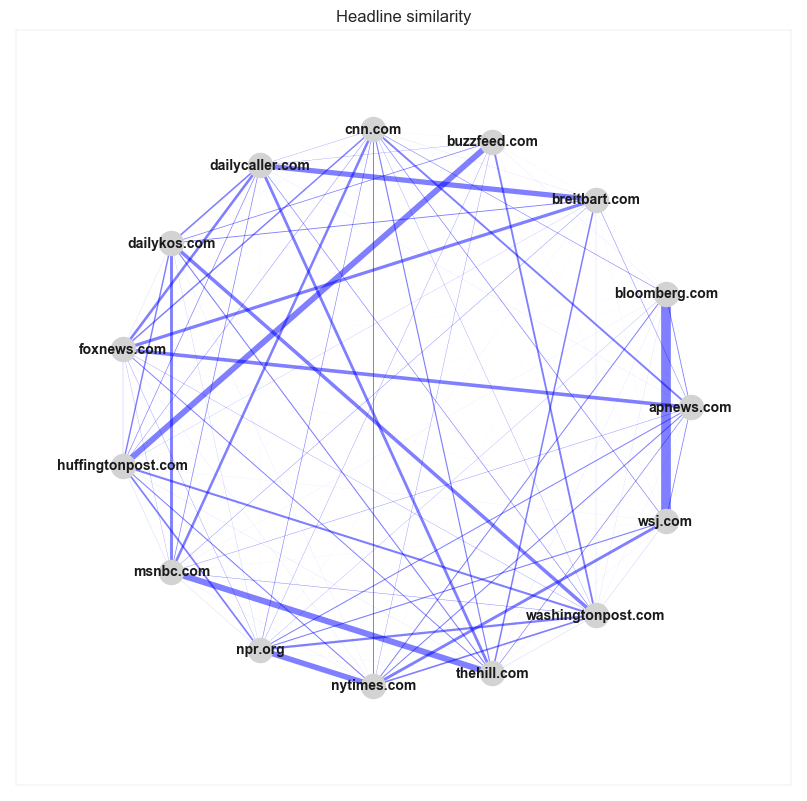
\includegraphics[height=0.5\textheight]{figures/hl-graph-radial-all-metrics.png}
\end{figure}

This question of the \textit{distinguishability} or \textit{separability} of headlines touches on question that sits at the core of a number of recent studies that have explored processes of fragmentation and polarization in the media ecosystem. Building generally on the widely-popularized notions of "filter bubbles" and "echo chamgers" developed Pariser\cite{pariser2011filter} and Sunstein,\cite{sunstein2003republic} a rich line of work has started to document the degree to which new patterns of news production and consumption have pushed audiences into more isolated spaces where they're less likely to encounter counter-attitudinal views. Flaxman et al. analyzed a large dataset of web browsing histories (volunteered by users of a browser extension) and explored the degree to which different patterns of content discovery push readers towards more or less ideologically polarized content, arriving at interestingly mixed results -- social media and search engines expose users to more polarized content, but also expose them to a wider range of views.\cite{flaxman2016filter} Meraz studied the structure of hyperlinks among a set of political blogs during the 2012 presidental election, finding that left-leaning sources were more densely connected than right-leaning sources.\cite{meraz2015quantifying} And, most recently, Benkler et al. explored the outsized influence of right-leaning blogs -- particularly Breitbart -- on media coverage during the 2016 presidental election, building on a map of the media ecosystem derived from correlations in sharing patterns on Twitter and Facebook.\cite{benkler2017study} (The same technique used to model audience-level similarity later in this study).

In many cases, these projects have started by mapping the media ecosystem in terms of these relationships among outlets at the level of \textit{audience} composition -- overlap at the level of readers, viewers, listeners. Once this audience-level snapshot is in hand, though, it then somehow needs to be mapped against salient difference in \textit{content}, the actual substance of the coverage, which plays at least as much of a role in processes of fragmentation and polarization as does the question of audience distance -- if all outlets produced identical content, then audience fragmentation wouldn't matter. Concerns about filter bubbles and echo chambers are fundamentally about an interaction between the "audience graph" and "content graph" -- specifically, when they become both highly fragmented and also highly aligned, when isolated audiences are being exposed to isolated content.

How to operationalize these differences at the level of conent? In a number of cases, content-level similarities have been derived directly from audience composition -- for example, the percentage of an outlet's audience that follows Trump or Clinton on Twitter, voted for a Republican candidate in last election, etc. Where, of course, the assumption is that differences at the level of content are strongly correlated with differences in audience; the content of an outlet is defined in terms of who reads it. Recently, some studies has gone beyond this, most notably in the context of the Media Cloud project at the Center for Civic Media at the MIT Media Lab. Chuang et al. trained topic models on a corpus of 430,000 news articles, giving a high-level view of which outlets focus on which issues -- Forbes on business news, CNET on technology, The Washington Post on President Obama.\cite{chuang2014large} Most recently, Benkler et al., in describing the impact of Breitbart on the 2016 election, conduct a sentence-level analysis of the amount of coverage dedicated to different scandals associated with Clinton and Trump, and measure the degree to which different outlets focused on issues related to immigration.

Generally, though, less is known, about content graph than audience graph. Or, at least -- our knowledge about content graph is less precise. One reason for this, perhaps, is that measuring "textual distance" -- the level of similarity or dissimilarity between documents -- is fundamentally more complex and open-ended than measuring similarity at the level of audience, where outlets are often connected in unambiguous ways that can simply be counted -- the number of shared followers, the number of times the same user tweets articles to two outlets, etc. Whereas with text, as Underwood notes, the question how to meaningfully score the similarity between two documents is a strand that unravels into a large and difficult set of questions. \footnote{It could be argued, in fact, that a sizable portion of nascent field of "cultural analytics", an offshoot of the digital humanities focused on text analysis, is concerned with some formulation of this exact question.}

If we approach this head-on, though -- what could we learn from a very precise representation of the content graph? Beyond just describing differences in an exploratory, unsupervised setting, can we quantify them with a level of rigor and systematicity that would match the precision with with we can model audience level similarities among outlets? How to \textit{measure} them in a way that would make it possible to put them back into conversation with other quantitative views of the media ecosystem?

This is fundamentally the question that this thesis takes up. My conjecture is that there are a number of intersting (but difficult) questions that become tractable when we're able to precisely quantify these content-level similarities. First, if we can say, for example that outlets A and B are 1.0 apart, and B and C are, say, 1.6 apart, then this makes it possible to directly compare the content graph to the underlying audience graph in a very fine-grained, high-resolution way. Which, in turn, opens the door to empirical study of the fundamental assumptions around notions of media polarization and fragmentation. Instead of simply assuming that content and audience move in lockstep -- how true is this actually? And, maybe most interesting -- when, if ever, is this not true? Are there cases of \textit{misalignment}, where, for example, two outlets produce similar content, but have highly disjoint audiences that divide along ideological or cultural lines -- content that serves as a bridge across some axis of social difference? If these sites of  misalignment do exist -- what do they look like, and what might be learned from them?

Second -- by precisely quantifying the (dis)similarity among outlets, it becomes possible to study the content landscape of news as a historically evolving system. Can hypothesize a kind of plate tectonics among media brands, slow processes of drift, change, reorganization, evolution. If we can assign a precise score to the degree to which a pair of outlets is similar or different, then we can also track this measurement over time, and identify the the degree to which the content landscapen is rearranging itself. When tracked over a span of months or years, how stable are the relationships among major media brands? Are some outlets moving faster than others? Where are they moving? Where are things headed?

In other words -- by \textit{quantifying} similarities at the level of content in precise ways, we can then \textit{contextualize} those differences in meaningful and actionable ways.

This thesis, then, explores three questions: (1) How different, precisely, is the content produced by different media organizations? (2) How do (or don't) these similarities at the level of content align with similarities at the level of audience? Does similarly of content correlate with similarity of audience? Where, if ever, does this break down? What could we learn from these sites of mismatch, where audiences are being exposed to issues, styles, viewpoints that they otherwise would be unlikely to encounter? And (3) separate from the regular churn of news coverage from day to day -- how have outlets changed over time in terms of the type of coverage they produce? What has changed, what's changing?

In summary, we find:

\begin{enumerate}

\item Modeled as a text classification task, headlines from 15 major US media sources highly differentiable, even after an aggressive cleaning process that strips out any kind of "paratext" in the headline that directly or indirectly reveals the source. (For example, "... -- CNN Video" or "AP Breaking News: ...") The strongest model is a bidirectional LSTM, which gets to 41\% accuracy in a 15-label model, where random would be 7\%. Though, standard non-neural baselines also perform very well -- SVM and logistic regression models over ngram count features are competitive at 36-38\% accuracy (and beat the weaker neural models), suggesting that a majority of the differentiability among outlets comes from which words and phrases are being used -- roughly, what might be thought of as "topic" or "content" -- and less from the composition or sequencing of words, which can be modeled with more power by the recurrent models.

\item Pulling sentence embeddings out of the top layer of the LSTM, we can explore the structure of the linguistic space in terms of the high-dimensional representations learned by the model, both in terms of the relationships among different outlets are the internal structure of the headlines within the outlets themselves. This reveals significant differences in what might be thought of as the "shape" of different outlets in the high-dimensional space. Specifically, we focus on what we call the "diameter" of the embedding family for each outlet -- the average cosine distance between randomly sampled pairs of headlines -- which, we argue, roughly captures the degree to which outlets are narrowly focused (low diameter) or more broad and varied (high diameter). Second, we also explore the clustering structure of headlines within outlets, the degree to which content from an outlet can be cleanly decomposed into a set of categories, verticals, or "desks." On both metrics, we find significant variation, with BuzzFeed, Bloomberg, and Daily Kos registering the lowest "diameters" and smallest cluster counts (most focused), and CNN, The Washington Post, and Fox showing the highest diameters / largest cluster counts (most broad, varied, diverse).

\item Aggregating over the full set of individual articles in each outlet, we can use the classifiers to model a complete "content graph" among the 15 organizations, a fully-connected graph of pairwise similarity scores, which are extracted from the behavior of the classifiers in a collection of different ways -- pairwise accuracy scores, probability mass correlations in multi-label models, and confusion counts. With this content graph in hand, we then compare to the underlying "audience graph," derived from correlations in the users who tweet links from each pair of outlets. From these two graphs, for each outlet we can construct two normalized rankings of similarity with all other outlets, one based on headline similarity, and the other based on audience similarity. We then explore the correlation of these two rankings on a per-outlet level -- that is, the degree to which an outlets edge weights in the "content graph" are similar to its edge weights in the "audience graph."

In general, we find that these two sets of weights tend to be positively correlated, often highly so -- in general, outlet A "sounds like" outlet B, it also has a high level of audience overlap. But, there is a wide range in the strength of this correlation, and there are some strong exceptions -- namely The Associated Press and The Hill, both of which show a significant level of misalignment between their content and audience graphs, with correlations of roughly 0. For AP, this is driven by Fox, which both syndicates a sizable number of articles from AP and also produces in-house content that closely resembles AP. But, by and large, this AP-style content is dramatically different from the rest of the coverage produced by Fox, and represents arguably the most significant content-audience mismatch in the dataset. After the AP (which is anomalous in that it's a wire service, and AP content gets literally "duplicated" by other outlets), The Hill seems to be the closest thing to a naturally "bridging" or "bipartisan" outlet -- it has high audience overlap with left-leaning outlets, but high headline similarity with the right-leaning Daily Caller and Breitbart; but also with the left-leaning MSNBC.

\item We then explore the evolution of these relationships over historical time -- instead of treating the corpora as a monolithic bundle of data, the 2-year data window is broken into 100 temporal bins, and a 10-bin rolling window is moved across this space, producing 91 10-bin windows. In each of these windows, we train fully independent A-versus-B models on each unique pair of outlets, and then track changes in these accuracies over time. This reveals significant changes in the structure of the content graph in the last two years. First, The Huffington Post and BuzzFeed have moved away from each other, due to mirror-image changes -- HuffPo has moved away from "clickbait" content (advice colums, diet recommendations) and towards more narrowly-focused political reporting, similar to The Hill, DailyKos, and CNN; whereas BuzzFeed doubled down on clickbait content (specifically, a certain type of "quiz" article), pushing down the proportion of content from BuzzFeed that consists of serious political and investigative reporting. Second, a cohort of politically-focused outlets have become more similar -- The Hill, The Daily Kos, CNN, AP, NYT, WaPo, NPR -- suggesting a tendency towards convergence in political coverage since a high-water mark of differentiability in the spring of 2017, in the first months of the Trump administration. Last -- Fox has consistently moved away from almost all other outlets, including other right-leaning outlets like Breitbart and The Daily Caller; it has become much more highly differentiated \textit{individually}, compared to everything else. By examining headlines that typify the overall movement of Fox in the high-dimensional linguistic space modeled by the neural classifier, it appears that this shift is driven by a move in the direction of a highly sensationalized, tabloid style of headline, many of which involve violent crime and socially-charged political issues.

% TODO: update
\item Finally, we also unroll the audience graph over these temporal windows, and explore the degree to which changes in the content graph correlate with changes in the audience graph -- as two outlets produce increasingly similar content, do their audiences also become more overlapping? Overall, we find a positive correlation here, though the relationships for individual pairs of outlets are interestingly varied. In some cases, the content / audience similarities for a pair of outlets move in almost perfect lockstep, sometimes even at the scale of months or weeks -- for example, AP / Huffington Post, Huffington Post / MSNBC, Bloomberg / Fox. But, in other cases, content and audience appear to have an almost perfectly *negative* correlation. For instance, over the last two years, Breitbart and Fox have become very consistently less similar in terms of content, but consistently *more* similar in terms of audience. Or, Breitbart and CNN have had a fluctuating level of similarity at the level of content, and an almost perfectly inverse fluctuation of audience similarity -- when content is similar, audience is dissimilar, and vice versa. These differences suggest that the underlying causal relationships between changes in content and changes in audience are complex, and likely different for different combinations of media organizations.

\end{enumerate}

\section{Headlines on Twitter}

To explore this interaction between content and audience, we need what might be thought of as a "networked" corpus -- a collection of individual pieces of content that can be linked to specific patterns of audience engagement.

To get a snapshot of the content produced by different news outlets, we could just scrape their websites directly. But, with this in hand, it would difficult to then consisently map this text data back to fine-grained patterns of audience behavior -- just from the raw pages, we have no way to know who read them, when, paired with what, etc. And, even if we had access to some approximation of this from internal data collected by the news organization, it would then be difficult to link this across multiple outlets and get a holistic view of how the same readers engage with multiple sources.

This is where data from centralized services becomes very valuable -- from platforms like Twitter or Reddit, we can get information about uniquely identified users interacting with content from a range of sources in the context of a (relatively) controlled setting. For example, Flaxman et al. used browser history volunteered by users of the Bing Toolbar, an extension for Internet Explorer. Here, we follow Benkler et al. in using \textit{links to news articles shared on Twitter} as the fundamental unit of data.\footnote{Of course, we have no interest here in characterizing the behavior of specific users -- we're interested in behavior at the \textit{scale} of the individual user, but only in the aggregate, spread across tens of millions of accounts. This study never reports any text data or sharing activity that could be linked back to individual people.}

For example, working with the Decahose, a 10\% sample of Twitter -- if someone posts a tweet with a link to a New York Times article, Twitter detects the link and provides structured information about it in the JSON payload that appears in the Decahose:

\begin{lstlisting}
"urls": [
    {
       "url": "https://t.co/MOZgWRzhRK",
       "expanded_url": "https://www.nytimes.com/2017/09/27/us/politics/navy-orders-safety-operational-standards.html",
       "display_url": "nytimes.com/2017/09/27/us/…",
       "indices": [66, 89]
    }
 ],
\end{lstlisting}

We can then parse the raw URL string and extract the registered domain -- here, \texttt{nytimes.com} -- which makes it possible to associated URLs with different media organizations.

Critically, though, this study also makes use of the "Enhanced URLs" data available through Gnip, the vendor that distributes data from Twitter. The "Enhanced URLs" metadata provides two pieces of information that are essential to this study -- first, the "expanded" URL, which is formed by following redirects from the raw URL that appears on Twitter. This valuable here because a fairly large number of links on Twitter are passed through URL shorteners like \texttt{bit.ly}, meaning that they have to be "unrolled" in order to identify out the real domain -- for example, \texttt{nytimes.com} instead of \texttt{bit.ly}. In theory, we could do this ourselves; but, especially when working with data that's more than a few weeks old, this can be difficult. Many of these services automatically expire the links after a certain amount of time, meaning that, for example, if we tried to expand a link from spring of 2017, it would likely fail.

Second, and most important, "Enhanced URLs" also provides scraped copies of the \href{http://ogp.me/}{Open Graph} \texttt{title} and \texttt{description} tags of the page that the link points to. At a product level, Twitter uses the title and description in the preview boxes for the article that get displayed below the tweet that contains the link.

\begin{lstlisting}
"gnip": {
  "urls": [
     {
        "url": "https://t.co/MOZgWRzhRK",
        "expanded_url": "https://www.nytimes.com/2017/09/27/us/politics/navy-orders-safety-operational-standards.html",
        "expanded_status": 200,
        "expanded_url_title": "Navy Returns to Compasses and Pencils to Help Avoid Collisions at Sea",
        "expanded_url_description": "A top officer issued new orders to sailors worldwide as the Navy scrambled to make priorities of safety and maintenance after two deadly collisions in recent months."
     }
  ]
},
\end{lstlisting}

This, in a sense, gives us precisely what we need -- a representation of content (headlines), directly linked to a representation of audience (Twitter users, tweets). What are the implications of using Twitter, though -- or, for that matter, headlines?

With Twitter -- the downside, of course, is that Twitter, in well-documented ways, isn't representative of the full media ecosystem; it's one specific social network, and in many ways an idiosyncratic one. But, the advantage is that we can explore these questions with a level of scale and, perhaps even more important, consistency that would otherwise be impossible. Twitter prevents us from making "wide" claims about the media ecosystem -- we can at most make "platform-studies" claims about what happens on Twitter. But, with this loss of generality, we also gain the ability to explore these questions with a level of depth and specificity that would otherwise likely be impossible. Twitter is just one part of the media ecosystem; but we can get a very high-resolution view of that one part.

As for using headlines -- the downside, clearly, is that we don't get a view of the full content in the underlying articles. And, the relationship between headlines and the corresponding article text is somewhat unclear, meaning that we can't use the headlines as a proxy for the full content profile of an outlet. But, at the same time -- headlines themselves are incredibly interesting textual objects, an elusive mix of summary, advertisement, quotation, metonymy,\cite{shie2011metaphors} provocation. And, beyond the linguistic and (and even para-literary) interest of headlines, there are a number of more intellectually pragmatic advantages to focusing on headlines in this context.

First, to the extent that we're interested in studying the interplay between content and audience, headlines are generally the content with highest level of "colocation" with audience activity on Twitter -- when someone tweets a link, the headline is usually literally displayed with the tweet. (Though this can vary, depending on the specific product context, the client being used.) There's a kind of "physical" proximity between headlines and the corresponding reader behavior on Twitter that's methodologically attractive -- when a user interacts with a news article on Twitter, it's often in response to the headline.

Second, far from being a kind of inconsequential paratext that get tacked on top of the "real" content in the articles themselves, there's a (perhaps distressing) way in which headlines just \textit{are} the news, in a constituitive sense. According to a 2014 survey from the American Press Institute, just ~41\% of Americans said that they had "watched, read, or heard any in-depth news stories, \textit{beyond the headlines}, in the last week" (emphasis added).\cite{api2014rational} Headlines represent extraordinarily high-leverage langauge. If we imagine placing different types of textual objects on a continuum that represents the level of social, political, economic "stopping power" that they command -- then headlines, on a per-word basis, would sit very near (if not at) the top of this list. If we're interested in the sites at which language \textit{acts} on the world in manifest ways -- headlines are hard to beat.

We also have the advantage of building on a rich lines of work in media studies, sociology, psychology, and (computational) linguistics that have studied headlines from several perspectives. In the tradition of content analysis, a number of projects have examined the depiction of specific issues in newspaper headlines -- portrayals of Muslims in British newspapers,\cite{bleich2015media} accounts of Boko Haram in Nigerian newspapers,\cite{abba2015speech} post-traumatic stress in the New York Times,\cite{purtle2016calculating} coverage of robotic surgery,\cite{ficko2017high} the impact of headlines about generics research on beliefs about genetic determinism,\cite{condit2001exploratory} and the stylistic properties of headlines in science journalism.\cite{molek2017stylistic}

At a more theoretical register in the linguistics literature, Dor\cite{dor2003newspaper} describes headlines in the context of linguistic notion of "relevance optimization" -- headlines try to maximize "contextual effects" for a reader, while also being short and easy to process. In a sense, this threorization of headlines, represents an ideal framing for the question here about the iterplay between content and audience -- Dor essentially describes them as highly condensed sites of negotiation between content and audience, textual objects that try to bridge the gap, as efficiently as possible, between the substance of the article and the assumptions and expectations of the (assumed) reader.

Meanwhile, in the natural languge processing literature, there are two active lines of work that have focused on headlines. First, a series of studies that treat headlines as evidence about the future, in different ways -- in quantative finance, a number of studies have explored correlations between news headlines and price movements in different kinds of investment vehicles.\cite{chan2003stock}\cite{jotaki2018analyzing}\cite{meyer2017fine}\cite{ghosal2017iitp} And, other work has focused on predicting the the "performance" of headlines themselves in the content marketplace of the web -- diffusion on social networks, click-through rates, etc.\cite{kim2016compete}\cite{gabielkov2016social}\cite{piotrkowicz2017headlines}\cite{trilling2017newsworthiness}\cite{reis2015breaking} Meanwhile, alongside this -- another line of work has focused on what might be thought of as "pathalogical" headlines. For example, a number of studies have examined "clickbait"\cite{blom2015click} or "sensational"\cite{molek2013towards} headlines and explored the degree to which they can be automatically flagged by classifiers;\cite{chen2015misleading}\cite{chakraborty2016stop} or identifying cases where the headline doesn't match the underlying article content.\cite{chesney2017incongruent}\cite{ecker2014effects}\cite{wei2017learning}\cite{bourgonje2017clickbait}

Like these studies, we approach headlines from a standpoint of prediction -- in our case, predicting the \textit{origin} of the headline. But, instead of trying to solve an  engineering problem, we use the supervised learning problem as a descriptive and interpretive tool -- a way to measure the similarities between headlines, and a way to induce representations of headlines that make it possible to "read" the news ecosystem at a scale that would otherwise be impossible.

\section{5.65 billion links}

So -- tweets with links, and links that point to headlines. Before diving into the headlines themselves -- what does this data look like in its native environment on Twitter? In this study, we work with an archive of the Decahose that was collected by Cortico, a non-profit organization affiliated with the Laboratory for Social Machines. Specifically, we focus on a 625-day window of data running from January 1, 2017 through September 17, 2018. Over that period, the Decahose emitted 21,219,935,342 total tweets. Of these, 5,243,960,217 (24.7\%) include at least one link.

Where do these links point? As an first step, we can parse the raw URL strings into component parts (protocol, subdomain, registered domain, path, etc.) and then count the total number of links to each registered domain. These are the 100 most frequently-occurring domains, before any filtering is applied:

\begin{displayquote}
\scriptsize \raggedright twitter.com, youtube.com, du3a.org, facebook.com, instagram.com, d3waapp.org, google.com, curiouscat.me, tistory.com, ghared.com, naver.com, zad-muslim.com, showroom-live.com, twittascope.com, ebay.com, fllwrs.com, vine.co, amazon.com, 7asnat.com, apple.com, channel.or.jp, blogspot.com, twitcom.com.br, soundcloud.com, nytimes.com, yahoo.co.jp, cnn.com, nicovideo.jp, pscp.tv, swarmapp.com, spotify.com, ameblo.jp, 7asnh.com, tumblr.com, line.me, wordpress.com, daum.net, washingtonpost.com, twitch.tv, twitcasting.tv, insurancepremium-wd.com, seesaa.net, shindanmaker.com, amazon.co.jp, dmm.co.jp, thehill.com, theguardian.com, etsy.com, imgur.com, bbc.co.uk, paper.li, foxnews.com, fc2.com, rakuten.co.jp, careerarc.com, gleam.io, reddit.com, ask.fm, monster-strike.com, quran.to, lawson.co.jp, reuters.com, staticflickr.com, globo.com, peing.net, billboard.com, soompi.com, grandesmedios.com, medium.com, hotpepper.jp, crowdfireapp.com, nhk.or.jp, twimg.com, vlive.tv, breitbart.com, alathkar.org, tuitutil.net, sinaimg.cn, huffingtonpost.com, go.com, buzzfeed.com, dailymail.co.uk, elpais.com, livedoor.com, change.org, utabami.com, livedoor.jp, vonvon.me, pixiv.net, rt.com, bbc.com, politico.com, daumcdn.net, yahoo.com, independent.co.uk, asahi.com, linkedin.com, naver.jp, nbcnews.com
\end{displayquote}

A majority of these, of course, don't represent "news" sources in a meaningful sense. Though, this isn't always clear-cut -- for example, links to Facebook might often point to content from news organizations that has been shared on Facebook. But, bracketing this, and just operating at the level of individual media brands -- if we take the 2,000 domains with overall largest link counts and then manually filter this list, we can pull out a long list of 87 major media organizations. Of course, "major" is somewhat subjective; here, we took all outlets that meet a minimum standard of name recognition and produce either "general-interest" news or political reporting / commentary; but not specialized outlets that focus on topics other than politics -- ESPN, TechCrunch, Rolling Stone, etc. Here are these 87, ordered here by the total number of links:

\begin{displayquote}
\scriptsize \raggedright nytimes.com, cnn.com, washingtonpost.com, thehill.com, theguardian.com, foxnews.com, bbc.co.uk, reuters.com, breitbart.com, huffingtonpost.com, buzzfeed.com, politico.com, rt.com, independent.co.uk, yahoo.com, nbcnews.com, bloomberg.com, forbes.com, wsj.com, thegatewaypundit.com, businessinsider.com, usatoday.com, cbsnews.com, apnews.com, dailycaller.com, rawstory.com, vice.com, npr.org, truepundit.com, thedailybeast.com, time.com, cnbc.com, telegraph.co.uk, newsweek.com, nypost.com, sputniknews.com, nydailynews.com, washingtonexaminer.com, cbc.ca, vox.com, thinkprogress.org, theatlantic.com, newyorker.com, msn.com, ft.com, slate.com, theroot.com, variety.com, inc.com, dailykos.com, judicialwatch.org, msnbc.com, motherjones.com, aljazeera.com, economist.com, washingtontimes.com, dailywire.com, infowars.com, theintercept.com, axios.com, theonion.com, politicususa.com, thetimes.co.uk, nymag.com, salon.com, qz.com, nationalreview.com, palmerreport.com, townhall.com, thefederalist.com, hbr.org, hannity.com, talkingpointsmemo.com, fortune.com, thenation.com, propublica.org, foreignpolicy.com, theblaze.com, pbs.org, foxbusiness.com, theconversation.com, conservativereview.com, fivethirtyeight.com, crooksandliars.com, jezebel.com, newrepublic.com, realclearpolitics.com
\end{displayquote}

\begin{figure}[H]
  \centering
  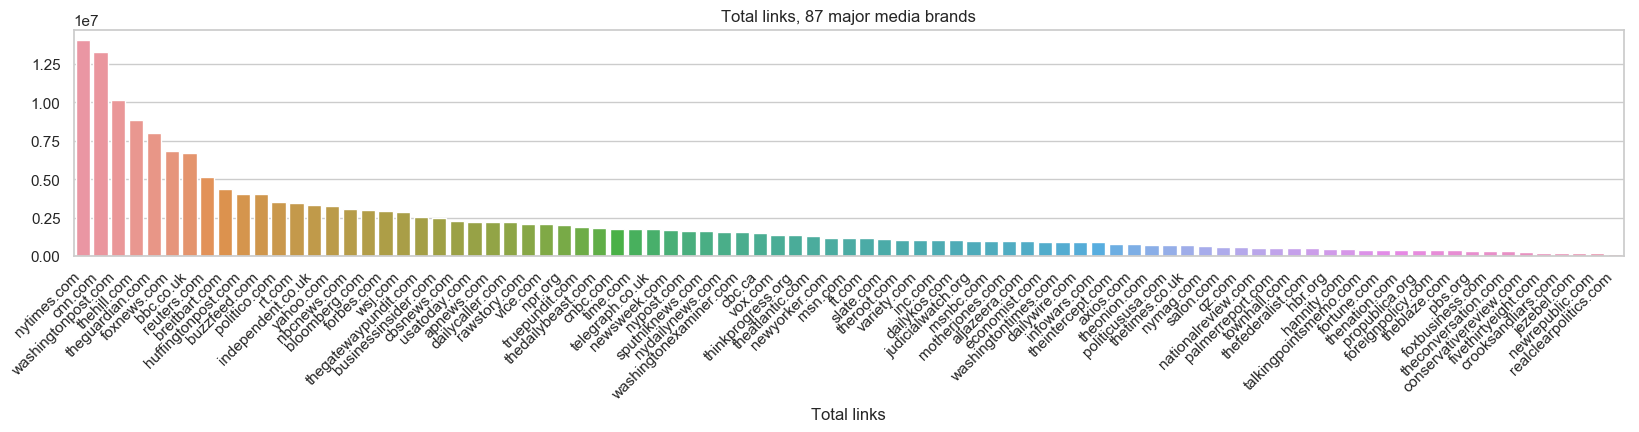
\includegraphics[width=\textwidth]{figures/t87-link-counts.png}
\end{figure}

Which, collectively, account for 73,198,274 million individual links in the data. The total number of links, though, is very different from the number of \textit{unique articles} -- a single article might produce tens or hundreds of thousands of individual tweets linking to the same piece of content, each of which are counted separately here. One simple way to roll up the individual occurrences of the domains by article is just to group on the exact text of the URL. But, this is somewhat brittle, since it's not uncommon for links to get passed around with superfluous GET parameters added onto them (eg, trackers that flag the source of a click). This can cause the same "base" URL to appear in many different configurations, if just treated as a raw string, all of which in fact point to the same article.

Instead, we group links into articles by combining three pieces of information -- the registered domain, the "path" component of the URL, and the cleaned tokens in the Open Graph title, as provided by Gnip. (This cleaning process is somewhat intricate, detailed below.) The URL path is taken into consideration since there are times when the same outlet will produce multiple articles with identical titles. For example, if The New York Times produces an article every week called "Your Monday morning roundup" -- by including the URL path as part of the grouping key, we can correctly identify these as legitimately separate pieces of content.

Grouping links on these three pieces of information, we can count the number of unique articles (and, by extension, headlines) associated with each domain. Which, in this context, is the more salient number, since the headline is the basic unit of analysis. The largest outlets have produced many hundreds of thousands of individual articles in the last two years, though the volume falls off fairly quickly outside the top ~20:

\begin{figure}[H]
  \centering
  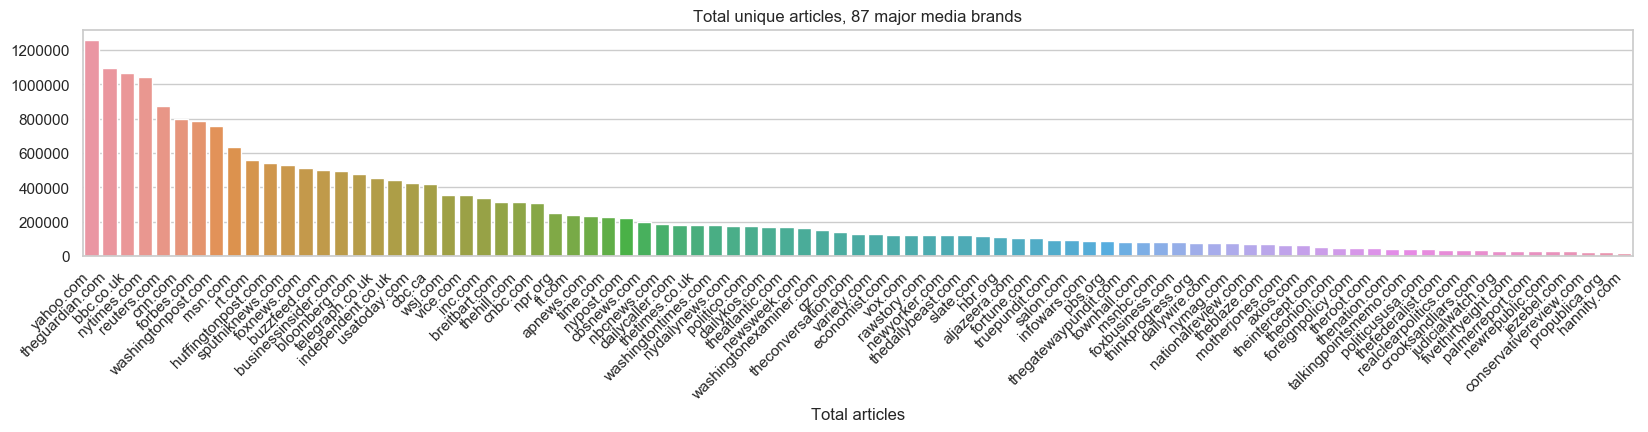
\includegraphics[width=\textwidth]{figures/t87-article-counts.png}
\end{figure}

Beyond these rolled-up link and article counts, we can also easily get a high-level sense of how the footprint of different outlets on Twitter has evolved over the 2-year data window. Using the \texttt{postedTime} timestamps on each tweet, we can group links from an outlet by day, for instance, and look at the historical volume trend. For The New York Times:

\begin{figure}[H]
  \centering
  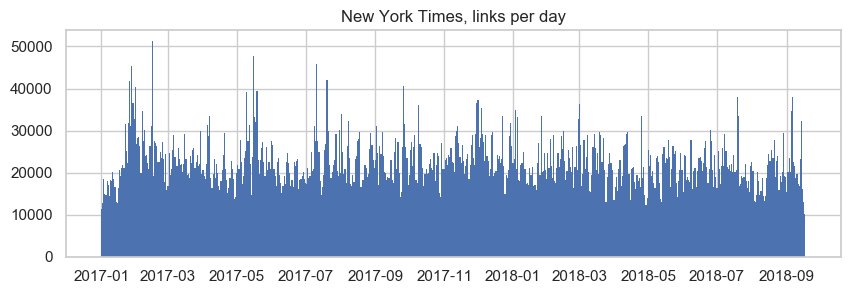
\includegraphics[width=\textwidth]{figures/nyt-links-per-day.png}
\end{figure}

Or, rollup up links by article, the total number of unique NYT articles that appeared by day:

\begin{figure}[H]
  \centering
  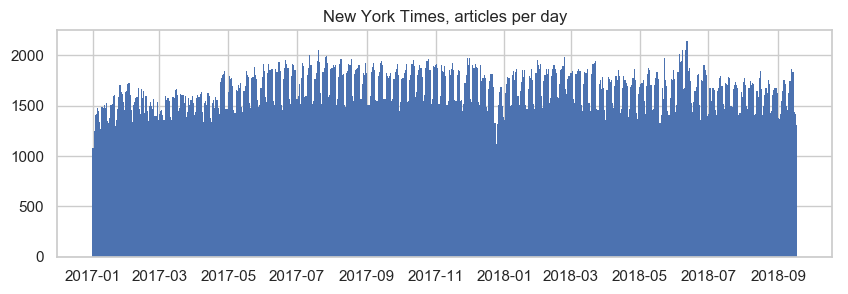
\includegraphics[width=\textwidth]{figures/nyt-articles-per-day.png}
\end{figure}

Finally, digging deeper into the metadata provided by Twitter -- for each tweet, we also have information about the user account that posted the tweet, including the follower count of the user at the time the tweet was posted. This is very useful information, since follower counts vary significantly -- a link posted from an account with 1M followers will have vastly more reach than a link posted from an account with 100 followers. In a crude sense, we can use the follower count of the user account as a proxy for "impressions," the total number of times that the tweet was seen by individual twitter users. (Of course, this isn't literally true -- when a user posts a tweet, the percentage of her followers who actually see it is probably fairly low, since many of them won't be logged on, etc. But, if we assume that this percentage is roughly similar across the platform, the follower count can give a (relative) signal of the real-world "reach" of the tweet.)

Taking the total impressions produced by all tweets with links to The New York Times, and grouping by day:

\begin{figure}[H]
  \centering
  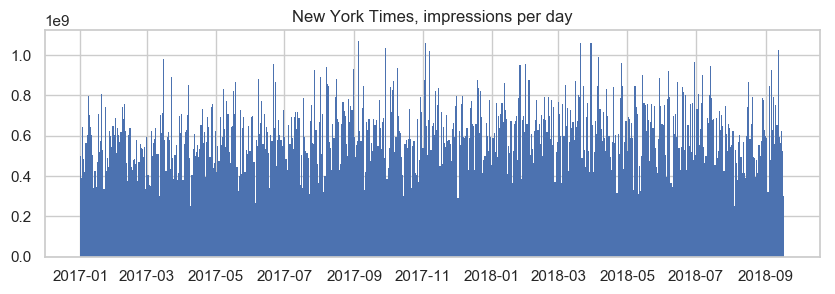
\includegraphics[width=\textwidth]{figures/nyt-imp-per-day.png}
\end{figure}

Some of which, interestingly, show very significant changes over the 2-year data window. Modeling this as a linear trend, here are the 10 domains with the most significant decreases, in terms of links, articles, and impressions:

\begin{figure}[H]
  \centering
  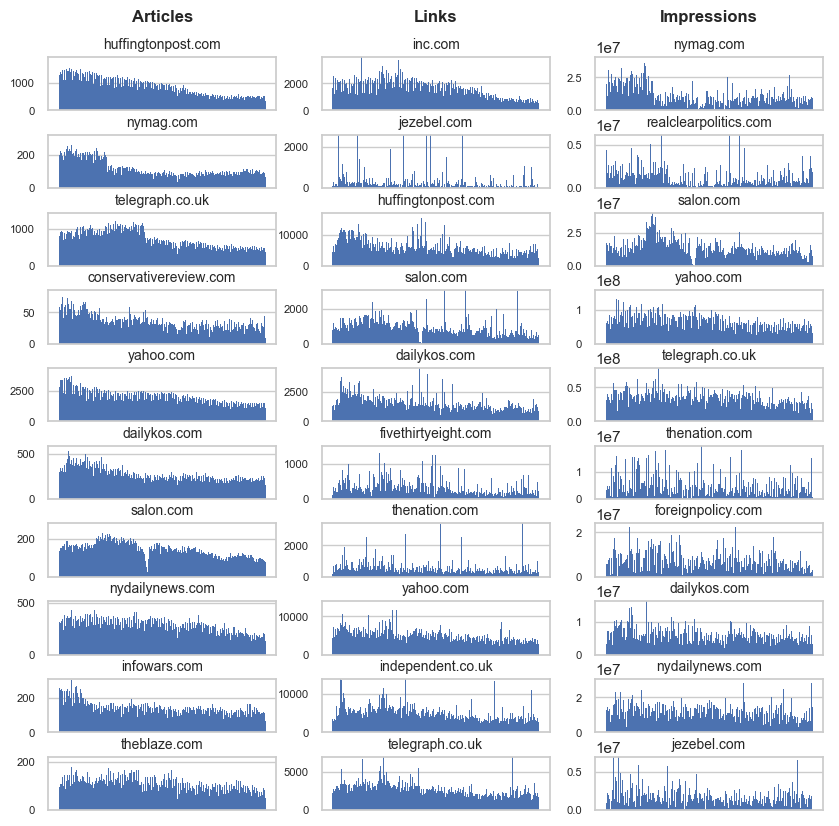
\includegraphics[height=0.6\textheight]{figures/vol-dec.png}
\end{figure}

So, the number of unique articles from Huffington Post, on a per-day basis, has fallen by more than 50\%. In the other direction, domains with the strongest increases in volume:

\begin{figure}[H]
  \centering
  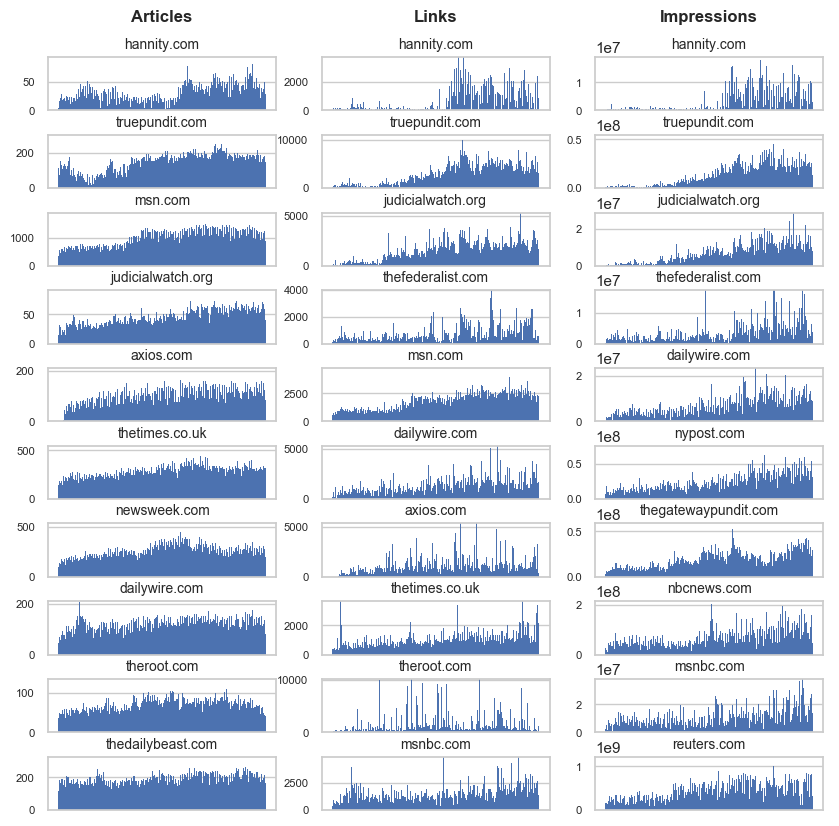
\includegraphics[height=0.6\textheight]{figures/vol-inc.png}
\end{figure}

Which has a striking partisan tilt: all of the four domains at the top of the three lists -- \texttt{hannity.com}, \texttt{truepundit.com}, \texttt{judicialwatch.com}, \texttt{thefederalist.com} -- represent (far) right-leaning political perspectives.

Of course, we don't really care about the "performance" of the headlines per-se -- our focus here is on the structure of the linguistic relationships among outlets. But, these overall volume trends have important methodological implications, especially for the historical questions that emerge in the second half of the project. Namely, if we're interested in exploring changes in relative similarity between outlets over time, it's clear that we need to explicitly standardize for these changes in volume, to prevent them from getting artificially proxied by other measurements. For example, if we use classification accuracy as a measurement for similarity, a model trained on HuffPo data from 2018 will almost certainly be lower-performing than a model trained on 2017 data, just because the 2018 model will see far less evidence -- even though the actual coverage might not have changed in any meaningful way, just the quantity of coverage.

But, there's only so much we can learn by just counting links, articles, users, impressions; what we really want is a meaningful understanding of the relationships among the outlets -- how similar are the headlines? How similar are the audiences? Where they differ -- how, exactly?

\section{Modeling textual distance with classification}

From the Decahose, then, we can extract a set of unique article headlines that have appeared in the Decahose over a ~2-year period from a set of 87 major US media brands, aggregated from a complete set of 73 million individual links posted on Twitter.

Given just the raw headline strings pulled from the \texttt{og:title} tags -- how can we reason about the relative similarities and differences between the headlines from different outlets? For example, say we have 300k unique headlines from NYT, 200k from CNN, 50k from Daily Caller -- how similar or different, in a precise sense, is each pair of outlets? Or, considered as a group -- what does the overall matrix of similarities look like? What clusters with what? Which topics, styles, entities, textual features drive these similarities and differences? If we think of the full set of 1.1 million unique headlines as representing a kind of linguistically-instantiated landscape -- what's the shape of this space, what's the linguistic "topography" of headlines on Twitter?

There are various we could model this. Here, though, we follow Underwood et al.\cite{underwood2018transformation}\cite{underwood2018historical} in framing the question as a \textit{predictive} task -- we explore the structure of the data by studying the degree to which we can train models to learn accurate mappings between headlines and outlets. That is -- if we have headlines from outlets A and B, we can train a lexical classifier to predict whether a given headline was produced by A or B? If the model achieves a high accuracy on test data -- if it is able to learn significant structure across the two classes and perform well on unseen data -- then this can be interpreted as a signal that the two sets of headlines are highly "separable" or "distinctive," given the representational capability of the model. And, conversely, if the model achieves poor accuracy -- if it has a hard time telling the difference between A and B -- then we can interpret this as a signal that the headlines are relatively similar. At the extreme edges -- if the model achieves 100\% accuracy, then we can interpret this as being the maximum possible "distance" between outlets -- they are completely differentiable. And, if the model achieves 50\% accuracy on a balanced sample, no better than random, then we can interpret this as the smallest possible distance between outlets, a distance of 0 -- they are effectively indistinguishable.

(To the model, at least. With interpretive projects like this, where we're trying to model "meaning" in text, in some way, we always have to keep in mind that there's a mismatch between what a machine learning model "sees" in a piece of text and what a real person would see. Sometimes the model will fail to pick up on something that would be obvious to a real reader; other times the model will latch onto details that might seem insignificant to us. But, if we're willing to accept this quotient of interpretive slippage -- computation makes it possible to "read" these kinds of large corpora with a level of scale and comprehensiveness that would otherwise be impossible.)

There are various other ways we could go about this, but, there two big advantages to formulating the question as a predictive task. First, it provides a number of natural ways to extract a very simple and interpretable \textit{metric} that captures relative differences in similarity. For example, when predicting whether a headline comes from AP News or BuzzFeed, the model might get to 85\% accuracy; but just 60\% accuracy when comparing Bloomberg and WSJ.

Second, in the context of modern neural architectures, the classification task provides a natural training objective for learning high-quality, corpus-specific \textit{representations} of the headlines. If we train custom deep learning models to predict an outlet given a headline, it's easy to then extract the underlying sentence embeddings that are induced by the model -- high dimensional vectors that represent the "meaning" of the headline, as operationalized by the classifier.

These embeddings give a remarkable interpretive power -- they can be treated, essentially, as a set of coordinates that position each headline in a high dimensional space, and we can then study the "shape" of the linguistic landscape defined the headlines, both within individual outlets and among them. And, at a more pragmatic level -- the embeddings also make it possible to systematically find individual examples that are typical, in various ways, of salient changes that are observed at the level of corpus averages. For example -- if we identify some kind of smooth, gradual change in the similarity between two outlets over time, we can query the individual headline embeddings in various way to try to find examples that "mark" or "define" the conceptual essence of this movement. The embeddings open the door to a very rich mode of "distant reading," to borrow from Franco Moretti -- the ability to reason in nuanced ways about the meanings contained in very large corpora of text.

\section{Headline differentiability}

We take classification, then, as a modeling paradigm; to understand the headlines, we explore the degree to which we train models that map from headline to outlet. Which, in turn, provides a natural way to precisely measure the similarity between outlets, as well as a training objective that we can use to induce high-quality representations of the headlines.

So -- how differentiable are headlines? Through a lens of statistical inference -- how "learnable" is the relationship between a news organization and the headlines it produces? Ideally, we could explore this question across the full set of 87 media organizations that were culled from the list of the 2,000 most frequently-appearing domains on Twitter. But, because of the fast falloff in the total number of articles associated with each outlet, it's not feasible to analyze all of them. Especially since, in this context, we generally have to downsample everything to the size of the *smallest* outlet -- eg, if we want to compare the accuracy of a model on headlines from outlet A vs outlet B, we have to make sure that the model sees exactly the same amount of "evidence" for each, or otherwise the comparison is unfair. So, if we have ~300,000 headlines from NYT, but only ~3,000 from Judicial Watch, we'd have to downsample NYT by two orders of magnitude -- which seems like a waste, and also starts to feel like something of an apples-to-oranges comparison.

Instead, we pull out a hand-picked set of 15 major outlets, which were selected in an effort to get broad coverage across the largest US media brands and also diversity at the level of political orientation (left-leaning, right-leaning, centrist) and business model (cable news networks, print-and-web newspapers, web-only publications):

\begin{enumerate}
  \item AP News
  \item Bloomberg
  \item Breitbart
  \item BuzzFeed
  \item CNN
  \item The Daily Caller
  \item The Daily Kos
  \item Fox News
  \item The Hill
  \item The Huffington Post
  \item MSNBC
  \item The New York Times
  \item NPR
  \item The Wall Street Journal
  \item The Washington Post
\end{enumerate}

Second, after filtering on these outlets, we also just take articles that received at least 10,000 (potential) impressions, as measured by the sum of the follower counts of the users who posted links to the article. (As mentioned before, this ensures a certain minimum "footprint" for the article, and protects from certain types of sample imbalance that could arise from automated activity on Twitter.) After filtering by domain and applying this minimum impressions threshold, this gives a working corpus of 1,081,790 unique articles, where the largest outlet in terms of volume is The Washington Post, with 122,197 articles, and smallest is MSNBC, with 18,808.

As a first step, we train a series of multiclass models, in which the classifier is presented with headlines drawn from all 15 outlets and trained to predict which outlet produced the headline. To ensure exact comparability across the different architectures, for these benchmarks we freeze off a single downsampled training corpus that is used for all training runs -- 18,808 headlines are sampled from each outlet at the start, and then each model is trained on this frozen sub-corpus of 282,120 headlines.

We compare seven models. First, two non-neural baselines, using standard implementations from the \texttt{sklearn}\cite{scikit-learn} Python package:

\begin{itemize}
\item \textbf{Logistic regression} -- Standard logistic regression under L2 regularization, fit on TFIDF-scaled ngram count features (order 1-3). In the multiclass case, we use the \texttt{sag} solver.

\item \textbf{Linear SVC} -- A standard SVM, fit on the same features.
\end{itemize}

Then, we explore five different neural architectures. All of these models share a common token embedding pipeline, and then implement different line encoders on top of the token embeddings. Tokens are encoded first with a CNN over individual characters, following Kim et al.\cite{kim2016character} -- characters are mapped to 15d embeddings, and then encoded with a CNN with six filter maps of widths 1-6, each with 25 units per character of width and with max-pooling over the feature maps, which produces a 525d embedding for each individual token. This character-level representation is then concatenated with a standard 300d pre-trained GloVe embedding for the token, where one is available, resulting in a composite 825d embedding for each token. then, these token sequences are handed to one of five different line encoders, with increasing levels of complexity:

\begin{itemize}
\item \textbf{CBOW} - Simply the unweighted, dimension-wise mean of all token embeddings in the headline.

\item \textbf{CNN} - A standard CNN for sentence classification as described by Kim.\cite{D14-1181} Though, we use a larger set of filter widths (1-5), each with 500-unit feature maps.

\item \textbf{LSTM} - A standard bidirectional LSTM, using a single 512-unit hidden layer for each direction. The top layers of the forward and backward pass are concatenated together to form a single 1024-unit embedding for the line.

\item \textbf{LSTM + Attention} - Standard attention over the LSTM states, using a separate, two-hidden-layer FFNN to produce scores over the states. As described by Bahdanau et al,\cite{bahdanau2014neural} these weights are interpreted as a probability distribution, which is then use to produce a weighted linear combination across the states, which is then concatenated with the final LSTM output to form a combined 2048-unit encoding.

\item \textbf{LSTM + CNN} - Similar to attention, but instead of using a linear combination over the states, the states are instead treated as higher-order token embeddings and passed through the same convolutional layers used in the standard CNN encoder. Like with the attention network, the output of the CNN is concatenated with the regular LSTM output.
\end{itemize}

All models are all trained under a standard cross-entropy loss, using the Adam optimizer with a learning rate of \texttt{1e-4} and a batch size of 50. The implementation is in Pytorch,\cite{paszke2017automatic} and models are trained on a single NVIDIA V100 GPU, running on a \texttt{p3.2xlarge} node on EC2.

\section{Headline cleaning}

Before comparing across the full set of seven models, though -- how difficult is the task? What kind of performance should we expect? As an initial smoke test -- if we apply a standard tokenization to the raw headline strings that come through the Decahose, and then fit the vanilla logistic regression, we get 50\% accuracy on the full 15-class model:

\begin{lstlisting}
                    precision    recall  f1-score   support

        apnews.com       0.47      0.48      0.47      1909
     bloomberg.com       0.51      0.58      0.54      1942
     breitbart.com       0.77      0.75      0.76      1910
      buzzfeed.com       0.57      0.79      0.67      1949
           cnn.com       0.69      0.26      0.37      1854
   dailycaller.com       1.00      0.86      0.92      1959
      dailykos.com       0.47      0.69      0.56      1990
       foxnews.com       0.35      0.37      0.36      1822
huffingtonpost.com       0.35      0.30      0.32      1802
         msnbc.com       0.46      0.57      0.51      1833
           npr.org       0.38      0.37      0.37      1874
       nytimes.com       0.45      0.34      0.39      1923
       thehill.com       0.42      0.56      0.48      1884
washingtonpost.com       0.59      0.45      0.51      1835
           wsj.com       0.44      0.33      0.37      1879

         micro avg       0.52      0.52      0.52     28365
         macro avg       0.53      0.51      0.51     28365
      weighted avg       0.53      0.52      0.51     28365
\end{lstlisting}

Where, for a some outlets, the model is almost perfect -- 100\% precision for The Daily Caller. Which, in a sense, almost seems \textit{too} good. It could be that The Daily Caller is just that distinctive, but, more likely, this suggests that there is some kind of unambiguous lexical signal in the headlines that's making the task trivial in some cases.

To get a sense of which features are doing the heavy lifting, we can skim off ngrams with strongest chi-squared statistic for each outlet:

\begin{itemize}
\item \textbf{cnn.com} -- the bell, know before the, : live, before the bell, premarket :, premarket, : live updates, fast facts, trump - cnn, - cnn.com, cnn.com, ? -, ' - cnn, ? - cnn, -, video, cnn, cnn video, - cnn video, - cnn

\item \textbf{dailycaller.com} -- ? via dailycaller, - the daily, ' [ video, caller, ' [, the daily caller, daily caller, ' via, ' via dailycaller, video ] via, [ video, video ], [ video ], ] via, ] via dailycaller, ], [, via, dailycaller, via dailycaller

\item \textbf{breitbart.com} -- illegal, - ', nolte, illegal aliens, delingpole :, amnesty, delingpole, report :, : ', cartel, |, ', ' |, ' | breitbart, ' -, ' - breitbart, -, | breitbart, - breitbart, breitbart

\item \textbf{dailykos.com} -- for night, round up :, night owls, for night owls, open thread for, thread for night, thread for, daily kos elections, kos elections, pundit, thread, cartoon :, abbreviated pundit, open thread, abbreviated, trumpcare, digest :, daily kos, kos, digest

\item \textbf{npr.org} -- top stories, top stories :, on mountain, on mountain stage, mountain stage, listen :, first listen :, first listen, npr, on world, cafe, on world cafe, world cafe, listen, now :, listen now, listen now, listen, listen now :

\item \textbf{msnbc.com} -- rep., ..., round up ,, 's campaign round, campaign round, campaign round up, report ,, joe :, lawrence, 's mini, 's mini report, mini report ,, mini report, lawrence :, mueller, matthews, matthews :, trump, fmr ., fmr

\item \textbf{bloomberg.com} -- start your, bloomberg, know to, to know to, oil, five things you, to start your, know to start, start your day, stocks, billion, markets, wrap, said to,  , : markets, markets wrap, : markets wrap, brexit, u.k.

\item \textbf{nytimes.com} -- in nyc this, nyc this, g.o.p., new york today, york today, york today :, california today, california today :, , dies at, , dies, evening briefing, review : ', recipe, opinion | the, briefing, today :, review :, : your, opinion, opinion |

\item \textbf{washingtonpost.com} -- review |, opinion | the, | trump 's, | why, opinion | trump, d.c., 202 :, 202, analysis | trump, | trump, analysis | the, | the, ., perspective, opinion, perspective |, opinion |, analysis, |, analysis |

\item \textbf{wsj.com} -- download :, the morning download, china, the morning risk, morning risk, morning risk report, risk report :, risk report, fed 's, ecb, opinion journal, opinion journal :, ', eurozone, ' review, ' review :, the morning, investors, fed, u.s.
%
\item \textbf{buzzfeed.com} -- that will, make you, your, we 'll reveal, 'll reveal, 19, you ?, tell you, are you ?, 'll tell you, 'll tell, are you, we 'll tell, which, we 'll, 'll, and we, and we 'll, you

\item \textbf{apnews.com} -- 1st, check : trump, us, things to know, for today, apnewsbreak :, apnewsbreak, know for today, ap fact, ap fact check, 10 things, latest : trump, 10 things to, know for, to know for, ap, latest, the latest, the latest :, latest :

\item \textbf{huffingtonpost.com} -- via dailycaller, marketing, from women this, tweets from women, 20 funniest tweets, 20 funniest, the 20 funniest, funniest, from parents this, parents this week, parents this, tweets from, tweets from parents, email :, 's morning email, morning email, morning email :, lgbtq, funniest tweets, funniest tweets from

\item \textbf{thehill.com} -- dem :, dem senator :, memo :, : trump, ', :, dem lawmaker, gop senator, trump, healthcare, poll, the memo :, senator :, dem senator, gop, poll :, dems, report, dem, : report

\item \textbf{foxnews.com} -- eric shawn, , reports say, via, dailycaller, via dailycaller, police, napolitano :, tucker, gingrich, report says, gutfeld :, , report says, gutfeld on, gingrich :, tucker :, , police, police say, , police say, gutfeld, hannity :
\end{itemize}

Which clearly shows the problem -- many headlines include "paratext," of different types, that correlates very strongly with a particular outlet, but doesn't have any meaningful connection to the substance of the headline, in the sense that we care about. For example, in the most clear-cut case -- some outlets add "call signs" to the outlets that literally just identify the outlet:

\begin{itemize}
\item Cost of war on Syrian children 's mental health \textbf{- CNN Video}
\item \textbf{APNewsBreak :} US yanks funds from unbuilt windmill farm
\item Trump Just Named Five New Possible Supreme Court Nominees \textbf{Via dailycaller}
\item \textbf{WSJ :} Trump ignored advice to confront Putin over indictments
\end{itemize}

Or, more indirect -- some outlets add prefixes or suffixes to headlines that mark the "category" or "vertical" that the article belongs to:

\begin{itemize}
\item \textbf{OPINION |} Trump 's strategic incoherence is a recipe for war
\item \textbf{ANALYSIS :} Michael Wolff Makes the Argument for Removing Trump Under 25th Amendment
\end{itemize}

Or, similarly, a number of outlets have independently named "blogs" or "series." Eg, the "Perspective" from The Washington Post, the "Morning Risk Report" from WSJ:

\begin{itemize}
\item \textbf{Perspective |} What Google and Facebook must do about one of their biggest problems
\item \textbf{The Morning Risk Report :} Huawei Looks to Avoid ZTE 's Fate
\end{itemize}

Author names can also an issue, if they get systematically included with headlines. Eg, Breitbart has a habit of writing headlines of the format "\texttt{[NAME]: ...}". For example, James Deligpole shows up in about 100 headlines:

\begin{itemize}
\item \textbf{Delingpole :} Trump Pulls out of Paris; Internet Shrieks that End Is Nigh
\item \textbf{Delingpole :} When Comedians Stop Being Funny
\end{itemize}

With these, the outlet isn't directly identified, but, if the bigram \texttt{Perspective} appears in hundreds of WaPo headlines and nowhere else, then the model is able to make a classification decision just on the basis of what is essentially a formatting decision. Of course -- the classifier can't be blamed for this. Its only objective is to minimize the cross-entropy loss over the output distribution. But from an interpretive standpoint, to the extent that we want to use the classifier as a modeling paradigm, as a means to the end of inducing intellectually useful representations of the content -- this is bad, since it essentially lets the model off the hook from having to produce a good representation of the "meaning" of the headline.

We're in the funny position, then, of essentially wanting to make the model less accurate but more interesting -- we need to snip out these "giveaway" features, and force the model to only operate on the substance of the headline.

It's worth noting, though, that beyond clear-cut cases like \texttt{CNN Video}, there's also a longer tail of more subtle textual features that might be thought of as elements of "house style," for lack of a better phrase -- a set of stylistic "ticks" that tend to mark particular outlets, but (debatably) don't really contribute in a meaningful way to the substance of the headline. For example, some outlets produce a number of headlines that include very short quotes -- often just a single word -- wrapped inside of quotation marks and inlined directly into the middle of an otherwise normal headline. For example, from Fox:

\begin{itemize}
\item Police say remains are \textbf{"consistent"} with missing Iowa boy
\item Pakistani airline investigates \textbf{"extra passengers"} flown on fully booked plane
\item \textbf{"Lost"} asteroid the size of the Statue of Liberty to buzz by Earth Tuesday
\end{itemize}

(This kind of pattern, incidentally, is precisely the kind of pattern that a strong, character-level neural model is very good at learning, which in turn can have a strong effect on the final representation produced by the encoder.)

Are the quotes meaningful? Arguably not really, since they're generally being used as a functional part of an otherwise regular headline written by a reporter or editor at Fox. But, this is debatable. For example -- an argument could be made that the presence of the quotes changes the "positioning" of the headline -- by including the quote, the journalist somewhat disassociates herself from the phrasing of the quote. The quote holds the headline at arms length, in a sense; ownership is shifted away from the headline writer and towards the person being quoted.

Another interesting case: a handful of outlets sometimes use a distinctive lexicon of slang words -- for example, The Hill, which often uses "dem" instead of "democrat."

\begin{itemize}
\item GOP sees omens of a \textbf{Dem} wave in Wisconsin
\item House \textbf{Dem} calls for bipartisan talks to fund children's health care
\end{itemize}

In theory we could hide this from the model by unrolling "dem" into "democrat." But, this feels iffy; "dem," arguably, has a meaning that's distinct from "democrat" in a substantive way -- it implies a kind of professional perspective on politics, and inside-the-beltway sophistication.

So -- how to clean the headlines, how to cut out the "paratext" without dipping too far into the meaningful "text" that we care about? For the purposes of this study, we take a simple, hands-off approach that errs in the direction of removing too much information instead of too little. First, tokens are cleaned to standardize over formatting differences at the level of capitalization and punctuation. Then, lines are split into segments marked by any kind of "break" character -- periods, semicolons, colons, question marks, exclamation marks, and things like \texttt{|} or \texttt{~}. Then, we identify segments that have very strong statistical associations with one or more outlets -- pieces of headlines like \texttt{CNN Video} and \texttt{via @dailycaller} that are exactly repeated across thousands of headlines for a subset of outlets. These segments are removed, and the classifiers are just shown the (cleaned) tokens that remain. In detail:

\begin{enumerate}
\item Standardize non-ASCII characters like curly quotes and em-dashes, to ensure consistent tokenization.

\item Clean the tokens - downcase, strip punctuation. Keep \texttt{\$} and \texttt{\%}, but replace \texttt{[0-9]+} digits with a single \texttt{\#} character, since different outlets have different conventions for how numbers are reported and formatted.

\item Break on any kind "separator" character that could mark a logical break between sections of a headline -- \texttt{:}, \texttt{|}, \texttt{-}, \texttt{~}, etc. As a special case, also break on the word "via," which is used by some outlets to identify the source ("... via @dailycaller"). This breaks each headline into a set of cleaned segments -- for example,

\texttt{'Catching waves with top-ranked African surfer - CNN Video'}

gets split into

\texttt{('catching waves with top ranked african surfer', 'cnn video')}

\item Treating these segments as higher-order "tokens," in effect -- take the chi-squared statistic between each segment and the response variable defined by the outlet labels. This makes it possible to identify the segments that have the strongest associations with some subset of outlets. For example, the 50 segments with the highest scores:

\begin{displayquote}
\small \raggedright dailycaller, breitbart, cnn video, the daily caller, listen now, analysis, video, opinion, perspective, the latest, report, ap news, cnn, cnncom, cartoon, the huffington post, d, markets wrap, exclusive, open thread for night owls, morning digest, matthews, abbreviated pundit round up, midday open thread, watch, review, joe, poll, cnnpolitics, lawrence, first listen, episode \#, delingpole, bloomberg, trump, bloomberg professional services, r, sign the petition, breaking, tiny desk concert, the morning download, top stories, chart, slideshow, police, the morning risk report, abbreviated pundit roundup, paid program, add your name, ap fact check
\end{displayquote}

\item Skim off segments where the p-value under the chi-squared test is under \texttt{0.0001}, which gives set of 1,719 segments with (very) strong associations with one or more outlets. Remove these from all headlines.
\end{enumerate}

This produces a highly standardized representation of each headline that basically consists of a stream of ASCII lexemes. For example, using some examples from before, with the original headline first, cleaned tokens second:

\begin{itemize}
\item Cost of war on Syrian children 's mental health - CNN Video\\
cost of war on syrian children s mental health

\item Delingpole : Trump Pulls out of Paris ; Internet Shrieks that End Is Nigh\\
trump pulls out of paris internet shrieks that end is nigh

\item Police say remains are " consistent " with missing Iowa boy\\
police say remains are consistent with missing iowa boy

\item Perspective | What Google and Facebook must do about one of their biggest problems\\
what google and facebook must do about one of their biggest problems
\end{itemize}

\section{(Cleaned) differentiability}

Now that we've scrubbed out these "giveaway" features, which would otherwise give a distorted sense of the distinctiveness of the headlines -- let's return to the basic question of how "learnable" the relationship is between headlines and outlets.

As a first experiment, we train each of the seven architectures on the same class-balanced subset of headlines, breaking the corpus into 80/10/10\% train/dev/test splits. For the logistic regression and SVC, the dev set is ignored, and the model is simply fit on the training split and evaluated on test. For the neural models, we evaluate the performance on the dev set after every 100,000 training pairs, and implement an early-stopping rule that stops the training run when the loss on the dev set fails to improve over a 5-step window. The models achieve these accuracies, over 15 classes:

\begin{table}[H]
\centering
\begin{tabular}{lr}
 \toprule
 Model & Accuracy\\
 \midrule
 LSTM + Attention & 41.35 \\
 LSTM + CNN & 40.95 \\
 LSTM & 40.35 \\
 Linear SVC & 38.60 \\
 Logistic Regression & 36.58 \\
 CNN & 34.85 \\
 CBOW & 33.59 \\
 \bottomrule
\end{tabular}
\end{table}

So, even after aggressively cleaning the headlines, the models are able to learn a large amount of structure across the 15 outlets -- a random baseline here would get 7\%. The strongest models are the enhanced LSTMs, though the improvement over the vanilla LSTM is minor, just about 1\%. (Which isn't surprising here, since the the headlines are relatively short -- about 8 words on average -- and these kinds of additions tend to help most with longer sequences.) Also notable is the quite strong performance of the non-neural baselines, which are just 4 points off the strong neural models, and better than the weakest two neural architectures. (And, it's worth noting, they also fit two orders of magnitude faster, on CPUs, than it takes to train the neural models on a GPU.) This suggests that a majority of the learnable structure across the outlets is a function of which words and phrases are being used -- information that can be captured in the bag-of-words ngram features exposed to the logistic regression and SVC -- and that syntagmatic structure of the headlines -- the sequence of combination, which can be modeled by the recurrent neural models -- is comparatively less important. To borrow categories from Jakobson -- the salient differences are largely in the axis of "selection" -- which words and phrases are being included -- and less in the axis of "combination," the patterns with which they are strung together into left-to-right sequences.

Moving beyond the overall accuracy score -- we can also unroll the individual F1 scores for each of the outlets, which starts to give crude evidence that there could be interesting differences in the "structure" or "profile" of the content across the 15 outlets. Taking results from the LSTM with attention -- the precision and recall scores vary considerably. For example, the model is able to correctly identify 73\% of all BuzzFeed headlines; but just 23\% of CNN headlines, and 26\% of Fox:

\begin{lstlisting}
                    precision    recall  f1-score   support

        apnews.com       0.42      0.59      0.49      1909
     bloomberg.com       0.49      0.64      0.56      1942
     breitbart.com       0.46      0.44      0.45      1910
      buzzfeed.com       0.63      0.73      0.68      1949
           cnn.com       0.26      0.23      0.24      1854
   dailycaller.com       0.35      0.28      0.31      1959
      dailykos.com       0.56      0.57      0.57      1990
       foxnews.com       0.31      0.26      0.29      1822
huffingtonpost.com       0.39      0.23      0.29      1802
         msnbc.com       0.38      0.58      0.46      1833
           npr.org       0.36      0.28      0.31      1874
       nytimes.com       0.35      0.31      0.33      1923
       thehill.com       0.35      0.41      0.37      1884
washingtonpost.com       0.34      0.26      0.30      1835
           wsj.com       0.40      0.35      0.37      1879

         micro avg       0.41      0.41      0.41     28365
         macro avg       0.40      0.41      0.40     28365
      weighted avg       0.41      0.41      0.40     28365
\end{lstlisting}

Why? What does this correspond to, in the underlying content? Before we tackle the question of proximity between outlets -- trying to assign precise measurements for the degree to which outlets are similar and different, which will open the door to the comparison with the underlying audience graph -- how to get a birds-eye view of what the content from different outlets actually consists of? If we imagine that the 18k headlines from each outlet constitute a kind of linguistic "footprint" or "signature" -- how can we characterize these footprints? What do they consist of, how are they organized, how do they differ from outlet to outlet? How to "read" 200k headlines, without actually reading 200k headlines?

\section{Mapping the "shape" of the headline space}

Digging a bit deeper into the differences in "distinctiveness" that seem to rise to the surface in the F1 scores -- to get a better view of this, one very simple way to characterize the "shape" of each outlet is to look at the \textit{distribution over the weights that the model assigns to the correct class}. So, for a given headline, if the true label is \texttt{wsj.com}, we just record the probability mass that the model put on \texttt{wsj.com}; and then plot out the distribution over these weights. Here's what this looks like for the whole test set, with everything rolled together:

\begin{figure}[H]
  \centering
  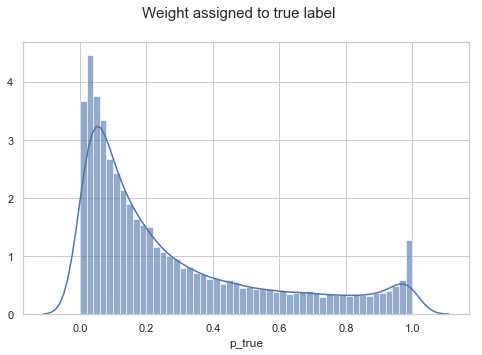
\includegraphics[width=\textwidth]{figures/ptrue-all.png}
\end{figure}

This gives a view of the degree to which the model "committed" to the correct answer, essentially. To put this in context -- if the model were perfect, and always put 100\% of its mass on the right label, we'd just see a single vertical bar at 1.0. So, in the modal case, the model just doesn't really know, and spreads an even ~0.06 of weight on each of the 15 classes. But, we can think of all of the mass to the right of 0.06 as representing meaningful structure learned by the classifier.

Interestingly, though, this varies significantly for individual outlets. Here, the same data, but faceted out for each label:

\begin{figure}[H]
  \centering
  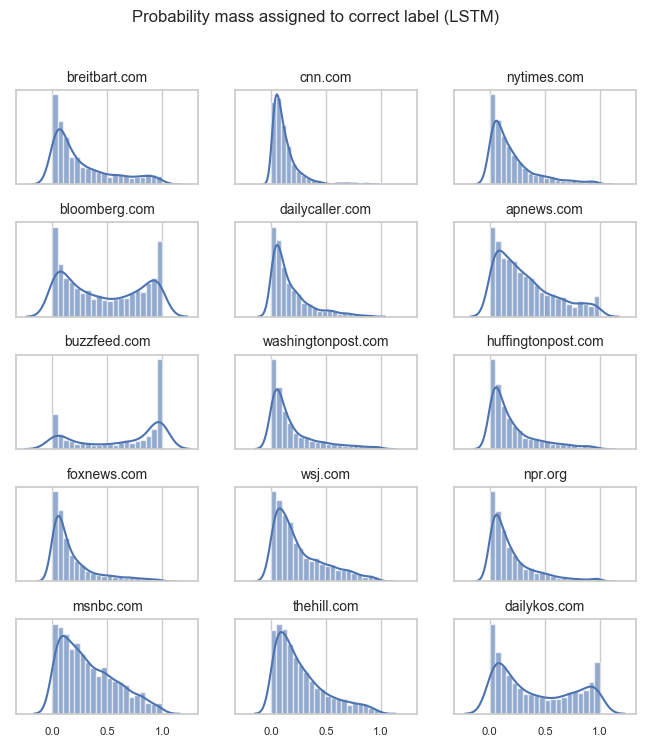
\includegraphics[height=0.5\textheight]{figures/ptrue-multiples.png}
\end{figure}

Where, we can see two basic groups. Bloomberg, BuzzFeed, and Daily Kos all have a spike of very easily-identifiable headlines where the model put ~100\% of its weight on the correct answer. BuzzFeed is the huge outlier -- the model is completely positive a majority of the time.

\begin{figure}[H]
  \centering
  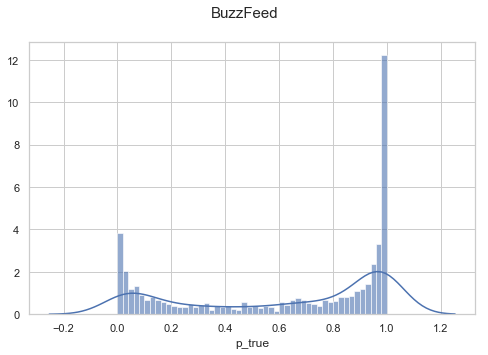
\includegraphics[width=\textwidth]{figures/ptrue-buzzfeed.png}
\end{figure}

Whereas, for CNN -- the model almost never gives more than 0.5 weight to the true label. There are very few headlines, in other words, that are \textit{obviously} from CNN in the eyes of the model.

\begin{figure}[H]
  \centering
  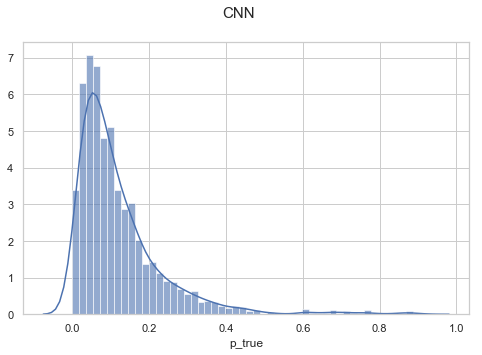
\includegraphics[width=\textwidth]{figures/ptrue-cnn.png}
\end{figure}

But, beyond the performance of the model -- how can we dig into the representations learned by the model, the content of the actual headlines? Under the hood, the raw sentence embeddings produced by the model are 512-dimension vectors, which are hard to make sense of. A simple first step is to project these down to 2 dimensions, which can then be visualized directly. Here, we use UMAP\cite{mcinnes2018umap-software} to transform these into a 2-dimensional embedding, in a way that tries to preserve the relative proximities among the headlines.

\begin{figure}[H]
  \centering
  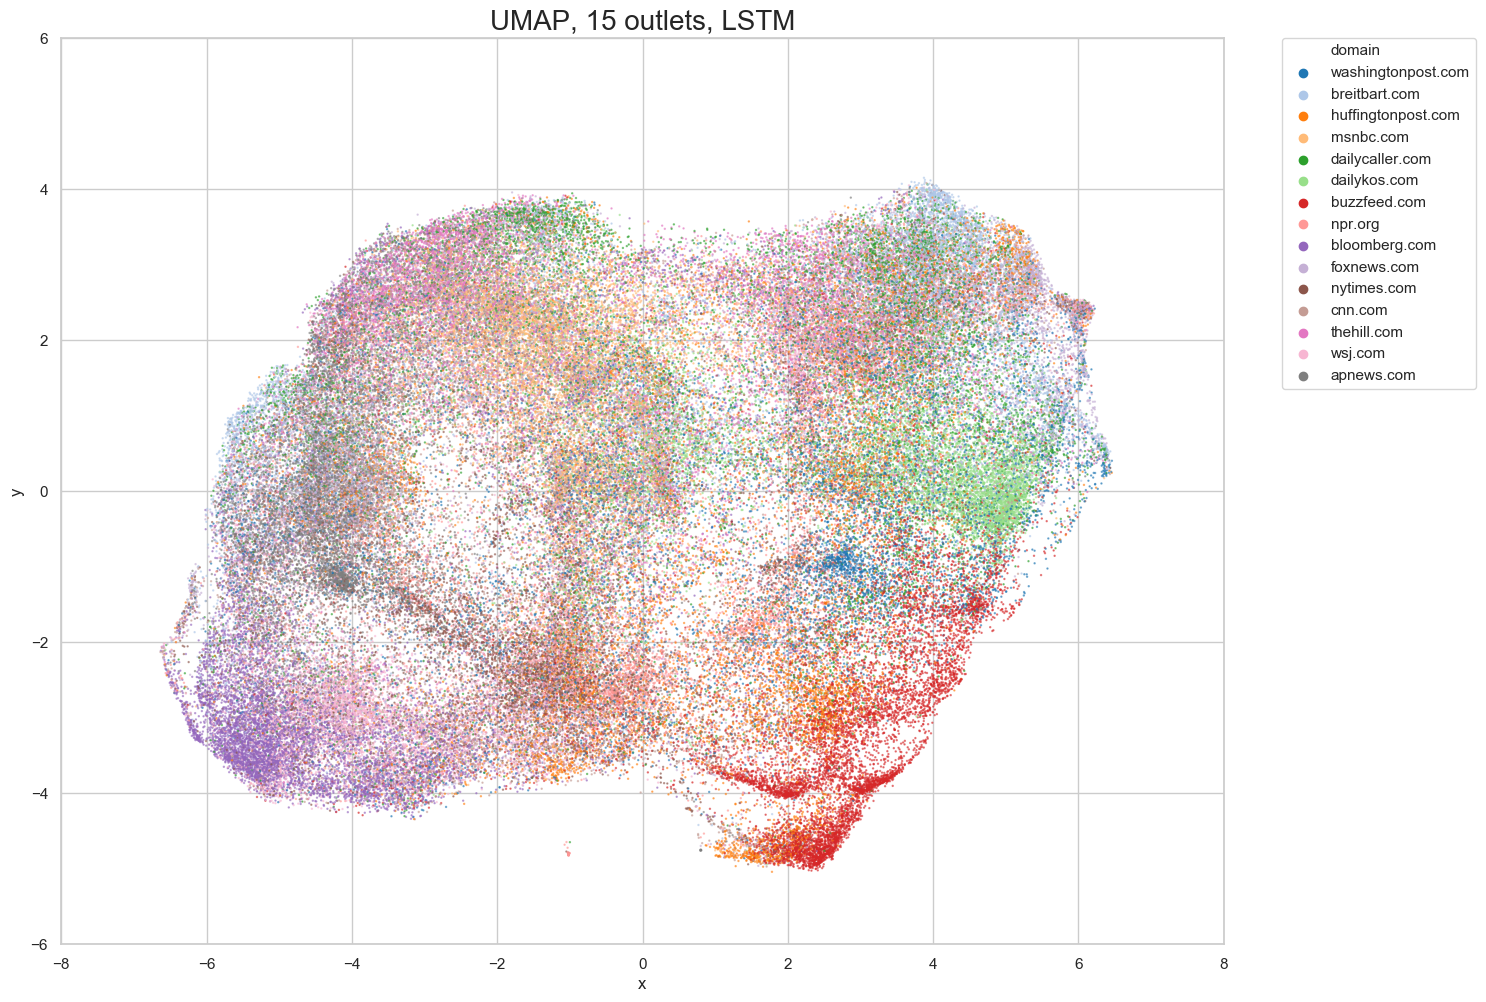
\includegraphics[height=0.8\textheight]{figures/umap.png}
\end{figure}

With everything together, this is a bit hard to make sense of. Foregrounding each outlet individually, we can start to pick out what seem to be coherent "regions" in the projected space:

\begin{figure}[H]
  \centering
  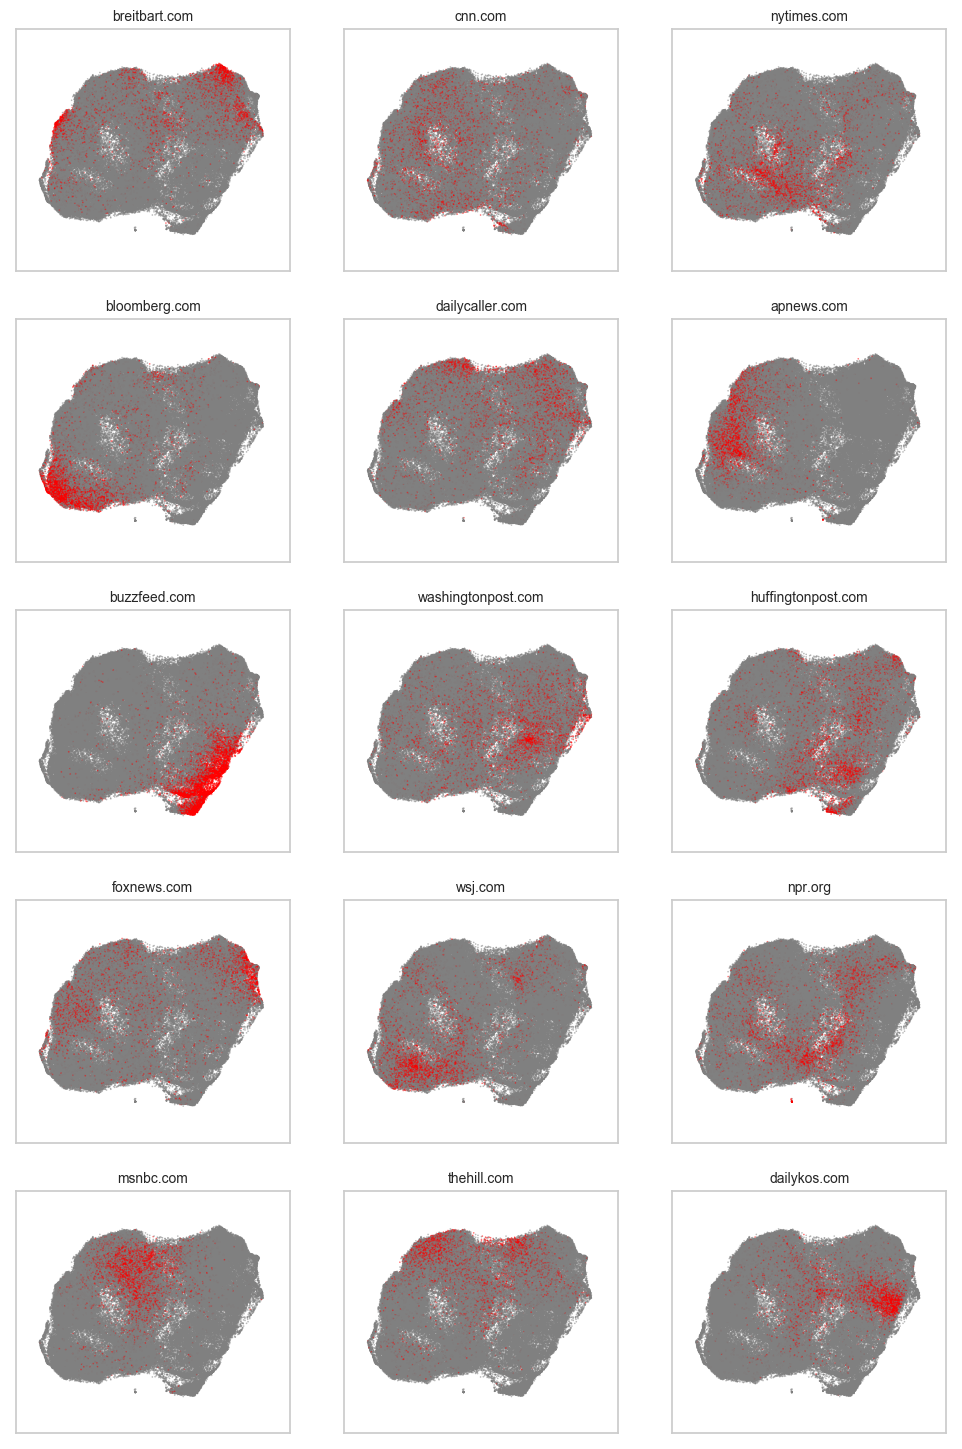
\includegraphics[height=0.8\textheight]{figures/umap-multiples.png}
\end{figure}

Though it's important not to read too much into these types of visualizations, at a high level this suggests that there could be significant differences in the basic "shape" of the embedding space across the different outlets. For example, compare BuzzFeed -- which looks very focused, tightly-packed -- to CNN -- which looks much more scattered and evenly diffused. Or, compare NPR, which, in this projection, seems to have ~2 salient "clusters," to Fox, which has perhaps has 3-4.

There seem to be fairly large differences, in other words, in what might be thought of as the "breadth" or "diameter" of the embeddings in different outlets -- the degree to which the headlines tend to concentrate in a particular region of the linguistic space, or scatter across a larger and more diverse set of topics and styles.

How to be more precise about this? One simple way to measure this is just to look at the \textit{distribution over pairwise cosine distances} for each outlet. At an intuitive level -- if we randomly select two headlines from CNN -- how far apart would we expect them to be? And, how does this compare to the typical distance for The New York Times, Breitbart, BuzzFeed, and so on? Here, we randomly sample (with replacement) 1 million pairs from each outlet, and then build up the distributions over the set of cosine distances between each pair:

\begin{figure}[H]
  \centering
  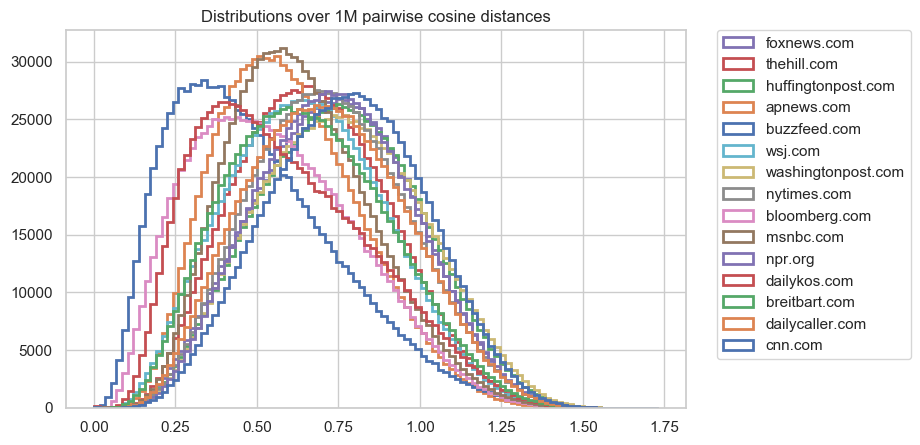
\includegraphics[width=\textwidth]{figures/pwd-hist.png}
\end{figure}

Or, broken out vertically by outlet:

\begin{figure}[H]
  \centering
  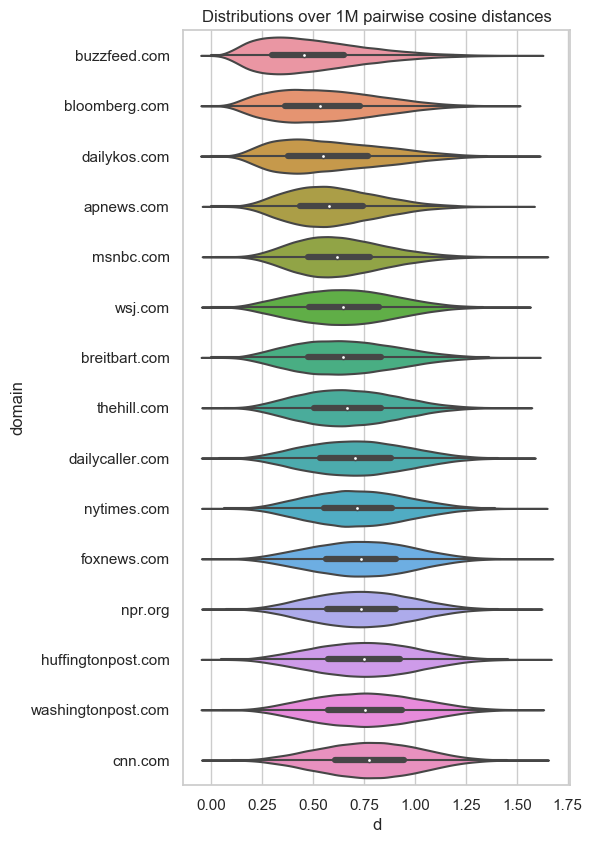
\includegraphics[height=0.6\textheight]{figures/pwd-violins.png}
\end{figure}

We can see differences, then, along two axes. First, the modal value of these distributions varies significantly across the 15 outlets -- smallest for BuzzFeed, at ~0.3, and largest for CNN, at just shy of 0.9. Other very "narrow" outlets include Bloomberg and the Daily Kos, which seems fairly easy to make sense of (Bloomberg is heavy on business and financial reporting; Daily Kos on left-leaning politics); Maybe most surprising is AP, which lands as the third most-focused outlet. (The reasons for this become clearer below, when digging into the internal geometries of the embeddings for each outlet -- basically, AP stories broadly cluster into two nearby clusters, which basically map onto a domestic / international divide.)

Meanwhile, at the other end of the spectrum, along with CNN are Fox, The Washington Post, and NPR are the "widest" or "broadest" outlets. Where, the interpretation is fairly straightforward -- these outlets produce more wide-ranging and diverse headlines; they have less of a "lane," and, at different times, produce content that resembles a number of other outlets.

Another related (though also somewhat different) way of thinking about this is to say that different outlets have different numbers of clusters. Looking at the per-outlet UMAP visualizations, again -- we might say, roughly, that BuzzFeed has 1 cluster; Breitbart has 2-3, depending on how you squint at it; Fox has two groups, one fairly focused and the other more diffuse; CNN seems to be scattered all over the place.

Can we formalize this? Clustering, especially in high dimensions, is kind of a dark art, and it's hard to really produce a definitive result; so all of this should be taken with a grain of salt. But, as an experiment, we can do a basic agglomerative cluster over the embeddings based on pairwise cosine distances, using an "average" linkage rule when deciding whether to join groups. The one hyperparameter here is the cluster merging threshold -- the cosine distance at which, if two (groups of) embeddings are farther apart than this value, they get broken out as flat clusters in the final result. For this value, we simply use the modal value of the complete distribution over pairwise distances, across all outlets (0.63).

\begin{figure}[H]
  \centering
  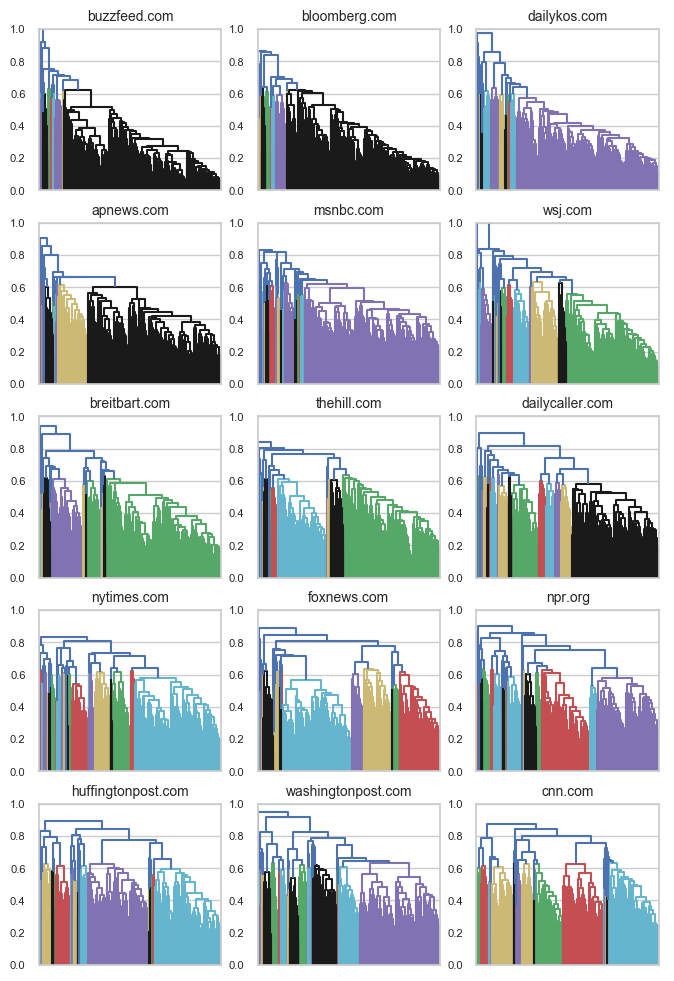
\includegraphics[height=0.6\textheight]{figures/cluster-multiples.png}
\end{figure}

This gives another view on the "shapes" of the outlets. For BuzzFeed and Bloomberg, almost all headlines get put into a single, huge cluster; whereas, for CNN and WaPo, they get spread out over a larger number of more equally-sized clusters.

% TODO: Fox clusters (?)

\section{Modeling the headline graph} \label{section:hl-graph}

So, from digging into the embeddings produced by the neural models, we can get a high-level conceptual "map" of the types of headlines produced by the 15 outlets. But, if the ultimate goal here is to explore the degree to which this structure at the level of language / style / content corresponds (or doesn't) to the underlying audience graph, we need to explicitly model \textit{proximity} or \textit{similarity} -- which outlets are most similar, which are most dissimilar? Or, more precisely -- given a pair of outlets, how can we assign a score that represents the similarity of the headlines from those two outlets, in a way that allows us to compare across the full set of 105 unique pairs of outlets?

Just eyeballing things on the UMAP projection -- some outlets clearly seem to occupy roughly similar regions of the two-dimensional space. For example, Bloomberg and WSJ -- both of which generate a lot of business and financial coverage -- both occupy a significant amount of space in the bottom left of the UMAP projection, around (-6,-4):

\begin{figure}[H]
  \centering
  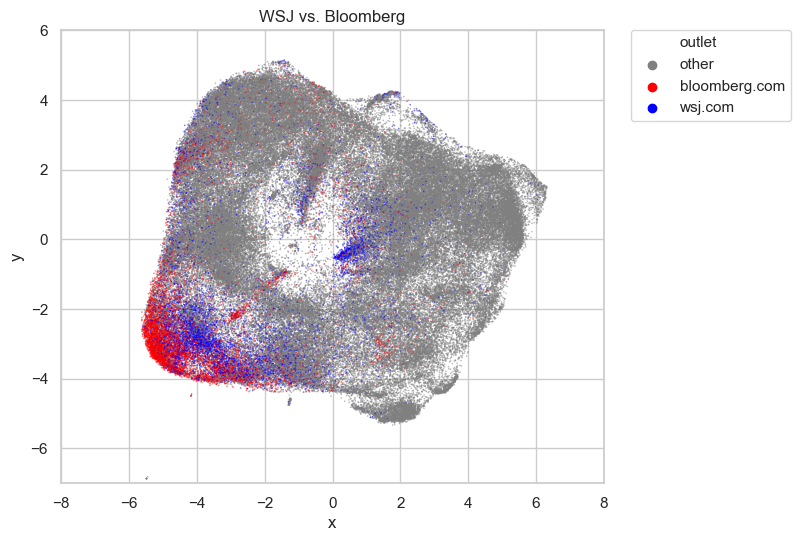
\includegraphics[height=0.4\textheight]{figures/wsj-bloomberg.png}
\end{figure}

How to add precision to this? How can we convert the behavior of the classifiers into a single "score"? Maybe the simplest and most natural way to model similarity, in a predictive setting, is just to look at the confusion matrix -- that is, for each permutation of outlets A and B, the number of headlines from A that the model incorrectly assigns to B. The higher this number, the more "confusable" the two outlets. Using test-set predictions from the LSTM:

\begin{figure}[H]
  \centering
  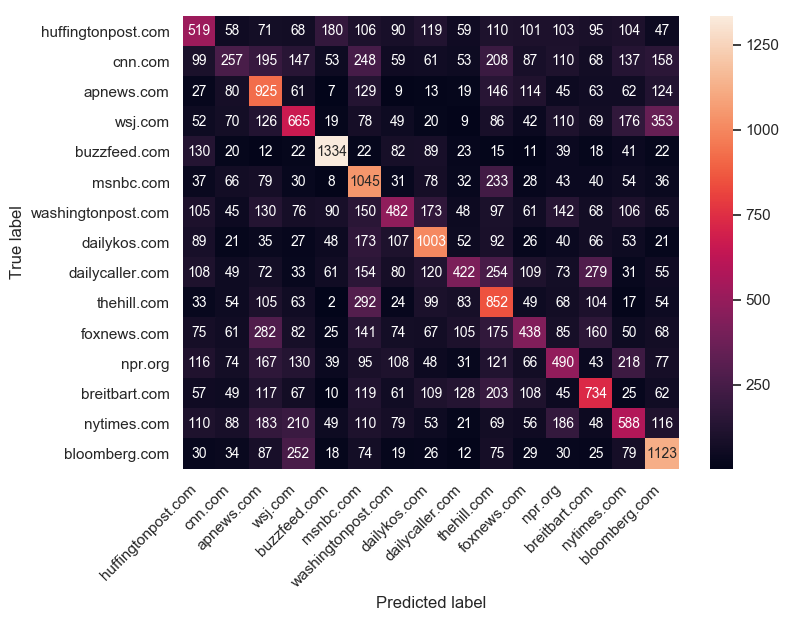
\includegraphics[height=0.4\textheight]{figures/lstm-cm.png}
\end{figure}

Since the class sizes are balanced across the 15 outlets, these counts are directly comparable. So, ignoring the diagonal (where the model is correct), the two most frequently "confused" headlines are from WSJ $\rightarrow$ Bloomberg, where the model makes 320 mistakes; and the two least confused are from AP $\rightarrow$ Daily Kos, where the model makes just 1 mistake. (It's important to note that the confusion counts are \textit{asymmetric} -- eg, the model might misclassify 50 headlines from A as belonging to B, but only 10 headlines from B as belonging to A. So, in building up the set of similarities among the outlets, we need to keep track of the full set of ordered permutations of all pairs.) Skimming off the 10 pairs with the highest and lowest counts:

\begin{figure}[H]
  \centering
  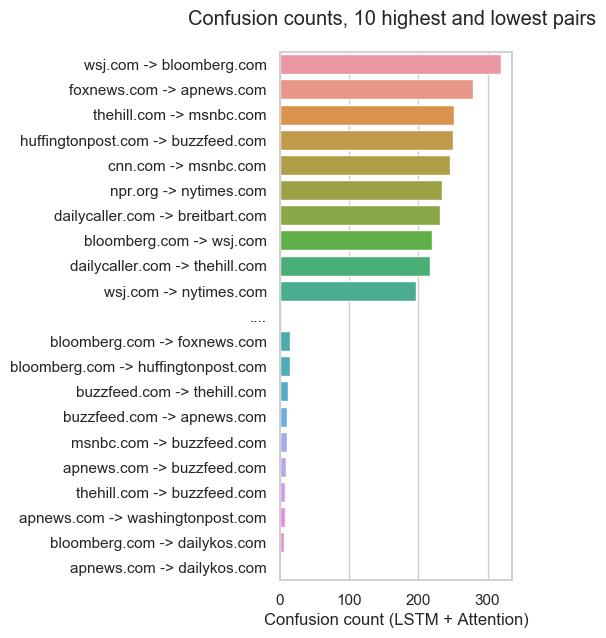
\includegraphics[height=0.4\textheight]{figures/hlg-cc-tb10.png}
\end{figure}

But, this is just one way to do this among many others. For example, instead of counting literal misclassification -- places where the model actually makes an incorrect prediction -- a somewhat more relaxed version of this would be to look at correlations in the assignments of probability mass by the model. For example, if we're comparing WSJ and Bloomberg, we can take the ordered list of probability masses assigned to WSJ for all headlines:

\begin{lstlisting}
[0.00619, 0.17596, 0.03041, 0.01991, 0.00007, 0.01776, 0.01682, 0.00010, 0.00626, 0.09664 ...]
\end{lstlisting}

And the the probability masses assigned to Bloomberg for the same headlines:

\begin{lstlisting}
[0.00279, 0.49098, 0.00894, 0.00222, 0.00005, 0.00449, 0.00378, 0.00012, 0.00284, 0.02261 ...]
\end{lstlisting}

And then just calculate the correlation between these two sets of weights -- when the model puts more weight on WSJ, does it also tend to put more weight on Bloomberg? We can't directly compare these correlations to the confusion counts, since the units are different -- probability masses vs. counts. But, we can simply standard-scale them -- subtract out the mean, scale to unit variance -- and then compare the adjusted scores. Here, the confusion counts alongside Pearson, Spearman, and Kendall-Tau correlations on the probability masses, again skimming off the 10 strongest and weakest pairs:

\begin{figure}[H]
  \centering
  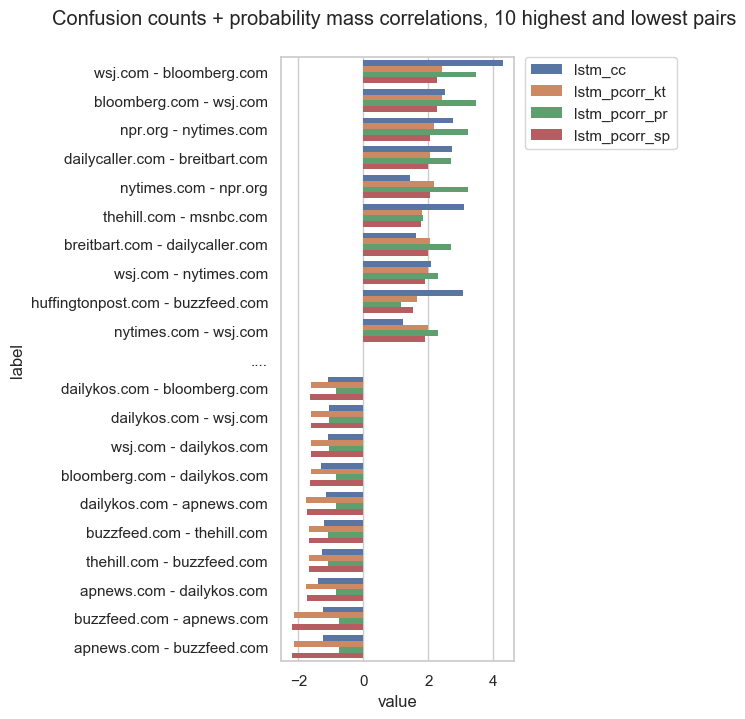
\includegraphics[height=0.4\textheight]{figures/hlg-cc-pcorr-tb10.png}
\end{figure}

So, these generally correlate, though far from perfectly. For example, with the HuffPo $\rightarrow$ BuzzFeed comparison -- the confusion count is ~3 standard deviations above the mean for all pairs, but the Pearson correlation over the probability mass assignments is just over 1 standard deviation above the mean.

Why the difference? Is one more "true" or "real"? This is debatable, but probably the least wrong thing is to say that they operationalize different types of similarity. For example, thinking about the classifier graphically, as a decision boundary in a 2-dimensional space -- the high confusion counts mean that there are a large number of headlines (relative to other pairs) that sit very close to (and just on the wrong side of) this boundary. But, this doesn't tell us anything about the rest of the headlines. For example, it could be that a large majority of headlines from both outlets are very far from the decision boundary -- the outlets are generally very distinctive -- but that there is a particular subset of headlines, maybe about one particular topic, that happen to be very difficult for the model to tell apart. In which case, the probability correlation might seem like a better metric -- it might capture the fact that, overall, the outlets focus on significantly different types of coverage, and not get swayed as much by the minority of headlines that look very similar.

But, in other cases, the probability correlation might seem misleading. For example, it's conceivable that there could be a pair of outlets could have a very high level of linear correlation in assigned probability mass in the context of a multiclass model -- when A seems more likely, so does B, in general -- but that, on a head-to-head basis, the model almost never actually confuses them for each other.

The point being -- for almost any metric, we can imagine both ideal and pathalogical cases, situations where that particular formulation of similarity seems either very good or very bad. "Similarity" is fundamentally complex, especially in a case like this where the things being compared are actually large, heterogeneous aggregations over individual headlines.

Yet another approach to this -- so far, we've been training models under a multiclass objective -- the model is handed a headline, and makes a prediction across all 15 outlets. But, we could also formulate this as a large battery of completely independent, A-vs-B comparisons -- NYT vs WSJ, NYT vs. Bloomberg, NYT vs. Breitbart, and all other 117 unique combinations that can be formed from the 15 outlets. As long as the training samples are size-balanced across all pairs, so that they always see exactly the same number of headlines from each outlet -- we can directly compare the classification accuracies from these binary models. Because of resource constraints, it's not feasible to re-train the strongest neural models on pairwise samples (which are very slow without GPUs, and we don't currently have access to massively parallel GPU compute). But, the non-neural baselines, which are only a few percentage points off the neural models in the multi-class benchmark, can be fit very efficiently on standard CPUs, which makes it possible to parallelize these models across thousands or even millions of separate comparisons using commodity cloud hardware.

For example, using the linear SVC, the stronger of the two non-neural baselines -- we can take all 105 unique pairwise combinations from the 15 outlets, and, for each pair, fit 100 models on randomly sampled headlines for that pair. For example, for the first comparison -- say, NYT vs. WSJ -- we would sample 18k headlines from NYT, 18k from WSJ, break these 36k headlines on an 80/20 train-test split, fit a model, and evaluate the accuracy on the test set. And then, do this 99 more times for NYT vs. WSJ, each time sampling a new random subset of 18k/18k headlines. For all 105 pairs, this gives a total of 10,500 independent model fits, all of which are totally independent of each other, and can be easily parallelized -- here, using Spark, on a 320-core cluster on AWS, which can run this in about an hour. We can then use these 10,500 accuracy scores to form very tight confidence interval over the pairwise accuracies for each comparison (Figure \ref{svc-ab-acc}).

\begin{figure}
  \centering
  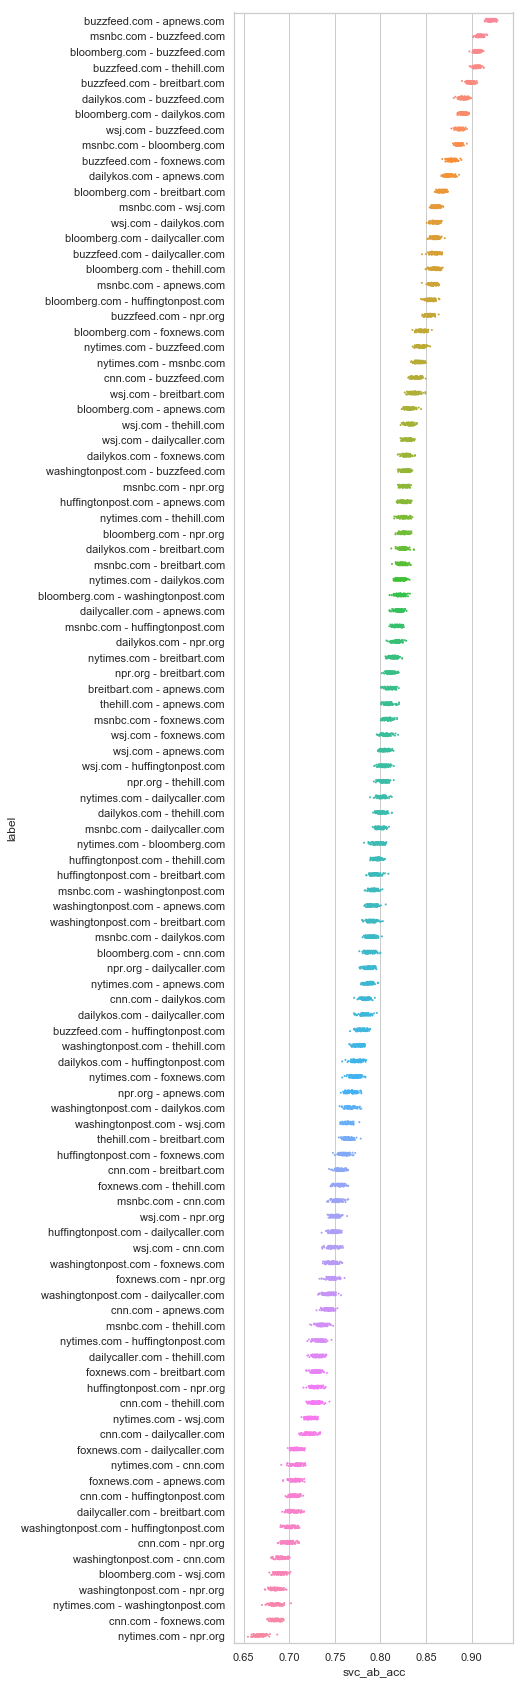
\includegraphics[height=\textheight]{figures/svc-ab-acc.png}
  \caption{Pairwise SVC accuracies on size-balanced samples, 100 models per pair.}
  \label{svc-ab-acc}
\end{figure}

These per-pair scores can simply be averaged, to get a set of 105 scores, which can then be scaled to zero mean and unit variance and plugged in with the previously developed scores:

\begin{figure}[H]
  \centering
  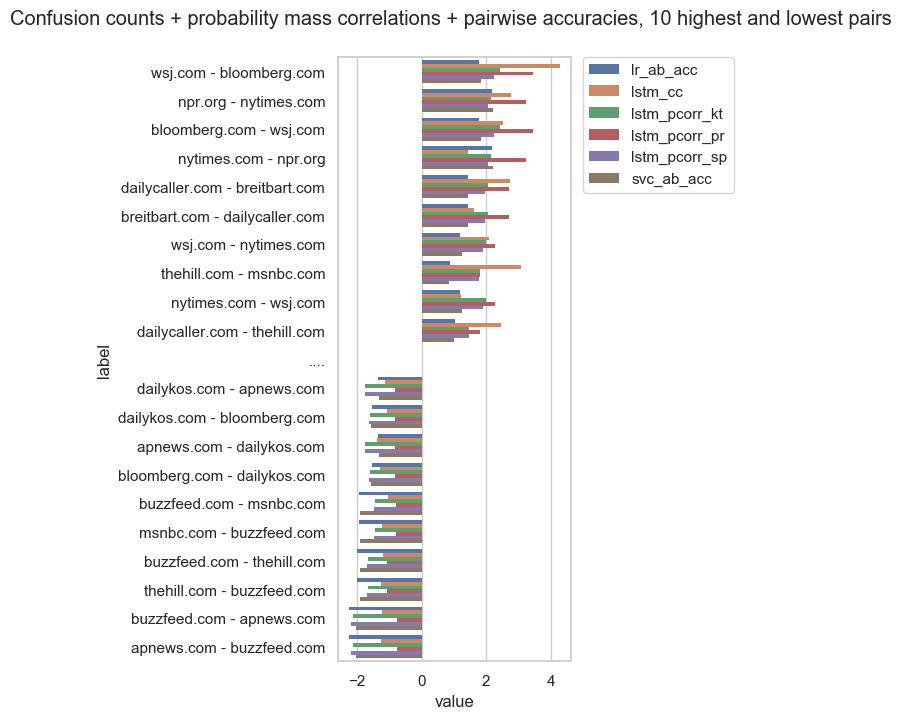
\includegraphics[height=0.4\textheight]{figures/hlg-cc-pcorr-acc-tb10.png}
\end{figure}

(With the classification accuracies, to make them comparable with the confusion counts and mass correlations, we simply flip the signs on the scaled scores, since a high accuracy corresponds to low similarity.)

Which, we can see, are broadly converging. By taking a battery of different similarity metrics, we can triangulate across a wide range of different modeling decisions and be sure that the final results are durable, regardless of which of these different measuring tapes we use.

So, what does the full set of available metrics look like? There's a kind of combinatorial explosion of possibilities, but, for the purposes of this analysis, we use:

\begin{itemize}
\item Confusion counts and probability correlations (Pearson, Spearman, Kendall-Tau) for the three major neural architectures -- LSTM, CNN, and CBOW.
\item Confusion counts and classification accuracies from pairwise SVC and logistic models.
\end{itemize}

Which gives a total of 16 different representations of headline similarity for each pair of outlets. Then, joining all of these together and applying standard scaling, we can represent the similarity between each pair of outlets as a collection over these 16 independently calculated scores:

\begin{figure}[H]
  \centering
  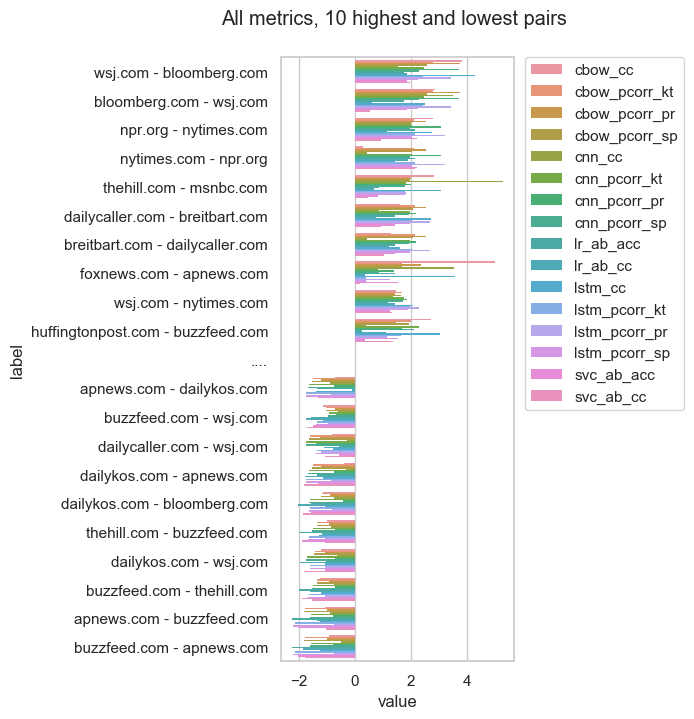
\includegraphics[height=0.4\textheight]{figures/hlg-all-tb10.png}
\end{figure}

And, averaging over the metrics, and converting into a literal graph -- here, for visual clarity, collapsing the bidirectional edges into a single undirected edge, averaging over the two scores:

\begin{figure}[H]
  \centering
  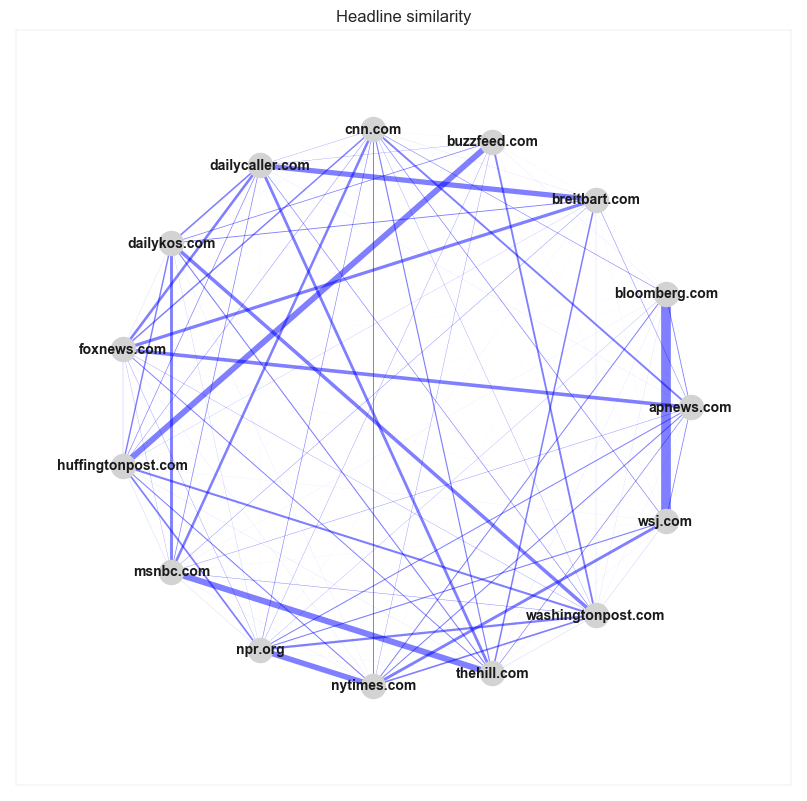
\includegraphics[height=0.5\textheight]{figures/hl-graph-radial-all-metrics.png}
  \caption{Pairwise headline similarities, averaging across all metrics and both directions for each pair. To make it easy to see the strongest pairs, in this figure the edge weights are mapped to a 0-1 scale and then cubed.}
\end{figure}

So -- WSJ / Bloomberg take the cake for the single strongest link, followed by NPR / NYT, The Hill / MSNBC, and Daily Caller / Breitbart.

\section{Modeling the audience graph}

So, from the classifiers -- a fully connected graph out news outlets, where the edge weights represent the degree to which headlines from each pair of outlets are similar or different. To return to original question -- how does this graph compare to the underlying audience graph, the social graph of users on Twitter who distribute the content? For example, to WSJ and Bloomberg also have the highest correlation at the level of audience, from among all the pairs of outlets?

Measuring similarity between the outlets at the level of the headlines was relatively complex. But, in many ways, measuring the audience similarity is more straightforward, especially in the context of social media platform like from Twitter, where every individual tweet is associated with a stable user id. From these, we can trivially assemble the set of unique users who has ever tweeted a link to a \texttt{nytimes.com} URL, a \texttt{wsj.com} URL, a \texttt{breitbart.com} URL, etc.

And, unlike with the headlines, where we had to do quite a lot of work before we could say that a headline from outlet A is "confusable" for a headline from B -- with the social graph on Twitter, users have literal multiple-membership relationships with the different outlets, baked natively into the raw data. A single user can be unambiguously associated with more than one outlet -- by tweeting a link, following an account, etc -- whereas, with the headlines, a single headline can only "belong" to a single outlet, and we needed to develop an elaborate machinery from scratch to measure similarity (the classifiers).

Again, there are various ways to do this, but we stick with something simple -- just calculate correlations in link counts across the 15 domains at the level of individual user accounts. For example, imagine we just had 3 outlets -- NYT, NPR, and CNN -- and two users, 1 and 2. If user 1 has tweeted 10 links to NYT, 5 to NPR, and 3 to CNN, we'd represent this as:

\begin{lstlisting}
[10, 5, 3]
\end{lstlisting}

And, if user B has tweeted 2 links to NYT, 20 to NPR, and 5 to CNN, we'd have:

\begin{lstlisting}
[2, 20, 5]
\end{lstlisting}

These count vectors can be assembled for all 8M users who have ever tweeted at least one link to any of the 15 analysis domains. Then, from these, we can calculate correlations between the counts for all unique pairs of domains -- which gives, for each pair, the degree to which users tend to share links from both of them. Thinking of it as a huge actor / count matrix, just take correlations over all pairs of columns, each of which represents one of the outlets. Here, like before, we tabulate the Pearson, Spearman, and Kendall-Tau correlations for each pair of outlets. Here, sorting by the Kendall-Tau correlation:

\begin{figure}[H]
  \centering
  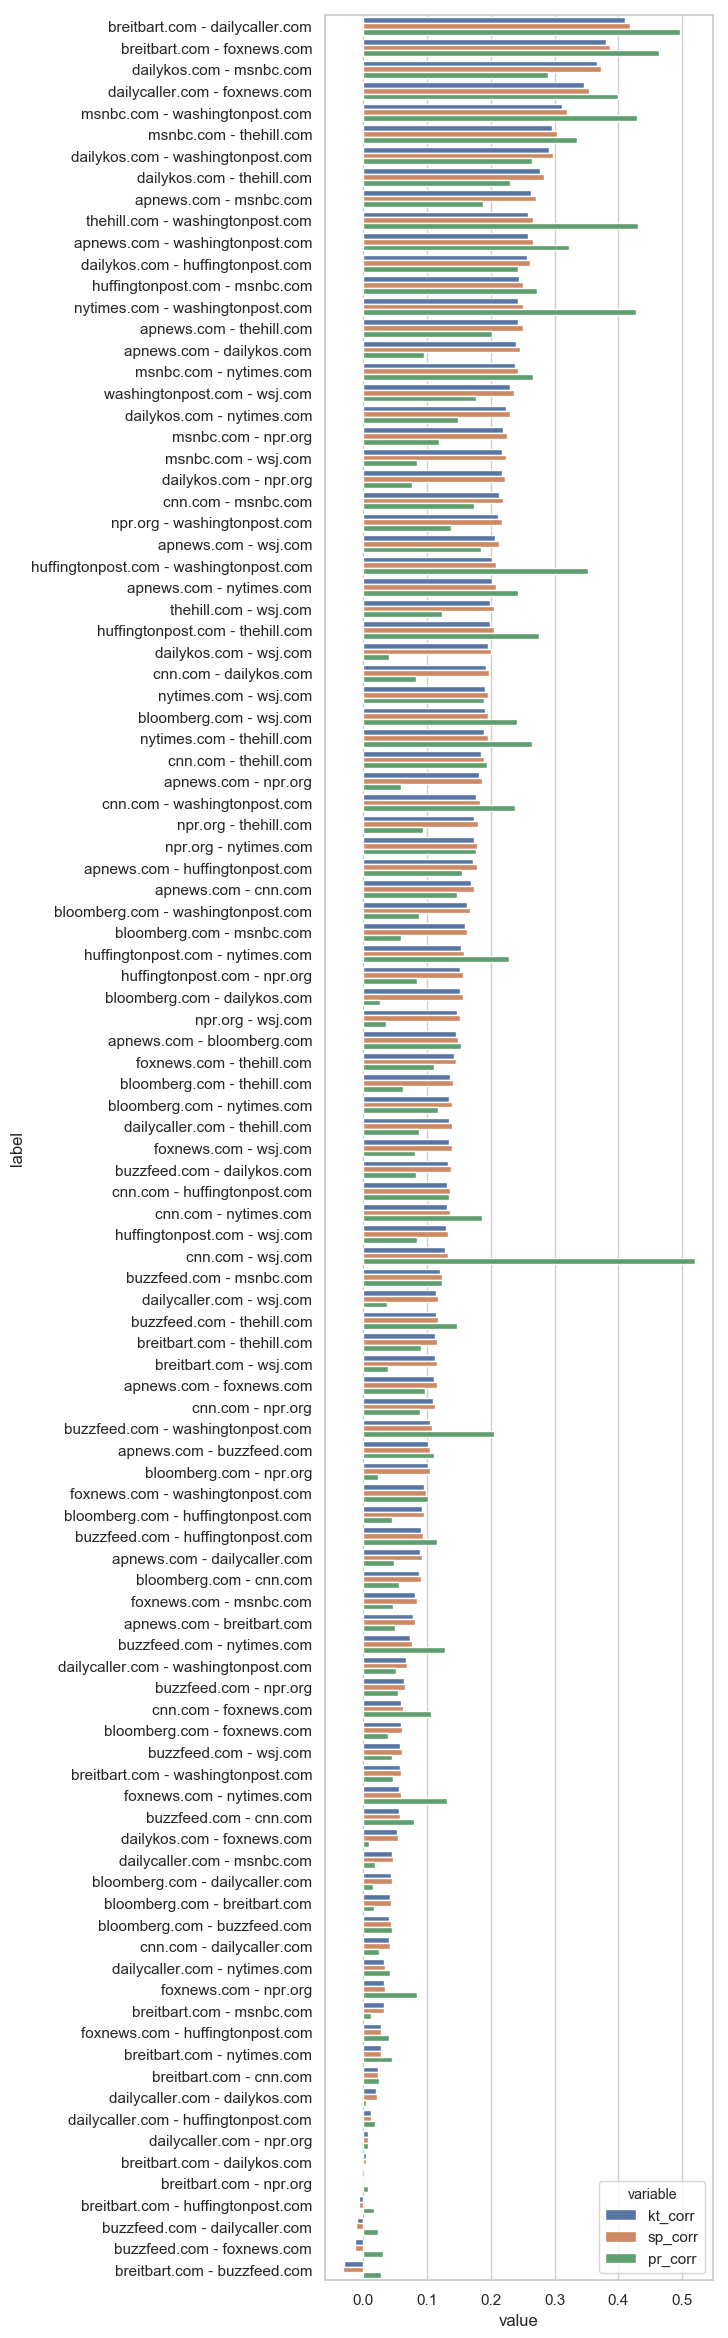
\includegraphics[height=0.4\textheight]{figures/user-graph-bars-all.png}
\end{figure}

Overall these paint a fairly consistent picture, with Breitbart and Daily Caller as the most highly audience-correlated outlets under all three metrics. Though, there are places where the Pearson correlation diverges significantly from the Spearman and Kendall-Tau -- especially with CNN / WSJ, where the Pearson correlation is extremely high, but Spearman and Kendall-Tau are middling. This is a function of the fact that Spearman and Kendall-Tau are based on the rank-ordering of the counts, whereas Pearson operates on the actual counts; and, here, there's clearly a small set of users (or even just a single user) that have posted an \textit{extremely} large number of links from both CNN and WSJ, which has the effect of cranking up the overall Pearson correlation.

Indeed, looking more closely at the number of links posted by each user, we can see that this distribution is highly skewed -- out of 8.1 million users, 5.5 million (68\%) have only posted a single link. And, a handful of users have posted a \textit{massive} number of links -- 23 users have over 10,000 links. (These are likely organizational accounts or bots.)

\begin{figure}[H]
  \centering
  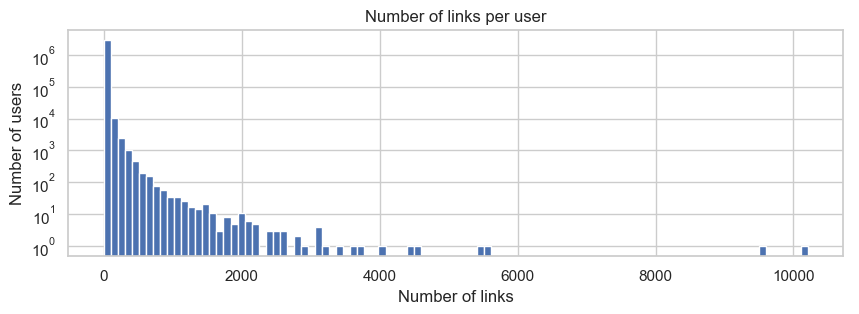
\includegraphics[width=\textwidth]{figures/links-per-user.png}
\end{figure}

To be sure that these two extremes -- "undersampled" accounts that only appear a handful of times, and "oversampled" accounts that are incredibly prolific -- aren't skewing the relationships in problematic ways, we can calculate a second set of correlations for each pair of outlets, but this time just considering users who appear between 10 and 100 times in the dataset. Here, the same set of 3 correlation metrics:

\begin{figure}[H]
  \centering
  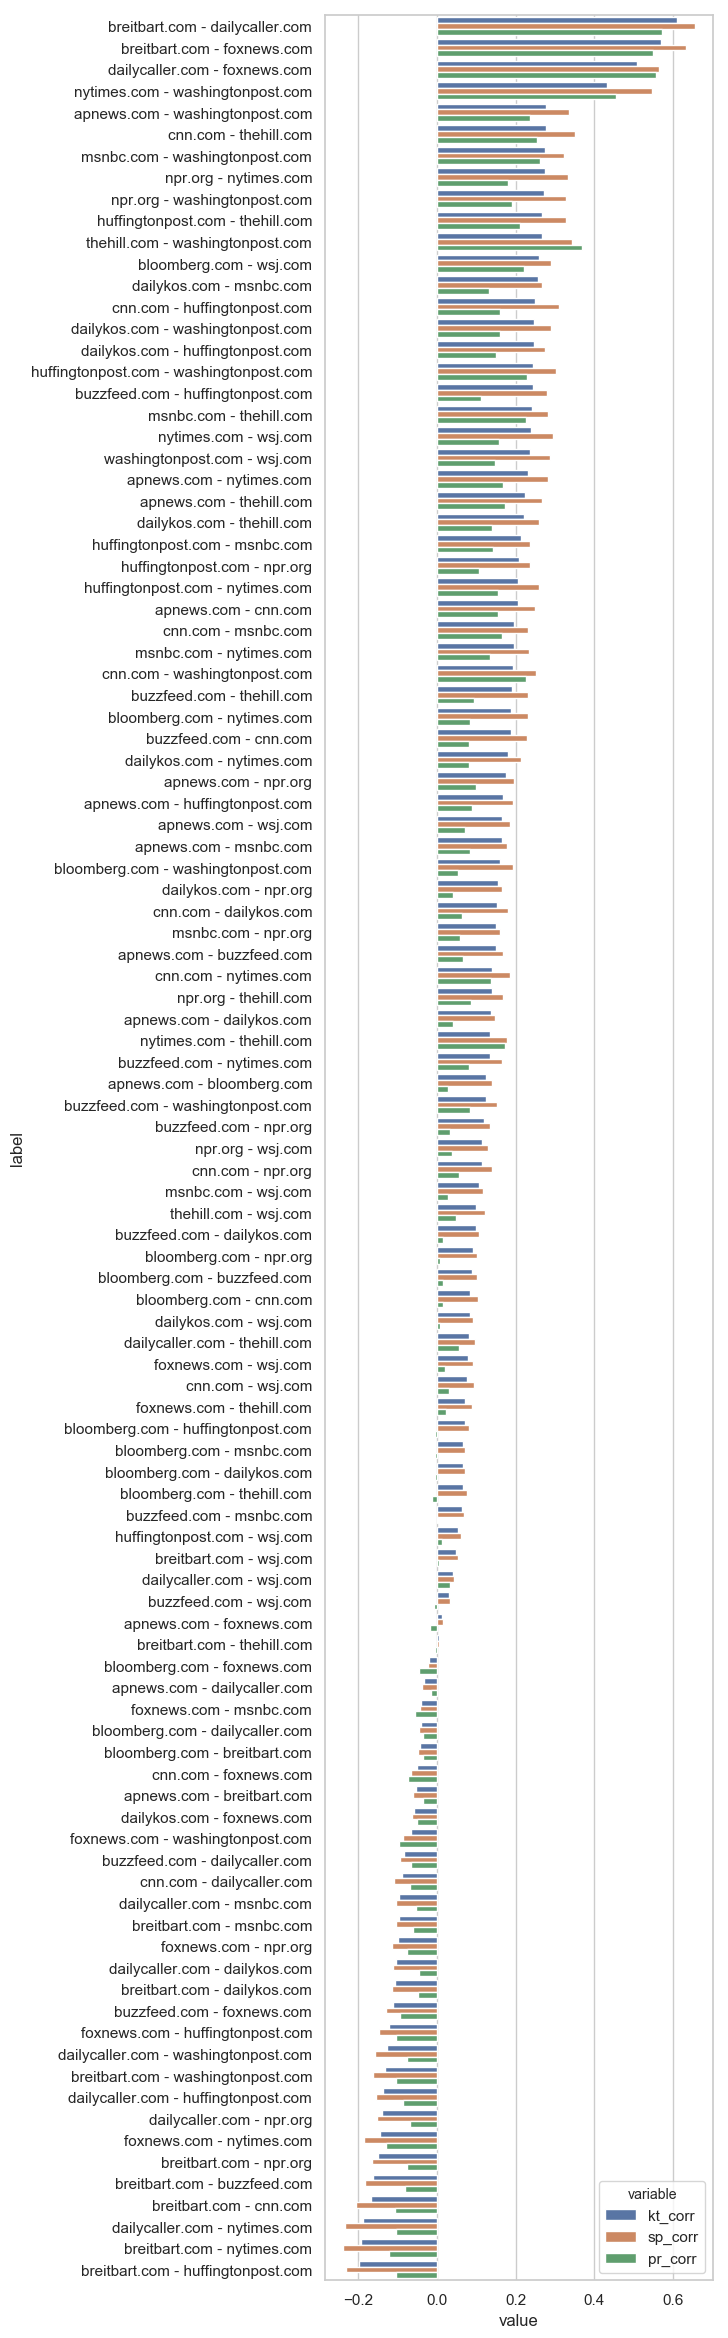
\includegraphics[height=0.4\textheight]{figures/user-graph-bars-10-100.png}
\end{figure}

Like with the headlines, the idea here is to pull out a "grid" of measurements using different techniques and hyperparameters, to be sure that we don't over-interpret a noisy or idiosyncratic result from a single type of measurement. Here, as a literal graph, with the edge weights based on the average score for each pair:

\begin{figure}[H]
  \centering
  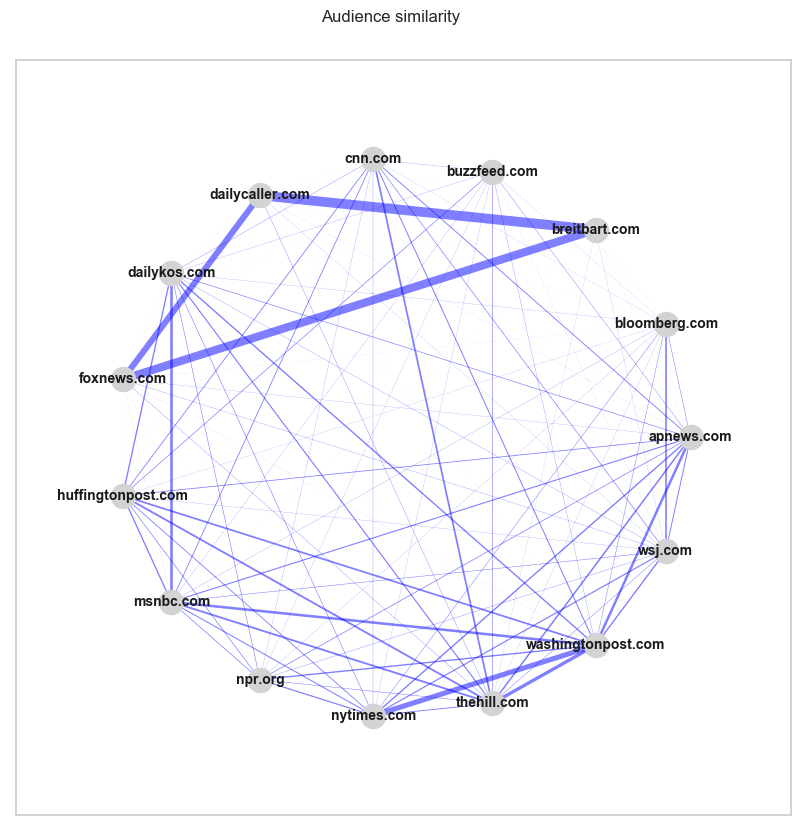
\includegraphics[height=0.5\textheight]{figures/user-graph-radial-all-metrics.png}
  \caption{Pairwise audience similarities, averaging across all metrics and both directions for each pair. To make it easy to see the strongest pairs, in this figure the edge weights are mapped to a 0-1 scale and then cubed.}
\end{figure}

\section{Headlines vs. audience} \label{section:content-audience}

At this point, we've got all the raw ingredients in place to start to explore the question of how similarities at the level of content correspond (or don't correspond) to similarities at the level of audience. To recap -- we've induced two sets of weights over the 15 outlets, one representing similarity at the level of headlines, and the other representing correlations in the set of users who tweet the content:

\begin{figure}[H]
\centering
\begin{subfigure}{.5\textwidth}
  \centering
  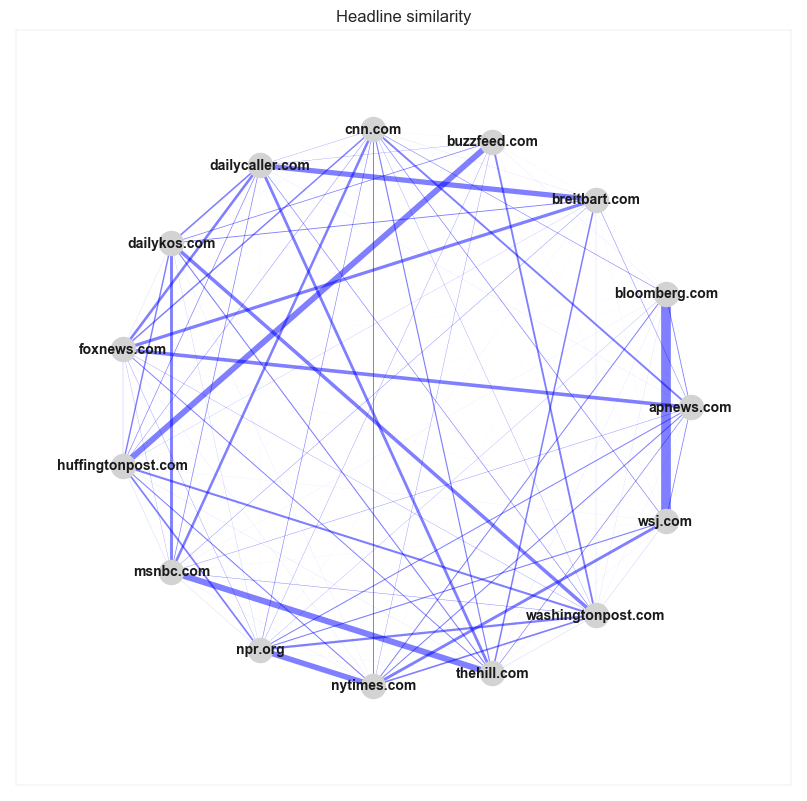
\includegraphics[width=0.8\linewidth]{figures/hl-graph-radial-all-metrics.png}
  % \caption{Scaled headline similarity scores.}
  % \label{fig:sub1}
\end{subfigure}%
\begin{subfigure}{.5\textwidth}
  \centering
  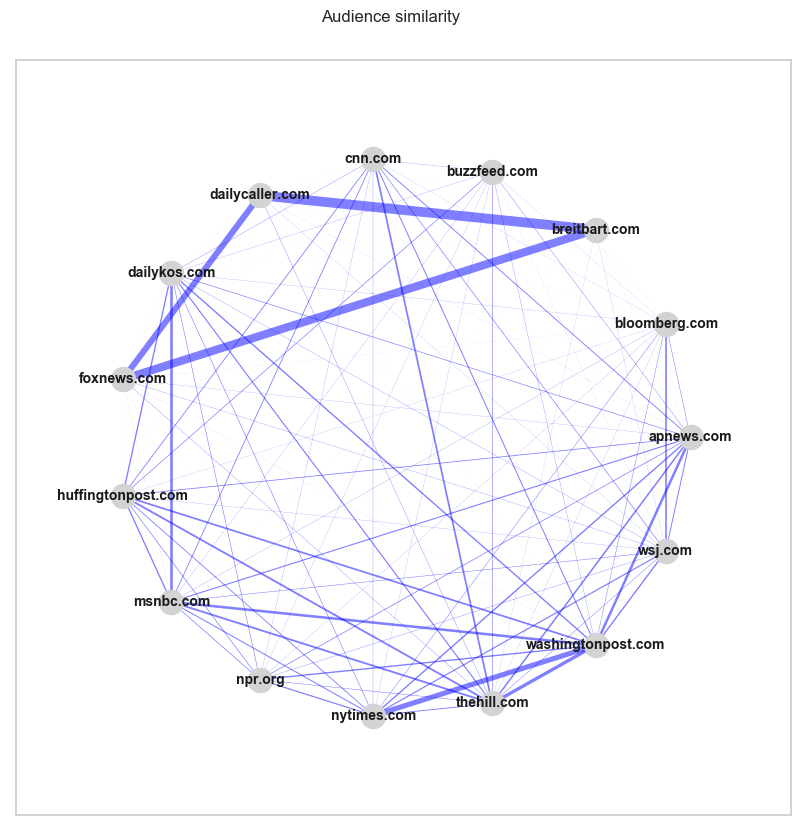
\includegraphics[width=0.8\linewidth]{figures/user-graph-radial-all-metrics.png}
  % \caption{Scaled audience similarity scores.}
  % \label{fig:sub2}
\end{subfigure}
\caption{Scaled headline and audience similarities.}
% \label{fig:test}
\end{figure}

Zooming down to the level of an individual outlet, for example, The New York Times -- we can represent the full linguistic "signature" of NYT as a set of pairwise scores with all other outlets, where each score is actually a family of individual metrics that represent different ways of modeling the linguistic similarity. So, for example, for the LSTM Kendall-Tau probability correlations (\texttt{lstm\_pcorr\_kt}), we get 14 values, each representing the linguistic similarity between NYT and one of the other outlets. These 14 scores are then normalized to zero-mean and unit-variance, which makes it possible to compare across measurements with different units. So, here, we can see that NYT is most similar to NPR, when averaged across all metrics, and least similar to The Hill:

\begin{figure}[H]
  \centering
  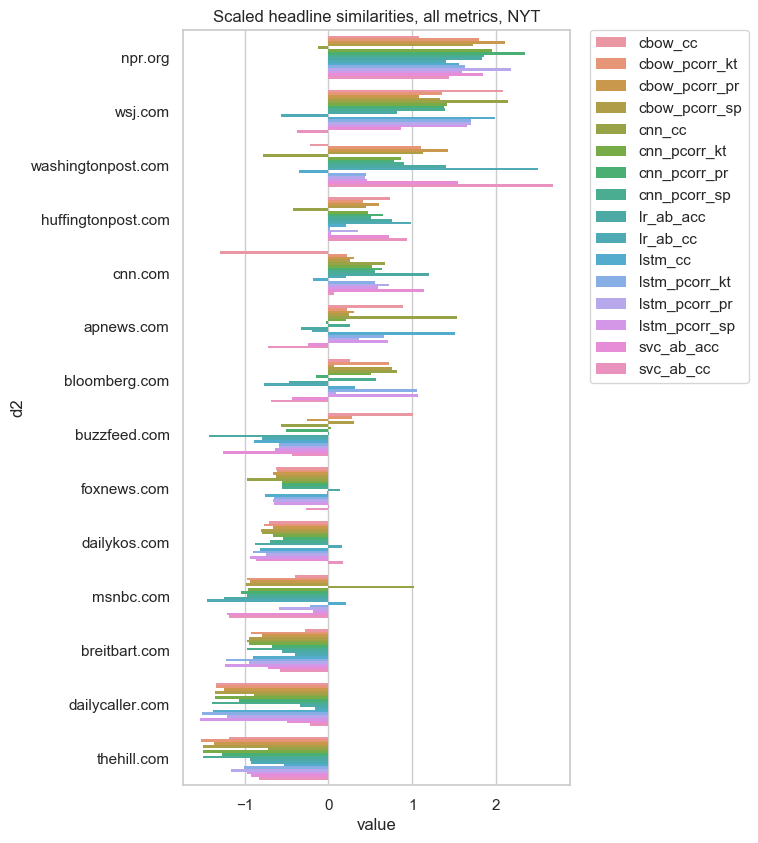
\includegraphics[height=0.5\textheight]{figures/ca-nyt-content.png}
\end{figure}

Meanwhile, parallel to this -- for the headline graph, we get a second set of pairwise similarities at the level of audience. So, the NYT audience correlates most closely with The Washington Post, and least closely with Breitbart:

\begin{figure}[H]
  \centering
  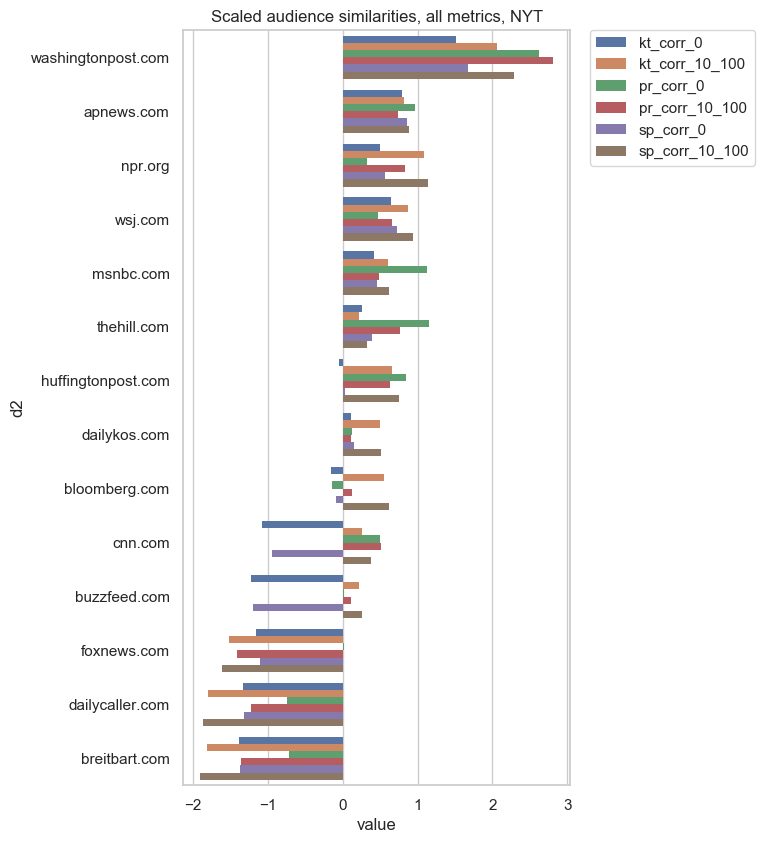
\includegraphics[height=0.5\textheight]{figures/ca-nyt-audience.png}
\end{figure}

With these two sets of similarities in place, we can now simply ask -- to what extent do these two sets of weights correlate with each other? For example, when NYT is similar to NPR in terms of the content of headlines -- is it also similar at the level of audience, is there also a high level of correlation between the set of users who tweet links to NYT and users who tweet links to NPR?

To make the comparison clearer, we can stack the two sets of weights on top of each other. Here, the headline similarity metrics for each (NYT, other) pair are rolled together into the blue bars, and the audience similarities are averaged into the orange bar. Then, we sort by headline similarity:

\begin{figure}[H]
  \centering
  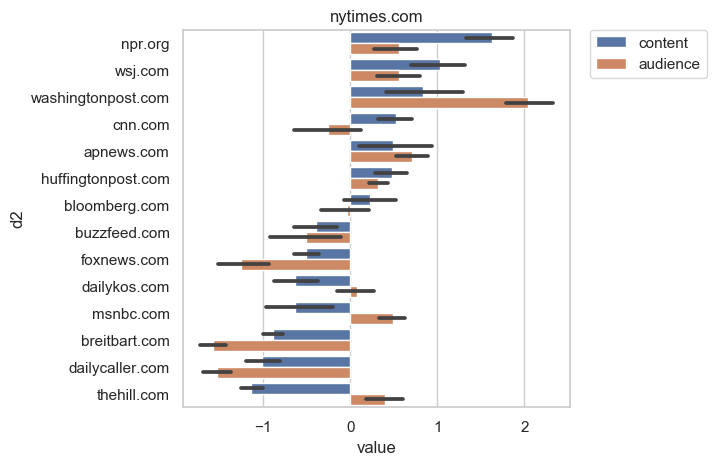
\includegraphics[width=\textwidth]{figures/ca-nytimes-composite.png}
\end{figure}

Which makes it possible to see the overall level of alignment between the two sets of weights. Generally, the correlation between headlines and audience is fairly tight; though, we can see a couple of places where this breaks down. Namely, NYT has very low headline overlap with The Hill -- in fact, the \textit{lowest} out of all 14 of the other outlets -- but a relatively high overlap at the level of audience. Also notable is the fairly large disconnect with NPR -- NYT is closer-than-average to NPR for both content and audience, but by a significantly larger margin for audience than for content -- NYT headlines "sound" very similar to NPR headlines; but the audience correlation is just a bit above average for the NYT.

For NYT, then -- an alignment between content and audience, though with a couple of wrinkles. How can we quantify this? Under the hood, for each combination of \texttt{(NYT, other outlet)}, we've got 16 different headline similarity scores and 6 different audience similarity scores. From these, we can take each unique pairing of headline metric and audience metric and simply calculate the correlation of these scores, across each of the other 14 outlets. This gives, then a \textit{distribution} over correlations that represent the degree to which the NYT headline graph matches up with the NYT audience graph:

\begin{figure}[H]
  \centering
  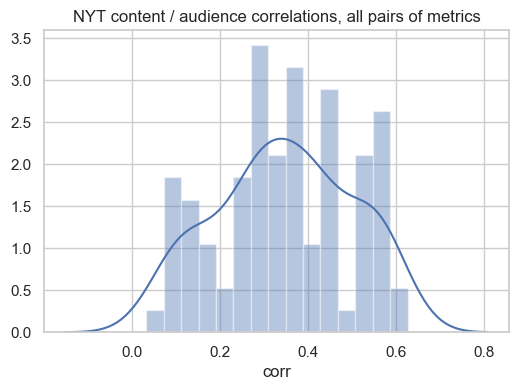
\includegraphics[width=0.6\textwidth]{figures/nyt-corr-dist.png}
\end{figure}

So, a modal value of ~0.3, though with quite a bit of variation. (This is where the collection different measurements of similarity come in handy -- by aggregating over all of them, we can get a much more densely-sampled view on these relationships.) We can then do this for each of the 15 outlets, and compare these distributions over correlations, which surfaces some significant differences:

\begin{figure}[H]
  \centering
  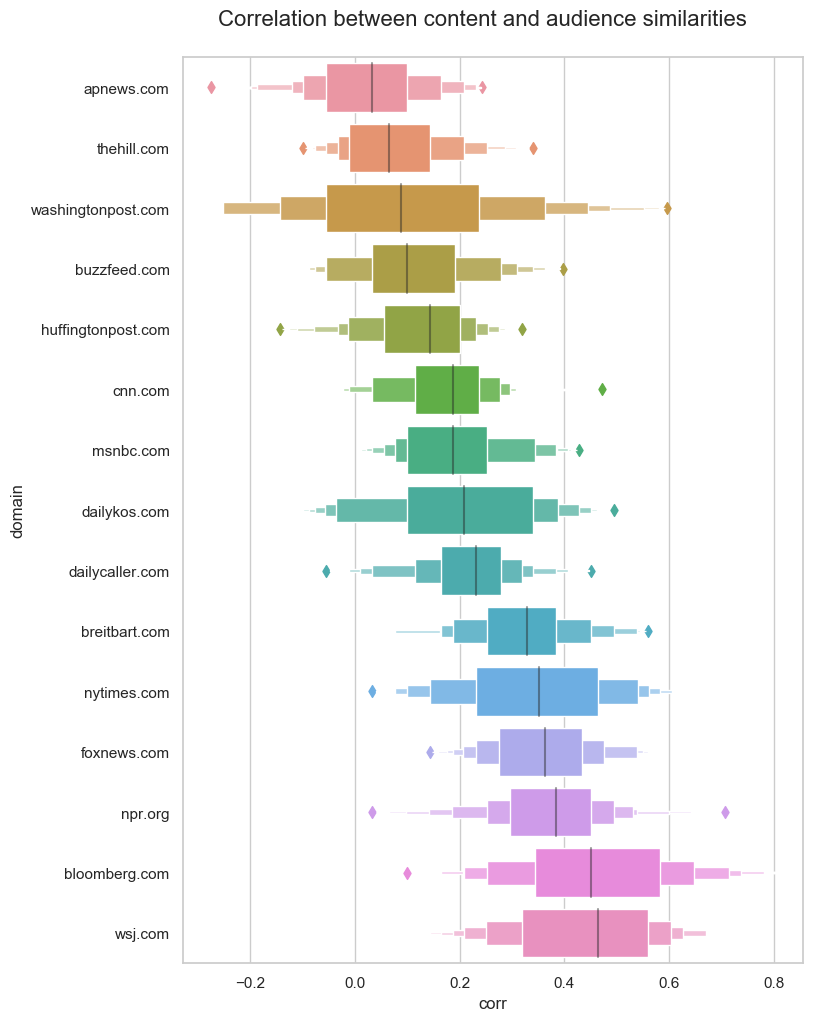
\includegraphics[height=0.7\textheight]{figures/ca-corr.png}
\end{figure}

Overall, then, content similarity tends to correlate positively with audience similarity. But, the individual outlets spread out fairly smoothly between 0 and 0.5. At the high end of this range -- WSJ and Bloomberg occupy very similar "locations" in the headline and audience graphs -- when WSJ "sounds like" another outlet, it generally also has a very high level of audience overlap with the outlet. To get a sense of what this looks like -- here are the broken-out content / audience similarities for these two:

\begin{figure}[H]
  \centering
  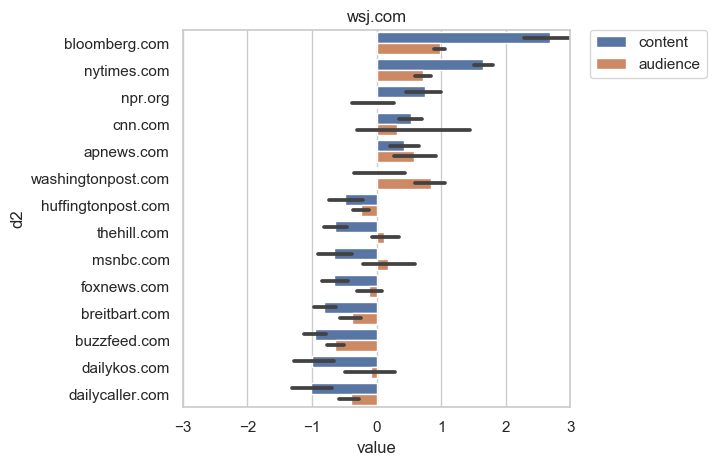
\includegraphics[width=\textwidth]{figures/ca-wsj-composite.png}
\end{figure}

\begin{figure}[H]
  \centering
  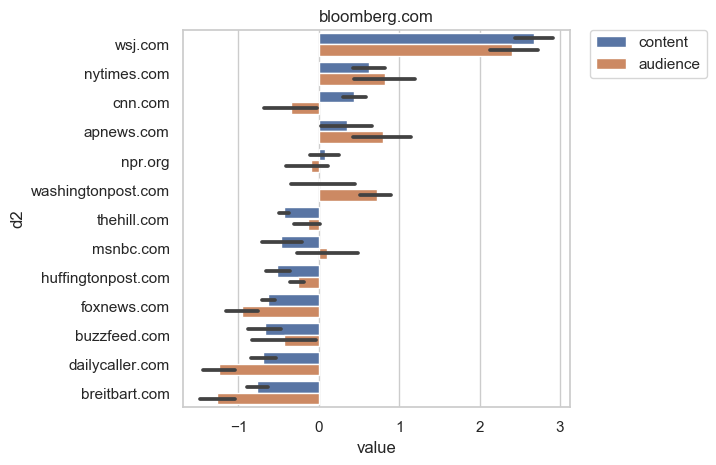
\includegraphics[width=\textwidth]{figures/ca-bloomberg-composite.png}
\end{figure}

Even here, of course, the alignment isn't perfect -- for WSJ, for example, the second-strongest audience correlation is with WaPo, but the linguistic similarity with WaPo is lower, right in the middle of the pack relative to the other 13 comparisons. But, overall, the correlation here is fairly tight -- if another outlet produces headlines that are similar to WSJ headlines, then it also tends to share audience with WSJ.

How to make sense of this? Why WSJ and Bloomberg? Both have a broad focus on business and financial news -- is there something about this content that lends itself to this kind of strong alignment of content and audience? To answer this with confidence, we'd probably need to look closer at the specific types of content from other outlets that are being shared by users who share WSJ articles. For example -- if a user tweets articles from both WSJ and NYT, do they tend to share NYT articles of a particular type, perhaps broadly related to business and financial issues? If this is the case then one interpretation could be to say that audiences interested in business news tend to have a kind of transactional relationship with media outlets, grounded in a need for a specific type of content rather than a loyalty to a particular media brand. That is -- there's a segment of the audience on Twitter that wants business and financial news, but doesn't particularly care where it comes from. So, if NYT produces articles about these issues, then the same readers who engage with WSJ content will a,so engage with these articles from NYT. Business reporting, perhaps, is a kind of "fungible" commodity in the attention marketplace of Twitter -- relative to other types of content, the \textit{article} is more important than the \textit{outlet}?

Meanwhile, at the other end of the spectrum, AP and The Hill have the lowest correlation between audience and content. Breaking out the full set of similarities for each:

\begin{figure}[H]
  \centering
  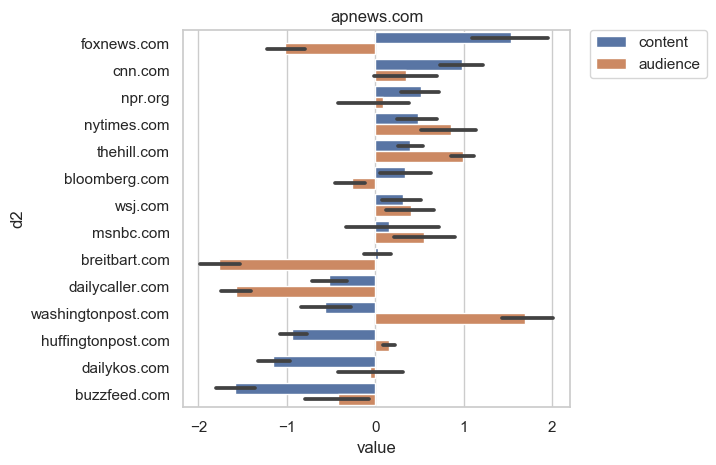
\includegraphics[width=\textwidth]{figures/ca-apnews-composite.png}
\end{figure}

\begin{figure}[H]
  \centering
  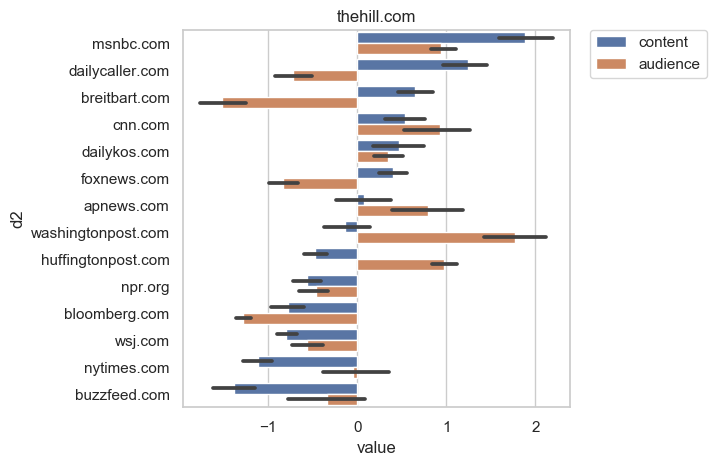
\includegraphics[width=\textwidth]{figures/ca-thehill-composite.png}
\end{figure}

\subsection{AP}

Focusing on AP first -- for AP, then, the two largest content / audience mismatches are with Fox and WaPo. AP headlines sound like Fox headlines, but the audience overlap is low; whereas, audience overlap is high with WaPo, but headline similarity is low. At first blush, then, this might suggest that AP is serving as a bridge that exposes WaPo readers to Fox-like content -- the headlines are similar to Fox, but the readership overlaps with AP. But, of course, AP is also anomalous, here, in the sense that it's in large part a wire service -- AP pushes out content through the \texttt{apnews.com} domain, but AP stories also get syndicated by other outlets. So, when AP "sounds like" Fox -- is that because AP is producing content that's similar to content produced in-house by Fox, or is it that Fox is literally running AP headlines -- in which case, the similarity getting picked up by the classifiers would be a function of AP (literally) sounding like itself?

Of course, even if Fox is syndicating AP, doesn't make it a less "real" part of Fox's content fingerprint, in the sense that the AP content is still getting distributed under the imprint of the Fox brand and getting pushed out to Fox viewers. (And there's also the Fox editorial fingerprint -- Fox surely doesn't publish all AP stories, and the selection of which ones to publish is highly substantive.) But, if the AP/Fox content similarity is primarily a function of syndication, this would somewhat change interpretation of which outlet is serving as a "bridge" -- if AP is similar to native Fox content, then could think of AP as conduit that moves Fox $\rightarrow$ WaPo, NYT, etc. But, if Fox is syndicating AP, then it would be Fox that's acting as the bridge, exposing AP content to an audience that overlaps highly with The Daily Caller and Breitbart.

The answer turns out to be interestingly mixed. To get a visual sense of the overlap -- looping back to the UMAP projection for all 15 outlets, here's just Fox:

\begin{figure}[H]
  \centering
  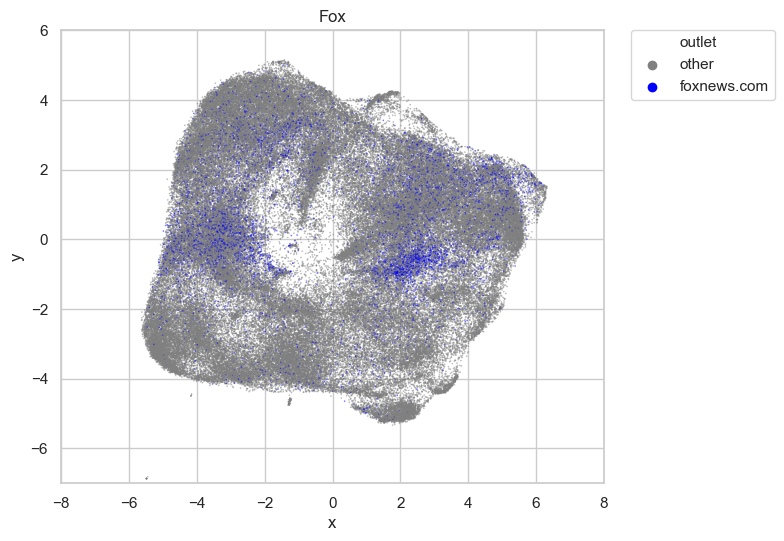
\includegraphics[height=0.4\textheight]{figures/fox-umap.png}
\end{figure}

And, here's Fox and AP, where we can see that the entire cluster of Fox headlines around \texttt{(-3, 0)} sits right on top of the main AP cluster:

\begin{figure}[H]
  \centering
  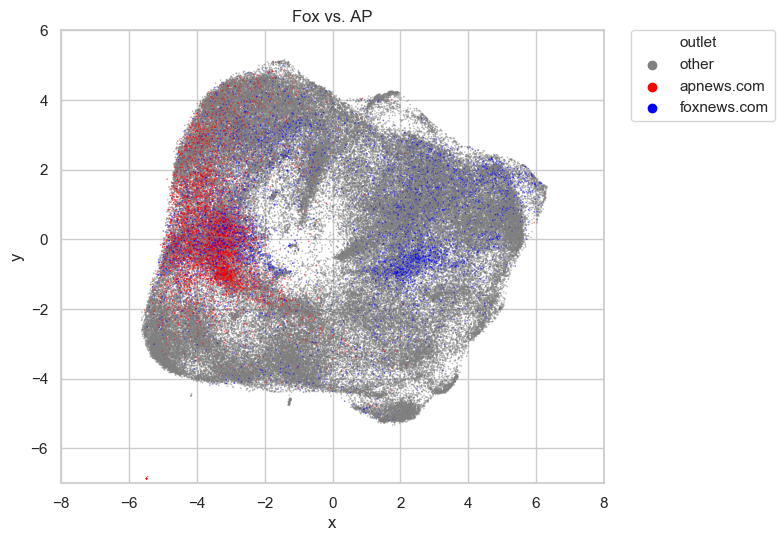
\includegraphics[height=0.4\textheight]{figures/fox-ap-umap.png}
\end{figure}

What are these headlines? To get a sense of what this overlap between AP and Fox looks like, we can use an approach similar to the technique that we used before when measuring the "diameter" of the embedding families for each outlet -- sample a large number of random pairs of headlines from AP and Fox, take the cosine distances between each pair, and then skim off the closest pairs -- headlines from Fox and AP that get mapped to very similar coordinates in the high-dimensional space. From a sample of 1 million random headlines from each outlet, here are the 20 closest Fox/AP pairs:

\begin{lstlisting}[basicstyle=\tiny\hlfont]
    AP: trump targeting irs rule on churches
    Fox: trump targeting irs rule on churches

    AP: oregon boy # found in car trunk critically injured
    Fox: indiana father charged with neglect in sons drownings

    AP: egypt gunmen attack christians killing at least #
    Fox: egypt church bombing kills at least #

    AP: dad who dragged teen daughter through school avoids prison
    Fox: man reunited with baby he saved with cpr on side of highway

    AP: iran detains ex prosecutor convicted in # torture case
    Fox: pakistani army says indian fire kills # soldiers in kashmir

    AP: iran s revolutionary guard says hit syria for tehran attacks
    Fox: egypt s islamic state affiliate claims deadly sinai attack

    AP: honduras president says open to review of disputed vote
    Fox: saudi arabia says corruption probe detainees will face trial

    AP: parents baby girl attacked by raccoon inside apartment
    Fox: mom investigating soldier son s death uncovers new evidence

    AP: # officers killed in palestinian attack
    Fox: # men believed migrants killed in greece

    AP: man jumps from car saves elderly woman from oncoming train
    Fox: dirt bike gang brutally beats driver on california highway

    AP: uk police arrest #nd man in london subway attack case
    Fox: turkish pop star journalists on trial over failed coup

    AP: # dead # injured in kentucky school shooting suspect held
    Fox: # on thunderbirds jet in ohio accident taken to hospital

    AP: minnesota sheriff # injured when school van semi collide
    Fox: colorado walmart shooting leaves # dead # injured

    AP: germany confirms that # germans killed in egypt stabbing
    Fox: china reports # alleged assailants killed in far northwest

    AP: arkansas inmate attempting to halt nov # execution
    Fox: minnesota firefighters rescue saint bernard stuck on roof

    AP: german police brace for rival protests after man killed
    Fox: ukrainian rebels say commander killed in car bombing

    AP: couple who prayed for healing plead guilty in baby s death
    Fox: # including boy dead in murder suicide amid custody battle

    AP: officer takes dying woman to beach to fulfill her last wish
    Fox: man reunited with baby he saved with cpr on side of highway

    AP: uneasy calm after # die in india riots over guru verdict
    Fox: nepali climbers say outcrop near top of everest is intact

    AP: thousands stranded as floods submerge southern indian state
    Fox: magnitude # earthquake slams south central mexico
\end{lstlisting}

All of which, we can see, have a distinctly AP flavor to them, though the content appears to focus on particular areas. Namely -- foreign affairs ("German police," "Ukranian rebels"), crime and terrorism ("Walmart shooting," "deadly Sinai attack"), and US news that's anchored by references to particular states ("Arkansas inmate," "Minnesota sheriff," "Oregon boy.") The closest pair, though, is an exact duplicate -- which, indeed is an example of an AP story that's getting syndicated by Fox. Here, on \texttt{foxnews.com}, with the byline pointing back to AP:

\href{https://www.foxnews.com/us/trump-targeting-irs-rule-on-churches}{https://www.foxnews.com/us/trump-targeting-irs-rule-on-churches}

And here on \texttt{apnews.com}:

\href{https://apnews.com/02692b5d6d684e529287396df1017877}{https://apnews.com/02692b5d6d684e529287396df1017877}

But, just spot-checking a few other headlines, there are also some from Fox that are getting produced in-house by Fox. For example, "Man reunited with baby he saved with CPR on side of highway" was written by Alexandria Hein for Fox's health section:

\href{https://www.foxnews.com/health/man-reunited-with-baby-he-saved-with-cpr-on-side-of-highway}{https://www.foxnews.com/health/man-reunited-with-baby-he-saved-with-cpr-on-side-of-highway}

What's the overall ratio here? From the set of Fox headlines that sound like AP -- how many are literally from AP? Ideally, if we had a complete set of headlines from each outlet, we could just check for exact duplicates. But, unfortunately, this isn't a reliable way to measure this, because we're working with data that passed through two layers of sampling -- first, headlines that get shared on Twitter, and second, headlines that make it into the 10\% Decahose sample. This means that there could be URLs to \texttt{foxnews.com} pages that are syndicating content from AP, but for which we don't have the corresponding "native" version of the AP article from \texttt{apnews.com}. There could be headlines from foxnews.com in the corpus, in other words, that originate from AP but don't also show up in our sample from \texttt{apnews.com}.

To get a more reliable approxiation of this, we explicitly checked this on a subset of Fox articles that look similar to AP to the model. We took the mean embedding vector for all AP articles and then queried the 500 foxnews.com headlines that are closest to the AP mean. Then, for each of these articles, we scraped the `dc.source` meta tag value from the original pages on foxnews.com, which indicates the origin of the article -- `Associated Press` for AP, `Fox News` for Fox. Out of the 500 pages, 467 had populated `dc.source` tags; and of these, 320 (69\%) were from AP, and 118 (25\%) were natively generated by Fox.

So, the truth is somewhat mixed. On the one hand, Fox is syndicating a significant number of AP stories -- all of which get pushed out to the Fox audience, and, in a kind of tautological sense, become a constitutive part of Fox's content footprint. And, alongside this, Fox also generates a non-trivial number of articles in-house, (mostly under the auspices of the "World" desk) that sound very similar to the AP headlines that are getting syndicated. In a sense, then, rather than thinking of AP as a conduit that moves right-leaning content from Fox into left-leaning WaPo feeds, it might be more accurate to interpret the flow as moving in the opposite direction -- Fox's AP-heavy content profil runs very strongly against the grain of its underlying audience structure. Fox, rather, is pushing AP-esque content into Daily Caller and Breitbart feeds. This becomes clearer when looking at Fox's full set of content / audience weights:

\begin{figure}[H]
  \centering
  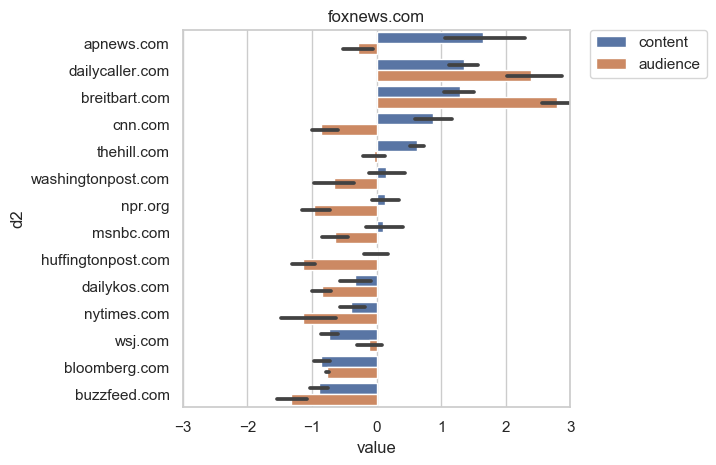
\includegraphics[width=\textwidth]{figures/ca-foxnews-composite.png}
\end{figure}

Where, clearly, the content-level similarity with AP is a very significant outlier -- Fox is \textit{closest} to AP, at the level of language, even while the audience similarity is extraordinarily concentrated in The Daily Caller and Breitbart. In this sense, then, Fox is acting as a very significant bridge between left-leaning and right-leaning audiences. By pushing out AP content -- both via literal syndication, and via original reporting that closely matches AP content / style -- Fox is pushing content into Daily Caller and Breitbart feeds that otherwise would appear primarily in WaPo, Hill, NYT, and MSNBC feeds, where AP has high audience correlation. To return to the diagrammatic view -- Fox's presence in the (-3,0) region of the embedding, overlapping with AP, represents possibly the single largest content/audience mismatch in this set of 15 outlets.

Stepping back -- what can we say about the \textit{effect} of this mismatch? When Fox pushes out this content, one interpretation is that this might act as a moderating influence, diluting feeds that are otherwise filled with highly polarized content with headlines that are relatively mainstream. But, looking at the actual content of these headlines -- the type of content from AP that Fox chooses to run with -- it's also paints a somewhat dim view of what the "common ground" between ideologically separated outlets might look like -- here, stories about foreign political unrest, domestic crime reporting, natural disasters, often anchored to specific locations. (Which, even with US states, perhaps have a rhetorical effect of making the stories seem distant, remote, removed -- only a minority of readers are in Missouri or Arkansas, let alone Germany or Saudi Arabia.) A map of violence, misfortune, wrongdoing.

\subsection{The Hill}

Beyond the AP, which is something of an outlier due to the content syndication -- the most misaligned outlet is The Hill, which has a very strange mix of content and audience similarities, and seems to be the closest thing in this set of 15 outlets to a legitimately bipartisan (or maybe cross-partisan) news source. On the one hand, high content and audience similarity with (left-leaning) MSNBC:

\begin{figure}[H]
  \centering
  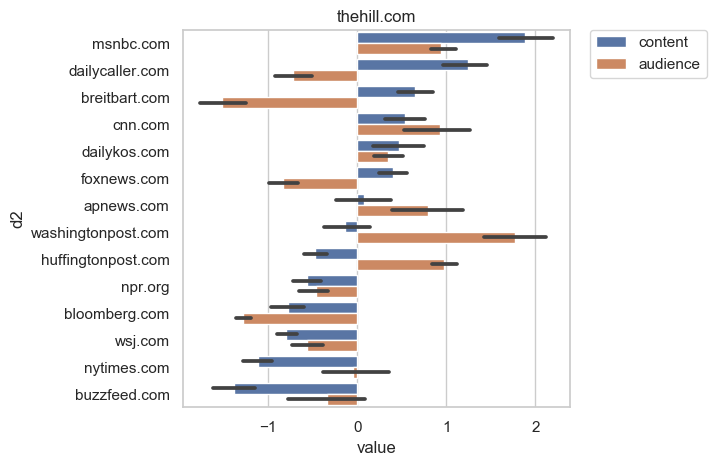
\includegraphics[width=\textwidth]{figures/ca-thehill-composite.png}
\end{figure}

But, after that, things break down -- high audience overlap with other left-leaning outlets like WaPo, HuffPo, and CNN, but relatively low content similarities with these outlets; and, higher content similarities with the (far) right-leaning Daily Caller and Breitbart. What does this overlap with the far-right blogs look like? Like before, we randomly sample 1M headlines from The Hill and Daily Caller, then find the 20 pairs with the smallest cosine distances -- a sample of the most nearby pairs of embeddings across the two outlets. For The Hill and Daily Caller:

\begin{lstlisting}[basicstyle=\tiny\hlfont]
    The Hill: dem candidate for va governor is fighting for ms #
    Daily Caller: dem donor network wants reparations on agenda by #

    The Hill: dems kick off unity commission
    Daily Caller: house dems want comey tapes

    The Hill: dem senator throws cold water on impeachment talk
    Daily Caller: dem rep slams party leadership or lack thereof

    The Hill: dems push leaders to talk less about russia
    Daily Caller: dem reads trump tweets during sessions hearing

    The Hill: dems up # points in party affiliation
    Daily Caller: dem candidates racking in record breaking donations

    The Hill: gop senator puts hold on trump energy nominee
    Daily Caller: gop reps lash out at mnuchin after meeting

    The Hill: scaramucci out as wh communications director
    Daily Caller: acosta i brought heat to wh press briefing

    The Hill: dem backed candidate wins wisconsin supreme court race
    Daily Caller: moderate dems fear lack of support from national party

    The Hill: dem calls for trump impeachment on house floor
    Daily Caller: dem candidate compares trump victory to terror attacks

    The Hill: dems prepare for fight over trump s cia pick
    Daily Caller: ny dems to protest against confederate street names

    The Hill: no surprise dem memo was nt released
    Daily Caller: dem mayor vetoes $ # min wage bill

    The Hill: tapper on michelle wolf backlash do trump supporters really want to talk about decency
    Daily Caller: ryan on trump s govt shutdown tweet i understand the president s frustration

    The Hill: dem rep demands answers on niger attack
    Daily Caller: top dem on # strategy it s being worked on

    The Hill: sanders supporters cancel clinton protest
    Daily Caller: mccain sides with media with over trump

    The Hill: senate intel dem rips twitter over deeply disappointing briefing
    Daily Caller: senate dems targeting rep price are getting richer #x faster

    The Hill: dems step up efforts to avoid california primary shutouts
    Daily Caller: dems floats public option as solution to obamacare woes

    The Hill: watch cnn anchor s disbelief that clinton aides destroyed phones with hammer
    Daily Caller: gen hertling shoots down cnn s jim sciutto having been in the military

    The Hill: alabama rep i m still backing moore because he ll vote right in the senate
    Daily Caller: morgan freeman i m holding out hope that trump will be a good president

    The Hill: trump will not approve release of dem counter to nunes memo
    Daily Caller: rnc ad campaign targets vulnerable dems over gorsuch obstruction

    The Hill: sanders to campaign in iowa with former aide
    Daily Caller: mccain sides with media with over trump
\end{lstlisting}

And, for The Hill and Breitbart:

\begin{lstlisting}[basicstyle=\tiny\hlfont]
    The Hill: nazareth mayor cancels christmas celebration over trump s jerusalem decision
    Breitbart: public broadcaster admits to increasing booing sounds during trump davos speech

    The Hill: bush era nato ambassador do we need any more evidence that trump is unfit for office
    Breitbart: cher dems must win to stop gestapo tactics of ice and impeach trump

    The Hill: house dems raised record $ # million in march
    Breitbart: dem staffers boo trump at unity baseball game

    The Hill: pot state dems want federal regulation of marijuana
    Breitbart: dems say guerrilla tactics for gun control coming

    The Hill: meghan mccain to cpac head why is nt there a modicum of respect for my family
    Breitbart: kirsten gillibrand if dems win midterms first thing we should do is abolish ice

    The Hill: dem mega donor steyer runs ads calling on hoyer to support impeaching trump
    Breitbart: dem rep introduces bill to block trump from using federal funds to pay for border wall

    The Hill: graham rips trump over anti muslim videos the antidote to terrorism is not racism
    Breitbart: cher dems must win to stop gestapo tactics of ice and impeach trump

    The Hill: dem memo does nt change anything proves intel abuse occurred
    Breitbart: dems willing to be flexible on funding for trump s wall

    The Hill: al sharpton trump on course to win in # because dems are too tame to deal with him
    Breitbart: kirsten gillibrand if dems win midterms first thing we should do is abolish ice

    The Hill: gop lawmaker rips mueller if he were more biased we d have to give him credentials for mainstream media
    Breitbart: trump slams fbi for double standard regarding dnc manafort i wo nt be involved i may change my mind

    The Hill: expect trump s state of the union to celebrate america and provide a roadmap to the future
    Breitbart: progressives despise trump so much they ve begun to dislike the country that elected him

    The Hill: seattle seahawks player trump is an idiot for saying protesting nfl players should nt be in the country
    Breitbart: maajid nawaz i m suing the splc for defamation for putting me on anti muslim extremist list

    The Hill: secret service stops man who tried to meet ivanka trump armed with throwing knives
    Breitbart: american wrestler in mexico infuriates fans with pro trump rants in the ring

    The Hill: gay us olympians continue feud with vice president eat your heart out pence
    Breitbart: obamacare mandate repeal is the most important civil rights victory in years

    The Hill: pittsburgh mayor fires back at trump my city will follow paris agreement
    Breitbart: celebrities to join women s march la on anniversary of trump inauguration

    The Hill: billy bush hits trump over access hollywood tape denials stop playing around with people s lives
    Breitbart: alabama accuser deletes anti moore postings from facebook rants about removing trump from office

    The Hill: keith olbermann i am retiring from political commentary
    Breitbart: toby keith i wo nt apologize for playing trump inauguration

    The Hill: liberal group launches database to track corporations response to tax law
    Breitbart: administration wants tax bill to pass with or without repeal of obamacare mandate

    The Hill: mattis tillerson warned trump of security concerns in israel embassy move
    Breitbart: mcconnell insider says majority leader would back garland for fbi director

    The Hill: cnn s stelter blasts trump hannity relationship let s just underscore how weird this is
    Breitbart: cnn s stelter questions trump s mental fitness is he suffering from some kind of illness
\end{lstlisting}

Where, clearly, the overlap is largely driven by a particular \textit{style} of political reporting -- a kind of professional, inside-the-beltway view on politics; politics covered as a sport, a game that plays out across a stream of interactions, quarrels, gambits, moves, calculations, confrontations. Specifically, the model is picking up on the use of a very distinctive set of abbreviations used by all three outlets -- namely \texttt{dems}, \texttt{gop}, \texttt{rep}. Likewise for MSNBC:

\begin{lstlisting}[basicstyle=\tiny\hlfont]
    The Hill: trump has abdicated his responsibility as president
    MSNBC: trump has the worst lawyers of any president

    The Hill: dems wonder can gop even pass a budget
    MSNBC: dems need more than anti trump message

    The Hill: senate dem sees looming constitutional crisis
    MSNBC: female dems plan more political engagement

    The Hill: dems will cave if republicans go
    MSNBC: dem leadership is old and creaky

    The Hill: dems fundraising off of trump comments attacking lewis
    MSNBC: dem senator vows to expose medicaid cuts in gop plan

    The Hill: trump doubles down on merck attack
    MSNBC: trump backs down repeatedly

    The Hill: cohen tape is powerful exculpatory evidence
    MSNBC: cohen wiretapping was unjustified

    The Hill: dems will oppose short term spending bill
    MSNBC: dems plan filibuster to block gorsuch

    The Hill: senate dem to intel chief answer my surveillance question publicly
    MSNBC: dem candidate for ny ag open to prosecute trump aides if pardoned

    The Hill: intel committee dems to trump read torture report
    MSNBC: dems hold lead going into # can gop rebound

    The Hill: mueller agrees to some limits on trump interview
    MSNBC: kushner downplays meeting with russians

    The Hill: nyt issues correction to giffords editorial
    MSNBC: dems shut out of immigration meeting

    The Hill: dems put squeeze on ryan over chaplain controversy
    MSNBC: dem congresswoman offers path forward for party

    The Hill: dems flip seat in florida state special election
    MSNBC: dems see record early voting numbers in texas primary

    The Hill: dem candidate for va governor is fighting for ms #
    MSNBC: dem rep has full confidence in fbi director comey

    The Hill: gop should remove nunes as intel chairman
    MSNBC: trump must give intel unambiguous praise

    The Hill: dems announce unity commission members
    MSNBC: media clamp down at white house press briefings

    The Hill: midterms pose dilemma for mueller
    MSNBC: new proposed legislation would protect mueller

    The Hill: dems step up attacks on gop obamacare bill
    MSNBC: dems demand nunes evidence by friday

    The Hill: dems hit trump on national coming out day
    MSNBC: dems have emergency plan if trump fires mueller
\end{lstlisting}

Though, it's also not just this lexicon of political slang words that's driving these pairings. To put this into relief -- if we use the same procedure to identify headlines that mark the overlap of The Daily Caller and Breitbart, a very different portrait of these outlets emerges:

\begin{lstlisting}[basicstyle=\tiny\hlfont]
    DC: illegal alien arrested for allegedly sexually assaulting # young girls
    BB: illegal alien charged for alleged rape and murder of sanctuary city woman

    DC: cnn s chris cuomo tries to justify antifa s violent tactics are they equally wrong
    BB: cnn s jim sciutto spreads fake news about trump revoking brennan s security clearance

    DC: illegal alien arrested for allegedly sexually assaulting # young girls
    BB: previously deported illegal alien accused of raping # year old thousands of times

    DC: ice arrests two criminal illegal immigrants after nj county declines detainers
    BB: ice operations collar nearly # criminal illegal immigrants in two states

    DC: german leaders propose bringing refugees to visit concentration camps to combat anti semitism
    BB: truckers claim french switching off uk funded equipment intended to stop illegal calais migrants

    DC: migration expert more than # million muslims would support terrorists
    BB: fatah marks anniversary by celebrating terrorists who murdered israelis

    DC: brennan implies trump could start a war to divert negative media attention from himself
    BB: david lynch responds directly to trump you could be a great president if you reverse course

    DC: baltimore sun media critic david zurawik calls for nbc to investigate joy reid
    BB: hannity predicts book deal msnbc contributorship and maddow colbert maher bookings for comey

    DC: california college tuition going up but not for illegal alien students
    BB: children cry on tape after border apprehension illegal alien mother convicted

    DC: milo s dangerous incinerates the left confounds the gop and trolls everyone in between
    BB: john kirby it bothers me that trump s afghanistan speech is being given at fort myer

    DC: cartel thugs who murdered ice agent get life in prison
    BB: media ignore americans killed by illegal alien dreamers

    DC: dem response to trump s immigration plan is wildly out of touch with american voters
    BB: dem strategist james devine launches hashtag huntrepublicancongressmen after steve scalise shooting

    DC: jennifer rubin melts down asks if people against amnesty are raised by wolves
    BB: maxine waters leftist bullies and their media enablers want to disarm us

    DC: dem candidate compares trump victory to terror attacks
    BB: biden warns dems do nt walk out of kavanaugh hearings

    DC: dhs spokesman we re allowed to arrest deport illegal alien crime victims at courthouses
    BB: nationwide manhunt for three illegal aliens accused of kidnapping raping teen sisters

    DC: exclusive tucker report carter page contacted trump campaign after fisa warrant was granted
    BB: former wasserman schultz it staffer allegedly uploaded terabits of information to dropbox

    DC: muslim leaders march throughout europe in protest of islamic terrorism
    BB: east london murder suspect used welfare benefits to join islamic state

    DC: jeff sessions announces zero tolerance policy following surge in illegal border crossings
    BB: left s narrative trump administration pro rape for scrapping obama campus sex policies

    DC: mitch mcconnell gave trump a present after passing tax reform it s too perfect
    BB: nancy pelosi called the tax cut worst bill in history here s why that s ridiculous

    DC: obama state department let clinton and huma make off with boxes of muslim engagement docs
    BB: schumer fake news women turn to planned parenthood for mammograms maternity care
\end{lstlisting}

Focused heavily on (Mexican, Central American) "illegal aliens" and (Islamic) terrorism; often invoked in racially charged and xenophobic contexts. Which, looking back at the overlap between these outlets and The Hill, is (almost) entirely absent. So, it seems as if The Hill overlaps with a particular aspect of these right-leaning outlets -- what might be thought of as the "sport of politics," for lack of a better phrase -- politics as a kind of drama, a competitive arena; but stripped, in large part, of the charged ideological substance that marks the headlines at the overlap of Breitbart and The Daily Caller.

In different ways, then, can think of AP and The Hill as marking scraps of common ground in the media ecosystem -- we can look to these sites of mismatch as indicators for the types of coverage that attract attention from outlets that occupy disparate regions of the audience graph. From AP -- foreign political instability and crime; from The Hill -- politics as sport.

\subsection{Taxonomies of (mis)match}

Beyond these two most dramatic misalignments, there are a number of other intersting patterns that can be seen with other outlets that at times seem to suggest different "taxonomies" for the content-audience fit, the range of diffrent ways that an outlet can occupy these graphs. For example, Huffington Post has extremely low audience correlations with Fox, Daily Caller and Breitbart, even though the content distances are right around average; suggesting, perhaps, a very strong ideological aversion between the audiences of HuffPo and these outlets, even though the headline distance is par for the course.

\begin{figure}[H]
  \centering
  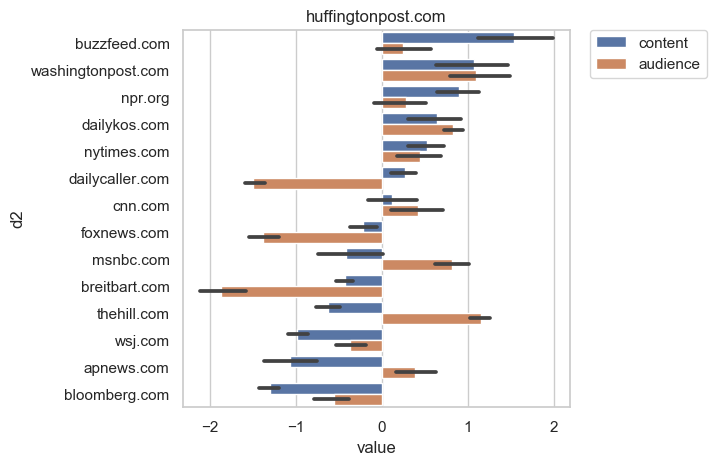
\includegraphics[width=\textwidth]{figures/ca-huffingtonpost-composite.png}
\end{figure}

The Washington Post, meanwhile, is notable for having very high audience correlations with a number of other left-leaning outlets -- NYT, MSNBC, The Hill -- even though the headline similarities are relatively low; suggesting, perhaps, that WaPo represents a voice that is both consistently different from other left-leaning outlets but also consistently interesting to audiences of other left-leaning outlets. (Perhaps a function of WaPo's somewhat unique role as both a national political outlet and D.C. local paper?)

\begin{figure}[H]
  \centering
  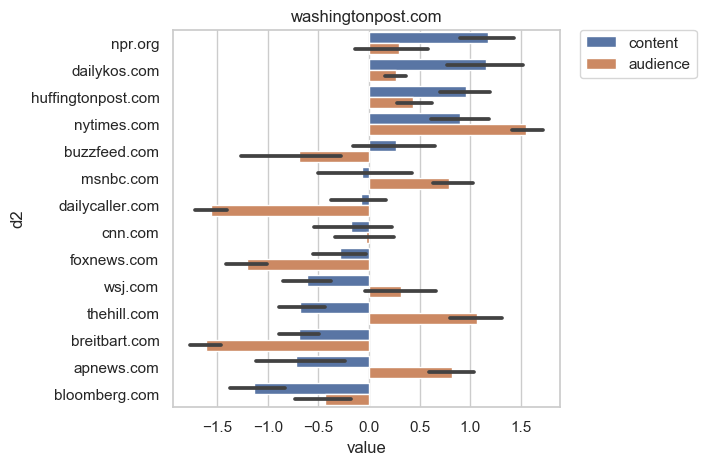
\includegraphics[width=\textwidth]{figures/ca-washingtonpost-composite.png}
\end{figure}

Last but not least, the three most right-leaning outlets -- Fox, Breitbart, and The Daily Caller -- all have very similar profiles -- strong audience correlations with each other and low audience overlap with everyone else; but a much more continuous distribution over headline similarities, with AP and The Hill registering unexpectedly high similarities with Fox and Daily Caller respectively, which run strongly against the grain of the audience-level similarities.

\begin{figure}[H]
  \centering
  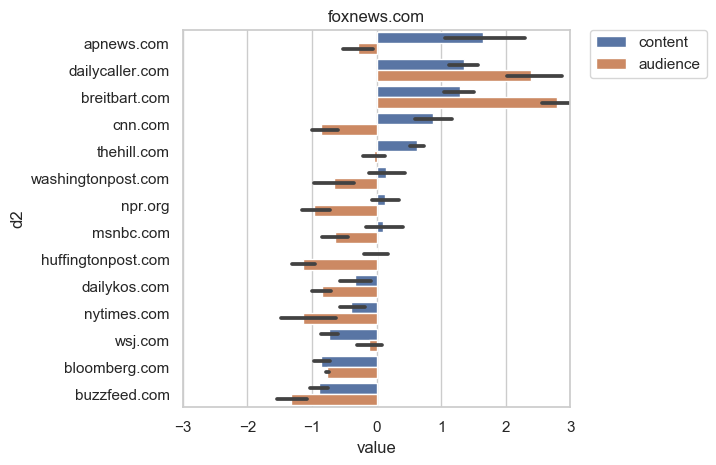
\includegraphics[width=\textwidth]{figures/ca-foxnews-composite.png}
\end{figure}

\begin{figure}[H]
  \centering
  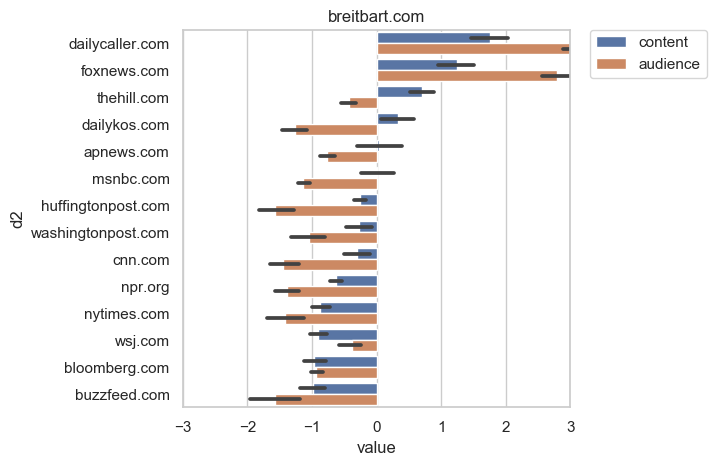
\includegraphics[width=\textwidth]{figures/ca-breitbart-composite.png}
\end{figure}

\begin{figure}[H]
  \centering
  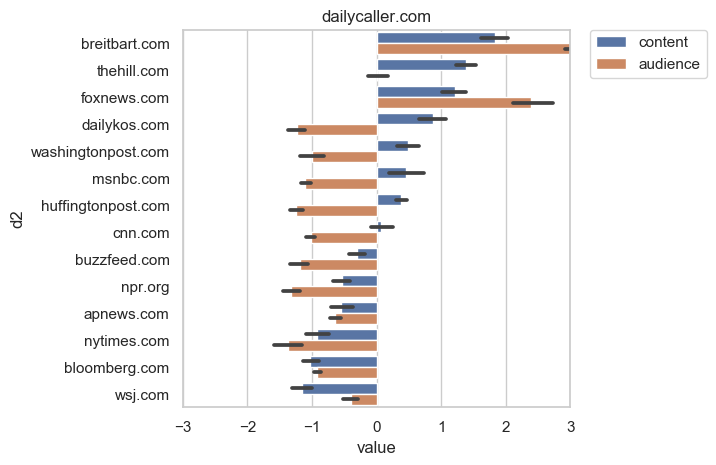
\includegraphics[width=\textwidth]{figures/ca-dailycaller-composite.png}
\end{figure}

\section{Headlines as a historical process}

By measuring the \textit{distinguishability} of headlines, then, we are able to construct a precise representation of the relative similarities and differences among media outlets. Then, we compared these content-level similarities to similarities at the level of audience, which makes it possible to identify sites of misalignment between these graphs, places where outlets "speak" in ways that are more or less similar than we would expect, given the composition of their audiences. Fox distributes a large slice of AP content that doesn't fit into Fox's overall linguistic niche; The Hill occupies an unusual middle-ground in the landscape of political reporting, producing headlines that the classifiers mistake for both the center-left MSNBC and the far-right Breitbart and Daily Caller. The underlying audience graph, in other words, provides an initial point of comparison for the headline-level similarities -- a way to throw them into relief, systematically identify edges in the content graph that are stronger or weaker than we might expect.

An immediate question arises from this, though -- how "new" or "old" are the relationships that emerge in these two graphs? So far, though, we've been treating the headlines as a completely synchronic slice of data -- we're rolling up 625 days of data into a single unit. In a sense, though, this represents a fairly radical deformation of the underlying data -- more than almost any other type of textual object, headlines are fundamentally situated at specific moments in time, intended to be read in the context of very tight temporal windows -- anywhere from a few weeks down to a few house. If we imagine a kind of uber-text of the news, the full mass of content produced by all news outlets -- then individual headlines form a kind of emergent syntagmatic chain -- a progression, a linear movement forward through a sequence of events, stories, opinions.

Intead of rolling up the data into a single unit -- what if we add back in the timestamps on the original links, and study the headline space as a diachronic system, unfolding over 625 days? This opens the door to an intriguing set of questions. Instead of just modeling the overall structure of the content/audience relations among outlets -- could we track the evolution or "drift" of these relations over time? How stable are they? Do they change at all? And if they do -- how? Are there pairs (or groups) of outlets that have become significantly more or less similar over time, at the level of the headline? Would it be possible to identify high-level patterns of convergence or divergence in the news media -- subsets of outlets that have drifted, over time, into higher or lower levels of "shared attention"? We can imagine a kind of "plate tectonics" of the media landscape, playing out at the level of textual distance -- a set of slow (or not so slow?) shifts, as news organizations shift into new regions of content / style, and into new configurations relative to each other.

How to model this? If the synchronic analysis produced a fully-connected graph over the set of 15 outlets, a weighted adjacency matrix -- how to unroll this over time? How to "unroll" each edge in the graph over the 625 days in the data window? One approach would be to simply take the outputs from models trained on synchronic data and reintroduce timestamps post-hoc during analysis. For example, we could take test-set predictions from the LSTM -- which is trained simultaneously on all data from across the full window of data -- and look at changes in the structure of the predictions according to the timestamps on the underlying tweets.

This could be useful as a way to start reasoning about the actual contnt of changes over time -- for example, the types of headlines that are most typical of an outlet at one point in time relative to another. But, as a means of \textit{measuring} changes over time and identifying the most significant shifts, there are some potential risks with this. First, very simply -- as we saw earlier, a number of outlets have undergone large changes in the raw quantity of content that they have produced over the time period in question. For example, counting the number of unique articles that circulate on Twitter each day, HuffPo produced less than 50\% as much content in the summer of 2018 than in the spring of 2017. Because of this, a model trained on the full dataset would see significantly more examples of 2017 headlines from HuffPo than 2018 headlines, which would likely make it less accurate on the 2018 data. Which, then, if we take classification accuracy as a proxy for distance, might give the appearance that HuffPo is getting more similar to some other outlet(s) -- classification accuracy is falling -- when in fact the score is just proxying the underlying change in volume.

We could guard against this by, for example, splitting the data into deciles and then downsampling each outlet to an equal size in each decile. But, even with this, there could be risks associated with trying to capture fine-grained changes over historical time from a model trained without any knowledge of temporal differences. To take an example from a similar domain -- Ted Underwood notes that topic models, when used to produce vectors that represent the topic distributions of texts, can produce misleading "banding" effects at the edges of the historical range of the corpus.\cite{underwood2018warp} For example, here, the Y-axis represents the angular distance between topic vectors for books published immediately before and after the year on the X-axis -- an attempt to model the "speed" at which the corpus is changing, taking each year as a pivot point.

\begin{figure}[H]
  \centering
  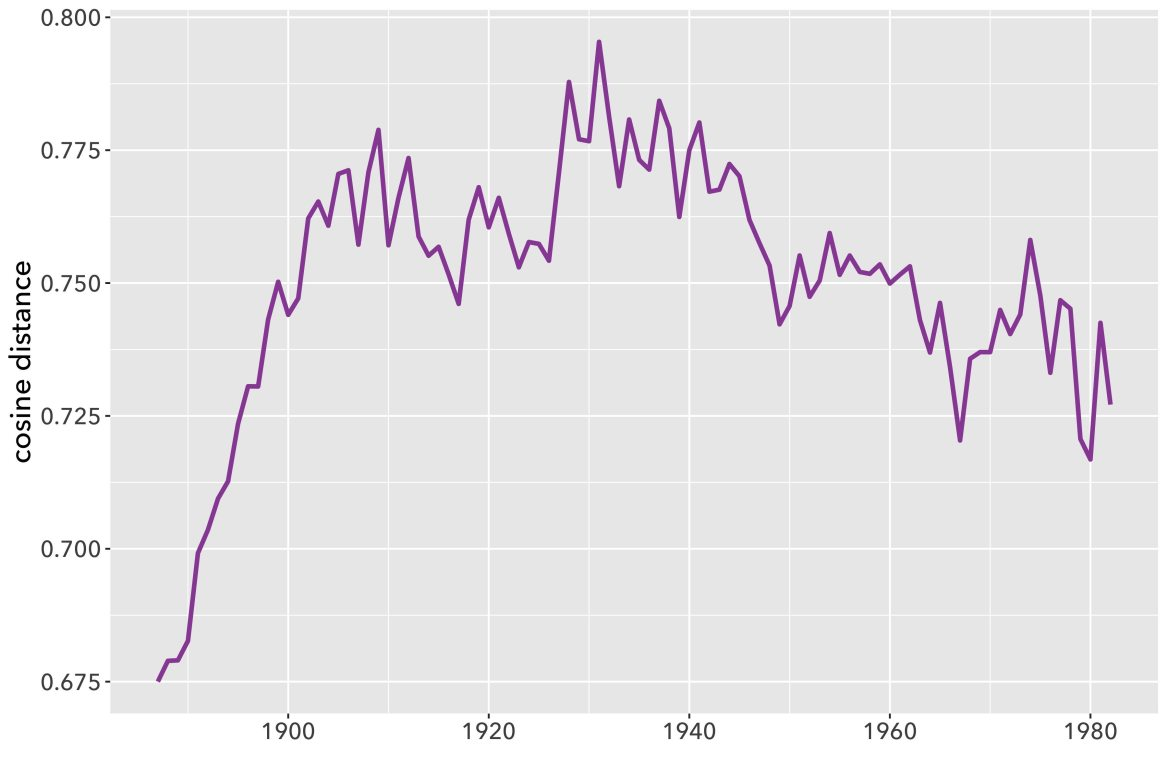
\includegraphics[width=0.5\textwidth]{figures/tm-banding-1.jpg}
  \caption{"Do topic models warp time?" Underwood.}
\end{figure}

From this plot, it appears that the corpus changes very quickly at first, and then the rate levels off and starts to fall. But, Underwood notes, if you re-fit the model on data from different time spans that partially overlap -- for example, if you add or remove 25 years of data to the start of the corpus -- it turns out that this arc-shaped pattern crops up again and again, in a way that contradicts the results from the other slices of data. Clearly, this is some kind of modeling artifact -- all of these can't be true:

\begin{figure}[H]
  \centering
  \includegraphics[width=0.5\textwidth]{figures/tm-banding-2.jpg}
  \caption{"Do topic models warp time?" Underwood.}
\end{figure}

Underwood doesn't pin down a cause for this. But, in a broad sense, it seems that the model is somehow optimizing around the "middle" of the data at the expense of the edges -- what looks like a meaningful historical change is probably just an artifact of how the model is solving the optimization problem.

To my knowledge this kind of thing hasn't been systematically explored with neural classifiers, and it's possible that neural models would be less susceptible to this sort of thing. But, out of an abundance of caution -- how can we get an initial view on this that almost certainly avoids this type of problem? An easy route, which we take here, is just to train a very large battery of completely independent models on different historical slices of the data. The downside to this, of course, is that this become much more computationally expensive than just training a single model on all of the data at once -- ideally, we would do this with the strong neural models, but this would take many hundreds or thousands of hours of GPU time. But, like before with the A-vs-B comparisons between individual pairs of outlets, if we forgo the neural models and fall back to the non-neural baselines, these training runs can be easily parallelized on cheap commodity hardware, which makes it feasible to train a very large number of independent comparisons.

Which particular model and similarity metric should we use for these comparisons? The linear SVC is particularly attractive in that (a) it's the strongest non-neural baseline, just 3\% off the LSTM, and (b) it fits very quickly, making it feasible to train hundreds of thousands or even millions of individual models. But -- how "trustworthy" are the similarity scores produced by the SVC? Conveniently, building on the large grid of similarity scores explored in section \ref{section:hl-graph}, we can quantify this by simply taking the mean squared error between the accuracy scores produced by the SVC and the mean value for all metrics, and then compare this score across all metrics. Sorting from lowest to highest error, we find that the SVC pairwise accuracy is close to the top of the list -- the similarity measured by the SVC is generally very close to the average score derived from all metrics. This gives confidence that we can use the SVC as an accurate (and, importantly, highly efficient) representation of similarity.

So, using the SVC classification accuracy as a canonical signal for similarity -- how to measure historical changes in proximity across the 15 outlets? If we had an indefinite amount of data, we could simply split the data into a large number of non-overlapping buckets, and then fit models on data from each bucket independently. But, in this case, we're limited by the size of the dataset from the lowest-volume outlet, which defines the size of the data samples we pull from each outlet, since these always need to be held constant to ensure that the similarity scores are comparable. (Here, again, this is MSNBC, with 18k headlines in total.) If we split this over, say, 100 buckets, this falls to just ~180 headlines per bucket, which is very small. We could just split over fewer buckets -- say, 10 -- which would make it possible to train on 1800 headlines per outlet per bucket. This is better, but, 10 buckets also gives a much more blocky, discretized view of the historical interval, which, depending on where the bin boundaries happen to fall, might somewhat obscure interesting trends.

To get a somewhat continuous approach, while still maintaining a decent quantity of data in each time slice, we take this approach -- first, split the data into 100 equally-sized bins, and then slide a 10-bin rolling window across these bins. So, the first window would include bins 1-10; the second, bins 2-11; the third, bins 3-12; and so on. This gives a total of 91 partially-overlapping windows across the data, each individually covering 10\% of the total temporal interval.

As initial smoke test -- considering all outlets, has the overall "differentiability" across the 15 outlets changed over time? Here, we fit all-versus-all multiclass models on 100 random size-balanced samples across each of the 91 windows. In each window, we randomly sample 18k headlines from each outlet, split this sample of 270k headlines into standard 80/20 train-test splits, fit a SVC classifier on the training data, and then evaluate accuracy on the test set. And then repeat this sampling process 100 times for each window, giving a total of 9,100 all-vs-all accuracy scores:

\begin{figure}[H]
  \centering
  \includegraphics[width=\textwidth]{figures/ts-ava.png}
\end{figure}

Where, again, high classification accuracy can be interpreted as low similarity (the outlets are easier to tell apart) and low accuracy can be interpreted as high similarity (outlets are more difficult to distinguish).

So, there seems to be some trend, though the error bands are fairly large here -- an early high-water mark of differentiability in the winter and spring of 2017 (immediately following Trump's inauguration), and then a fairly consistent falloff over the course of the next 18 months, and then a sudden spike in the summer and fall of 2018. But, this is a somewhat constrained view, since it's hard to make sense of what might be driving the change. When the accuracy suddenly spikes at the end of the window -- is that because all of the outlets are simultaneously becoming more differentiated from each other? Or, are these changes driven just by a smaller subset of outlets that become more distinguishable to the model, but which has the effect of pushing up the overall accuracy score?

To get a clearer view of this, broken out by individual outlets -- we can do the same thing again, but this time training "one-vs-all" models for each outlet in each window. So, for example, for the New York Times in window 10 -- we first sample 18k random headlines from all outlets, like before; but then, holding out the 18k headlines from the New York Times -- the "foregrounded" outlet -- we randomly sample 18k headlines from across all of the other 14 outlets. This gives two sets of 18k headlines -- the "foreground" set, for the New York Times, and the "background" set, evenly sampled from everything else. We can then fit a regular binary model on these two splits, which will give a measurement for the degree to which that individual outlet is distinguishable with respect to all others at that particular moment in time. Like before, this is repeated on 100 random samples for each outlet in each window, giving a total of 136,500 accuracy scores, which can then be grouped by outlet. Here, sorted by the slope of a linear fit, sorted from most increasing to most decreasing:

\begin{figure}[H]
  \centering
  \includegraphics[height=\textheight]{figures/ts-ova.png}
\end{figure}

Now, the shape of things starts to come into closer focus -- the sudden rise in accuracy at the end that was visible in the all-vs-all accuracies is clearly driven almost entirely by BuzzFeed, which becomes rapidly and dramatically more distinctive at the very end of the data window, the accuracy jumping by almost 10\% in just a couple of months. Fox, meanwhile, has the strongest overall linear trend, becoming consistently more differentiated over the 18-month window, maybe with something of a phase shift at the end of 2017. Meanwhile, at the other end of the spectrum, four outlets show consistent falloffs in differentiability -- The Hill, The Daily Kos, Huffington Post, and CNN.

But -- falloffs relative to what? These trends make it possible to pick out the outlets that are driving the overall trend, but it's not clear how the individual changes relate to each other. For example, when The Hill falls from 72\% to 68\% accuracy, it's becoming more "confusable" with some combination of other outlets. But, which outlets? With everything else rolled into a single "other" category, it's hard to make sense of why this is happening. What we need, again, is to model the complete matrix of relationships among all outlets -- but here, the relationships represent the degree to which every outlet has become more or less similar over time, not just the overall similarity.

To get at this -- in the same way that we could train a battery of individual A-vs-B models to get pairwise similarity scores when modeling the structure of the (synchronic) content graph, we can do the same thing again, but here broken out across each of the 91 temporal windows. For each of the 104 unique pairs over the 15 outlets, and in each of 91 windows, we sample 18k headlines from outlet A, 18k for outlet B, and then fit a binary model; and then repeat this 100 times, to get a distribution over 100 sampled classification accuracies for each pair of outlets in each window -- a total of 955,500 model fits.

With this, we can break out a historical similarity trend for each individual pair. Again, sorting by the slope of a standard linear fit, here are the 10 pairs with the strongest increases in accuracy, pairs that have moved away from each other most significantly over the last 2 years:

\begin{figure}[H]
  \centering
  \includegraphics[height=\textheight]{figures/ts-ab-rising.png}
\end{figure}

Most of these pairs include either BuzzFeed or Fox, paired with a number of different outlets, suggesting that these two outlets are becoming consistently more differentiated from a fairly wide range of other sources -- they drifting off into increasingly isolated, individually distinctive linguistic spaces. Meanwhile, in the other direction -- here are the 10 pairs with the strongest linear decreases in classification accuracy -- outlets that \textit{converged} most significantly over time:

\begin{figure}[H]
  \centering
  \includegraphics[height=\textheight]{figures/ts-ab-falling.png}
  \caption{}
  \label{fig:ts-ab-falling}
\end{figure}

Here, again, we can spot a handful of outlets that crop up in a number of different pairs -- Huffington Post (in particular, present in each of the top three), The Daily Kos, and The Hill.

Moving beyond just the 10 strongest trends in each direction -- from the full set of 105 pairwise relationships, we can assemble the fully connected graph for all 15 outlets. Here, we treat the slopes of the regression fits as signed edge weights between the outlets. The width of the edge represents the absolute magnitude of the slope -- the degree to which the relationship between the pair has changed over time -- and the color represents the direction -- blue for negative slopes, where outlets have become more similar over time (lower classification accuracies), and red for positive slopes, where outlets have become more dissimilar (higher classification accuracies).

\begin{figure}[H]
  \centering
  \includegraphics[height=0.5\textheight]{figures/ts-ab-radial.png}
\end{figure}

From this, a number of clear trends start to fall out. First, there seems to be a core group of outlets that have undergone a significant convergence over the last two years -- Huffington Post, The Hill, Daily Kos, CNN. (All left-of-center, it's worth noting.) And, to a lesser extent, AP, The Washington Post, The New York Times and NPR have all become more confusable with some combination of these four, though in a somewhat more patchy and inconsistent way (Daily Kos, in particular, has become more confusable with WaPo, NYT, and NPR). Meanwhile, BuzzFeed and Fox have moved in the opposite direction -- they have become more differentiated from \textit{almost every single other outlet}. (And, notably, Fox has diverged significantly from WSJ, second only to the movement away from BuzzFeed.) Though, of all outlets, Huffington Post has maybe the most mixed and extreme pattern of movements -- it moves dramatically away from BuzzFeed (the single largest decrease in similarity) and converges strongly with CNN, Daily Kos, and The Hill.

This makes it easier to reason about the full structure of all 105 pairwise accuracy changes, but, it still isn't a complete picture. One disadvantage to the classification metric, in this context, is that it's \textit{undirected}. We know, for example, that CNN and HuffPo have become more "confusable" with each other, but this could happen in a few different ways -- it could be that CNN headlines have migrated in the direction HuffPo; or, HuffPo could have shifted towards CNN; or both towards each other; or some mix of all of these. Or, with Fox, which becomes easier for the model to distinguish from almost every other outlet -- it could be that every other outlet is independently moving away from Fox, or that just Fox is moving away from everything else.

Modeling this explicitly is tricky, and in a sense requires some kind of "anchoring" of the data outside of the pure notion of textual distance that we've been using in this study.\footnote{It's possible that we could get at this by looking at relative positions in the embedding spaces in the neural models -- for example, if outlets A and B become more confusable over time, we could try to figure out which outlet started out farther away from the combined ending position of the two. Which had to "travel" farther, essentially?} Provisionally, though -- how to block in a very rough sketch of this? It turns out that a number of things start to become clear just from just looking at changes undergone by some of the individual outlets involved in the strongest pairwise shifts. For example, with something like BuzzFeed -- what exactly is driving the sudden, huge spike in accuracy that kicks off in July of 2018? Which headlines are responsible for this?

In theory, we could try to get at this by looking the decision functions learned by the SVMs -- for example, look at headlines that were confused by the model in different periods, or look at what kinds of headlines get placed very far from the decision boundary. But, really, this kind of question about the actual content of the headlines calls out for the types of distributed representations learned by the neural models. The SVMs give a controlled, highly-sampled snapshot of the \textit{degree} to which outlets have reconfigured over time. As triangulation of this -- could we explore the \textit{substance} of these changes by treating them as movements in the vector space induced by the neural models?

To ensure that all outlets are evenly represented in all time periods, we split the data into 10 deciles, and then sample an even number of headlines for each \texttt{(domain, decile)} pair. Then, we re-train the original all-vs-all models on this time-balanced corpus, which produces a set of embeddings for each outlet in each temporal decile of the corpus.

With this in hand, to get a sense of how these outlets have shifted over time, we can query for individual headlines that are \textit{most characteristic of the overall geometric movements in the embedding space}. For example, to find headlines that, for the model, "typify" the movement of BuzzFeed between the beginning and end of the data, we can take \texttt{mean(BuzzFeed 2018) - mean(BuzzFeed 2017)}, and then find the individual BuzzFeed headlines with the smallest angular distance from this difference vector -- headlines that mark BuzzFeed in 2018, specifically in comparison to BuzzFeed in 2017. Here are the top 20:

\begin{lstlisting}[basicstyle=\tiny\hlfont]
    answer these five questions and we ll tell you which shrek character you are in bed
    build your high school life and we ll reveal which character you are from finding nemo
    take a trip to the beach and we ll tell you which summer bop you should listen to
    pick a movie from each year and we ll tell you which comedy show you belong on
    check off all the classic disney movies you ve seen and we ll guess how old you are
    tell us your perfect night in and we ll tell you which literature lady you are
    create a breakup playlist and we ll tell you which iconic movie character you were in a past life
    tell us your favorite female tv character and we ll tell you what your greatest strength is
    plan a movie night and we ll tell you which character from the incredibles you re most like
    decorate your apartment with uo decor and we ll reveal which celebrity will live with you
    plan your dream first date and we ll tell you how old your soulmate is right now
    make a break up playlist and we ll tell you which marvel superhero you re most compatible with
    pick nine random things and we ll tell you which sex and the city girl you are
    create your perfect fall day and we ll tell you what book to read next
    choose your meals for the day and we ll tell you which parks and rec character you are
    choose your fave cartoon grandparents and we ll give you an activity to do with your grandparents
    make a breakup playlist and we ll tell you which marvel superhero you re most compatible with
    eat at taco bell and we ll tell you which avenger would be your best friend
    plan your perfect hogwarts feast and we ll tell you which house table to sit at
    tell us your harry potter preferences and we ll give you a european city to visit this summer
\end{lstlisting}

This suggests, then, that the rise in accuracy for BuzzFeed in the summer of 2018 is driven by a sudden explosion of this "quiz" genre, of the form "[Do a quiz], and [we'll tell you something about yourself]." Going in the other direction, though, gives a clearer sense of the overall shift. Here's \texttt{mean(BuzzFeed 2017) - mean(BuzzFeed 2018)}, headlines that mark the beginning of the corpus as compared to the end:

\begin{lstlisting}[basicstyle=\tiny\hlfont]
    as trump takes office birth control startups see demand spike
    trump hotel contractor drops $ # million lawsuit
    taiwanese court delivers landmark ruling in favour of marriage equality
    trump administration punts again on obamacare subsidy lawsuit
    congressmen seek to lift propaganda ban
    trump picks patriot act lawyer for top state department job
    us and cuba to open diplomatic relations in historic agreement
    north carolina officials seek to stop special elections
    obama warns inequality could derail climate change efforts
    police fired gas at protesters outside trump s rally
    mike pence on confederate statues i m someone who believes in more monuments not less
    libyan dissident wins right to sue ex foreign secretary jack straw over rendition
    clinton iowa volunteers train when to push backers to omalley to block bernie
    guardian ditches move to kushner building after newsroom revolt
    alex jones suffers defeat in custody hearing
    bannon ally leaves white house as mcmaster consolidates power
    devos first # days marred by rollbacks missteps and blunders
    britain heads to the polls
    texas sues over feds withholding of overseas execution drugs
    uk general election polling day and count
\end{lstlisting}

Which, in essence, is simply \textit{politics}. So, BuzzFeed's ratio of political-coverage-to-clickbait has gone down; in terms of its overall content profile, BuzzFeed is moving away from political coverage, towards quizzes.

What about Huffington Post, the outlet that BuzzFeed has diverged with most significantly? Moving in chronological order this time -- here's \texttt{mean(HuffPo 2017) - mean(HuffPo 2018)}, headlines that are distinctive of HuffPo at the beginning of the window:

\begin{lstlisting}[basicstyle=\tiny\hlfont]
    connecting food and your mood
    a tale of two globalizations
    a true omnichannel experience reaps the biggest rewards
    the rise of deaftalent
    yes you can get bbq from a drive thru
    what s your dietary footprint
    the problem with tickling
    how s your grammarly mine s great
    the genius trick for oatmeal that ll make your mornings easier
    how many people are vegetarian
    the future of work is collective
    a beginner s guide to digital advertising
    do women really need a yearly pelvic exam
    tired of mid century modern try these cozy couches instead
    how to create thought leading ideas
    your gut feeling fear or intuition
    make your goals stick
    how to make vegan parmesan cheese and make your dreams come true
    how dieting makes you gain weight
    how do you know if your therapist is helping you
\end{lstlisting}

Which, though very distinct from BuzzFeed's quizzes, might fall under the same broad rubric of "entertainment" or "lifestyle" content -- here, maybe with a particular focus on diet and food. Meanwhile, headlines that are distinctive of HuffPo at the end of the window are dominated by politics:

\begin{lstlisting}[basicstyle=\tiny\hlfont]
    trump honors fallen soldiers on memorial day with self congratulatory tweet
    omarosa claims trump has mental decline that could not be denied
    tennessee man accused of burning black man alive was known white supremacist
    ambien maker denounces roseanne barr for blaming racist tweet on insomnia drug
    editorial cartoonist critical of trump fired from pittsburgh newspaper
    man yelling about trump opens fire in president s florida golf club
    susan collins receives # coat hangers ahead of kavanaugh vote
    tsa apologizes to ny giants player for spilling mom s ashes during bag search
    man who refused to hand over immigrant info to ice do nt collaborate with fascists
    federal prosecutor put on leave for targeting maxine waters with hateful facebook post
    karl rove likens trump to stalin tells him to tone down anti press rants
    tennessee pastor resigns after admitting sexual incident was abuse of power
    florida dem candidate for governor relying on vocal trump supporter
    country star gretchen wilson arrested after altercation on american airlines flight
    it s time to decriminalize immigration say top texas dems
    gop rep duncan hunter wife indicted by grand jury in san diego
    mollie tibbetts relative slams racist fear mongering and white house hyperbole
    conservatives and liberals alike find gun ban at nra s pence event hypocritical
    late night writer vows to take red hats back from trump supporters
    georgia cop suspended after liking racist kkk facebook posts
\end{lstlisting}

So, Huffington Post has undergone a kind of exact inversion of BuzzFeed's evolution. To return to the question of \textit{directionality} -- here, seems as if BuzzFeed and Huffington Post are both independently moving away from each other. BuzzFeed is shifting away from politics and towards clickbait; HuffPo is shifting away from clickbait and towards politics.

What about Daily Kos, which, as we saw in figure \ref{fig:ts-ab-falling}, has become significantly harder to tell apart from a large number of other outlets -- NPR, WaPo, NYT, CNN? (Daily Kos, in fact, is involved in 6 of the 10 largest increases in similarity.) To the extent that these outlets are all share a broad ideological orientation, it's perhaps tempting to read this as a kind of convergence in the content and style of left-leaning political reporting over the course of the first 18 months of the Trump presidency. But, just from looking at Daily Kos, which is the clear "central" node in this set of changes, it seems as if this might actually driven by Daily Kos simply becoming less focused on politics. Here are the headlines that mark spring of 2017 for Daily Kos, which are almost completely focused on the trump administration -- some combination of "trump," "gop," and "republican" appears in almost every one:

\begin{lstlisting}[basicstyle=\tiny\hlfont]
    is trumpcare just a way for paul ryan to achieve his true dream of destroying medicare
    rep jamie raskin nails the gop s blatant healthcare hypocrisy every american should see this
    the everything terrible the trump administration has done so far omnibus week #
    republicans have a solution to finding the votes they need for their healthcare bill massive bribery
    q poll on trumpcare backing this bill could be very hazardous to your political health
    joe biden on trumpcare it s enough to make your blood boil
    by reviving the trumpcare zombie tom macarthur may have lobotomized his own career
    the photo of a regretful trump supporter is going viral on donald s own playground twitter
    promises promises donald trump s made them and trumpcare will break them
    the fight continues daily kos proudly endorses three great democrats to resist the trump agenda
    how incompetent is paul ryan the house might have to revote on zombie trumpcare
    this is not normal republican senators in the dark on trumpcare bill they ll vote on soon
    are republicans learning from their trumpcare failure of course not
    forget that confirmation nonsense trump s state dept pick will absolutely get a full senate vote
    aarp is onto mitch mcconnell s trumpcare tricks wo nt let republicans play dumb
    special committee or special prosecutor devin nunes can not be trusted to investigate trump
    trump promises tea party groups he will punish america if trumpcare fails he will let aca fail
    do nt call it trumpcare us trumpcare trumpcare trumpcare you own it pal trumpcare
    republicans are weaponizing the census to further disenfranchise non white non straight americans
    top republican looks at facts from trumpcare s cbo score and all he has to say is fake news
\end{lstlisting}

Whereas, the headlines that mark fall 2018 are strikingly light on politics:

\begin{lstlisting}[basicstyle=\tiny\hlfont]
    teachers flee success high school
    freed from death row sabrina butler smith s story
    uk identifies russians who made nerve agent attack on skripals
    selling fossils lizard origins probiotic flies
    north korea snubs united states on talks over returning war dead
    retired teacher sentenced to # # months in case brought by energy transfer partners
    for starters bernie say his name
    individuals can change world mumbai man drives beach clean ups species return
    stone age cow surgery high carbon grasses ocean churning shrimp
    investing in early childhood education means big long term gains
    opt out of high stakes testing begins this week
    bad news hodgkin s has returned
    wells fargo blames computer glitch for hundreds of customers lost homes
    purported drone footage of texas tent city for separated children released by bbc
    amazon delivery drivers report wage theft and other abuses
    criminal charges in manhattan wage theft and insurance fraud case
    november coming into focus
    it came from outer space
    but her pocketses the inside scoop on wheat robot peer pressure
    day sixteen kremlinannex #pm et
\end{lstlisting}

Again, it's important to remember that these lists aren't representative samples of the outlets from different time periods -- rather, they're the headlines that most precisely characterize the change that has occurred between the beginning and the end, or vice versa. The Daily Kos, of course, hasn't stopped covering politics; but, this suggests that it's somewhat less \textit{exclusively} focused on politics that it was in the first months of the Trump administration. Which in turn has made it more difficult for the classifiers to tell apart from a number of other more general-interest outlets.

Last but not least, what about Fox? Which, again, has shifted away from almost everything else -- WSJ, BuzzFeed, CNN, WSJ, NYT, WaPo, and even other conservative outlets like Breitbart and Daily Caller -- it appears to be drifting off into some largely unoccupied linguistic space, far from everything. Moving chronologically -- here are headlines that mark Fox in spring of 2017 relative to fall of 2018:

\begin{lstlisting}[basicstyle=\tiny\hlfont]
    haier boss looks far beyond appliances
    are government leaders turning a blind eye toward debt
    power prices in focus as heat wave hits
    china s geely to buy lotus take stake in malaysia s proton
    investment fund providing financing for health care
    peru s finance minister quits over audio recordings
    taiwan holds war games simulating chinese island attack
    india s modi discusses trade ties with turkey s erdogan
    eurozone economic sentiment at near decade highs
    biggest movies to look forward to in #
    republicans struggle to resuscitate health bill
    ancient root with modern benefits
    get the fugitives back from cuba
    many students voted twice in uk election
    fewer fret over more focus on politics
    strong winds dry forests fuel portugal fires
    severe bolivian drought hurts crops threatens capital
    bao bao ready for new life in china
    alitalia workers vote on cuts to stave off bankruptcy
    mayim bialik to register as muslim
\end{lstlisting}

Quite a bit of general political news -- often with an economic angle -- and international stories. In the other direction -- stories that mark 2018, compared to 2017:

\begin{lstlisting}[basicstyle=\tiny\hlfont]
    florida man drops meth off at sheriff s office for testing after suffering bad reaction police say
    stars rally around liberal james gunn after offensive tweets unlike reaction to trump supporting roseanne barr
    professor banned from restaurant for profanity laced rant against white children university investigating
    washington state store clerk left to die by teen robbers after suffering heart attack cops say
    nbc news president noah oppenheim killed ronan farrow s harvey weinstein expose to protect his hollywood ambitions report says
    florida school resource officer slams unruly student to ground do nt give me your sh
    new jersey cops used sex toy big blue to harass co workers played game with genitals lawsuit says
    cheryl slams nasty false liam payne breakup reports says her mom has absolutely nothing to do with any of it
    papa john schnatter allegedly refused to work with kanye west because of n word in his lyrics
    anne hathaway calls out white privilege in wake of black woman stabbed to death at bart station
    colorado police officers suspended for leaking body camera footage of denver mayor s son yelling at cop
    cnn star jim acosta rips kim kardashian s prison reform meeting with trump but lauded john legend s activism on same during obama years
    shark in shallow water reportedly spooks beachgoers on north carolina s bald head island
    a horrible day for democracy jeff flake blasts mccabe firing encourages # primary challenge to trump
    illinois death penalty would be reinstated for mass murderers cop killers under gov rauner s proposal
    ocasio cortez claims solidarity with cab drivers while campaign buys rides from uber other alternatives fec data show
    wwe legend jerry lawler s son reportedly on life support after attempting suicide in his jail cell
    until the kneeling happened fl police union official backs call to return nfl tickets over protests
    fury as feminist activist says she s confused seeing black man with pro nra and tea party bumper stickers
    chloe bennet confirms she s dating logan paul by defending the decision to fans
\end{lstlisting}

Which is a very distinctive list -- for lack of a better word, it's a sort of "tabloid" style, focusing on crime (often grisly, bizarre), misbehavior, personal misfortune, and socially charged political issues. This suggests, then, that the "departure" of Fox -- its monotonic rise in distinctiveness, the shift away from almost all other outlets -- is defined by a movement away from (relatively) centrist political and business reporting, and in the direction of something like the National Enquirer.

\begin{figure}[H]
  \centering
  \includegraphics[width=\textwidth]{figures/ts-ova-fox.png}
\end{figure}

Stepping back, and doubling back to the original idea of modeling a kind of linguistic "plate tectonics" of the media ecosystem -- this is just a start, but from these examples we can start to reason about some of the most significant changes. BuzzFeed has doubled down on clickbait, perhaps at the expense of political reporting; HuffPo has done the opposite, shifting away from clickbait and towards political reporting; and, Fox and The Daily Caller have drifted off in the direction of a sensationalized and hyper-partisan style of coverage.

\section{Shifting headlines, shifting audience?}

We've found, then, that the "content graph" and "audience graph," treated as synchronic systems, generally tend to correlate with each other -- though to varying degrees, and wit with some notable exceptions. And, from studying historical changes in classification accuracy across the full graph of outlets, we have identified pairs and cohorts of outlets that migrated into different linguistic configurations over time -- HuffPo is shifting away from BuzzFeed and towards The Hill and DailyKos; BuzzFeed is doubling down on clickbait; Fox is moving away from almost everything else, shifting away from standard political reporting and towards a more senstaionalized tabloid style. The "content graph," then, is a dynamic system -- the composite view we got in section \ref{section:hl-graph} is a kind of synchronic blending of a system that looks different, in subtle but significant ways, in fall of 2018 versus winter 2017.

But, this suggests one final step -- which, really, is a point of entry into a larger set of questions about how these content- and audience-level relationships interact over time, and how changes to one might affect the other. In section \ref{section:content-audience}, we asked -- does the (synchronic) content graph align with the (synchronic) audience graph? Mostly, it seems that it does. But -- does this also hold for the \textit{diachronic} content graph and \textit{diachronic} audience graph? That is -- as outlets become more or less different, does this correlate with parallel changes in the composition of their audiences? For example, as Fox headlines move away from Breitbart headlines, do their audiences also become less similar? Or, as HuffPo moves towards The Hill, do the audiences converge? Of course, the question of causality here is complex, and beyond the scope of this study, which is fundamentally descriptive.  (It's entirely possible, for example, that changes in audience would drive changes in content, not the other way around.) But, as a first pass on this, just at a correlational level -- do these two trends seem to be connected at all?

Methodologically, it's not hard to get a preliminary snapshot of this. In the same way we can unroll the headline graph over historical time, we can also model diachronic changes in audience similarity in the same way. Using the same set of temporal windows over the data, we simply calculate the audience correlations over each pair of outlets in each window. This gives a time-series trend for the correlation of each pair of outlets, which we can then directly compare to changes in the headline similarities.

The results are very mixed, and in many ways create more questions than they answer. In some cases, movements in content / audience appear to be very tightly correlated. For example, Bloomberg and Fox have moved in almost perfect lockstep over the last two years -- as the headlines have become less similar, the audience has also become less similar:

\begin{figure}[H]
  \centering
  \includegraphics[width=0.7\textwidth]{figures/bloomberg-fox-corr.png}
\end{figure}

But, in other cases, there appears to be a strong \textit{negative} correlation. For example, again with Fox -- headlines from Fox and Breitbart have become steadily less similar, but the audience correlation has consistently increased over this time:

\begin{figure}[H]
  \centering
  \includegraphics[width=0.7\textwidth]{figures/breitbart-fox-corr.png}
\end{figure}

These are two of the strongest relationships -- the full set of 105 pairs distribute fairly continuously between these extremes, though with more positive correlations than negative:

\begin{figure}[H]
  \centering
  \includegraphics[width=\textwidth]{figures/ts-ca-corrs.png}
\end{figure}

And, zooming in on a larger set of the strongest pairs in each direction:

\begin{figure}[H]
  \centering
  \includegraphics[height=0.6\textheight]{figures/ts-ca-pos-corrs.png}
  \caption{Pairs of outlets with the strongest positive content-audience correlations.}
\end{figure}

\begin{figure}[H]
  \centering
  \includegraphics[height=0.6\textheight]{figures/ts-ca-neg-corrs.png}
  \caption{Pairs of outlets with the strongest negative content-audience correlations.}
\end{figure}

What to make of this? It's somewhat mysterious, and in many ways, it generates more questions than it answers. With the positive correlations, if we posit that the headline similarity is driving the audience similarity, then the interpretation seems fairly straightforward -- these outlets produce content that is "fungible," in a sense? That is -- there's a market for a particular type of content, and as two outlets start to produce more of it, readers intersted in that content will tweet more links to both outlets. But, are the headlines actually leading the audience changes? Sometimes it looks like yes, but other times, the opposite. Another possible complication -- there's some possibility that changes in the audience composition could directly affect the same of headlines that we get, since the corpus emerges from reader behavior. For example, if some external pressure causes the audience composition of NYT to shift torwards a group that's intersted in, say, foreign affairs, then this new audience might then tweet more foreign affairs articles, which in turn might cause more of these headlines to make it into the Decahose sample. (At the same time, though, this would likely be buffered by the fact that the headline-level similarities just based on the set of \textit{unique} articles associated with each outlet, and ignore the "performance" of the individual articles. The question, really, is whether changes in audience would affect the long tail of less popular content that gets lifted into the decahose.) The causality, in other words, could run in either direction, and could play out at different levels; and, there could be feedback loops between content-driven and audience-driven effects.

Whatever the cause of the positive correlations, though, they would seem to do little to explain the negative correlations. As Fox and Breitbart become less similar, at the level of headlines, they become more similar at the level of audience. Why? Maybe something like -- readers have a kind of "slot" for an outlet like Fox or Breitbart, and when they produce similar content, users tweet one of the two outlets, but not both? And, as they become less similar they start to occupy different slots, and get tweeted together? But, if this is true for Fox/Breitbart -- why not for Fox/Bloomberg, CNN/NPR, etc?

It's also also possible that there could be idiosyncratic or exogenous pressures that affect these trends that have little to do with any kind of substantive interplay between content and audience. For example, if a handful of very high-profile users start tweeting a pair of outlets alongside each other, this could then diffuse out to their followers in various ways, both via literal retweets and just general imitation. Broadly -- to really understand these, we would need to dig quite a bit deeper.

\section{Problems, questions, future directions}

We started by modeling a very precise representation of the "content graph," the degree to which headlines produced by different outlets are similar and different. Then, we compared these language-level similarities to the underlying "audience graph," and found that media organizations with similar linguistic profiles also tend to have similar audiences -- though with some signficant exceptions. Then, we unrolled the headline similarities over time, and identified outlets that have "drifted" in linguistic space to focus on different topics or styles over the course of an 18-month window. And, last, we started to explore the much larger question of how these two systems -- content and audience -- interact with each other over time. Which, in turn, opens the door to a much larger set of questions about how changes in language impact the composition of the audience, and vice versa.

Along the way, we encounted a handful of uncertainties and challenges that could be addressed by future treatments of these questions. In particular:

\begin{enumerate}
\item It's clear that the classifiers are able to pick up on differencs at the level of topic and word choice -- what's being covered, which words are being used. But, it's less clear how much they are able to model what might be thought of as the \textit{stance} of the coverage -- the ideological positioning, implications, suggestions of a headline. For example, with the The Daily Caller -- a number of different models agreed that The Daily Caller sounds (comparatively) similar to the Daily Kos, about one standard deviation above the average score for all permutations of outlets:

\begin{figure}[H]
  \centering
  \includegraphics[width=\textwidth]{figures/ca-dailycaller-composite.png}
\end{figure}

Which is perhaps unintuitive, in the sense that The Daily Caller is (very) right-leaning, and The Daily Kos is (very) left-leaning; it's not entirely clear how to make sense of this, and it seems possible that a human reader might disagree, depending on the framing of the question.\footnote{Though, of course, it's also possible that this is evidence that our expectations are wrong, not the model -- that The Daily Caller and The Daily Kos are less ideologically separated that we might think. Such is the epistemological push-and-pull of this type of large-scale text analysis -- we only trust the method if the results are broadly intuitive, but the intellectual payoff often lies in the anomalies, places where the analysis surfaces something surprising.} More likely than not, the model is picking up on a high level of "shared attention" between the two -- The Daily Kos and The Daily Caller both focus mainly on political issues, which results in a highly overlapping set of topics, names, and keywords in the headlines. For example, maybe both produced a large number of headlines with the token "kavanaugh" in them, during the Supreme Court confirmation hearings.

But, it's not clear to what degree (or if) the models are able to pick up on the political stance of the two outlets, which is quite separate -- they might have a high overlap of "attention," but a very low overlap of "viewpoint." The model might say that two headlines are similar, but a human reader might recognize that the same issue is being depicted in very different way, and score the headlines as dissimilar. Which of these is "better" or "correct"? This gets back to the basic difficulties of measuring textual distance noted by Underwood -- there are different ways that headlines can be similar and dissimilar, and modeling the question in terms of \textit{distinguishability} might mix these together in a way that makes them difficult to pull back apart at an interpretive level. Though, as Underwood shows -- distinguishability might also be better than the alternatives.

Ultimately, to really evaluate this, it would be interesting to ground-truth these models at a kind of psycholinguistic level with real human readers. Returning to the thought experiment from the beginning, where we're shown a headling and asked to guess the outlet -- what if we literally did this, and then compared the human performance on, for example, the Daily Kos / Daily Caller comparison to the model's performance?

\item Second, at a more brass-tacks level -- at times this thesis switches back and forth between different model architectures in the context of a single analysis, which is less than ideal. Namely, in the analysis of how headlines have changed over time, wher we first used the SVM to model the trends, and then switch back to the neural models to understand and interpret the trends. This is just due to cost -- ideally, everything would use the stronger neural models, but this would require hundreds or thousands of hours of GPU time, which isn't feasible given current resources.
\end{enumerate}

Independent of these methodological questions about how measure and interpret textual distance -- at a conceptual level, next big step, perhaps, is to shift from descriptions of correlation to accounts of causation. This thesis describes the linguistic and social structure of the media ecosystem in a number of ways; but this type of analysis runs up against fundamental difficulties at the level of explaining \textit{why} we see what we do, at a kind of mechanistic, causal level.

Possibly, a number of questions here call out for a more experimental treatment. For example, on the question of whether and how changes in language can trigger changes in audience -- say that a news outlet that doesn't generally use any kind of shortened "slang" words started to replace "democrats" with "dems" in a series of headlines -- but left everything else unchanged. Would this cause any uptick in engagement from readers of Breitbart and The Daily Caller, which often use "dems"? Or would the content itself have to substantively change? Broadly -- how does (and doesn't) language actually exert a kind of pressure on the world, and how might we leverage this to promote a more healthy public sphere?

\bibliography{thesis}{}
\bibliographystyle{plain}

\end{document}
